\chapter{Resultados numéricos capítulo 3}

\section{kEDMD para modelos epidemiológicos}

\begin{figure}[htbp]
    \centering
    \begin{subfigure}[b]{0.45\textwidth}
        \centering
        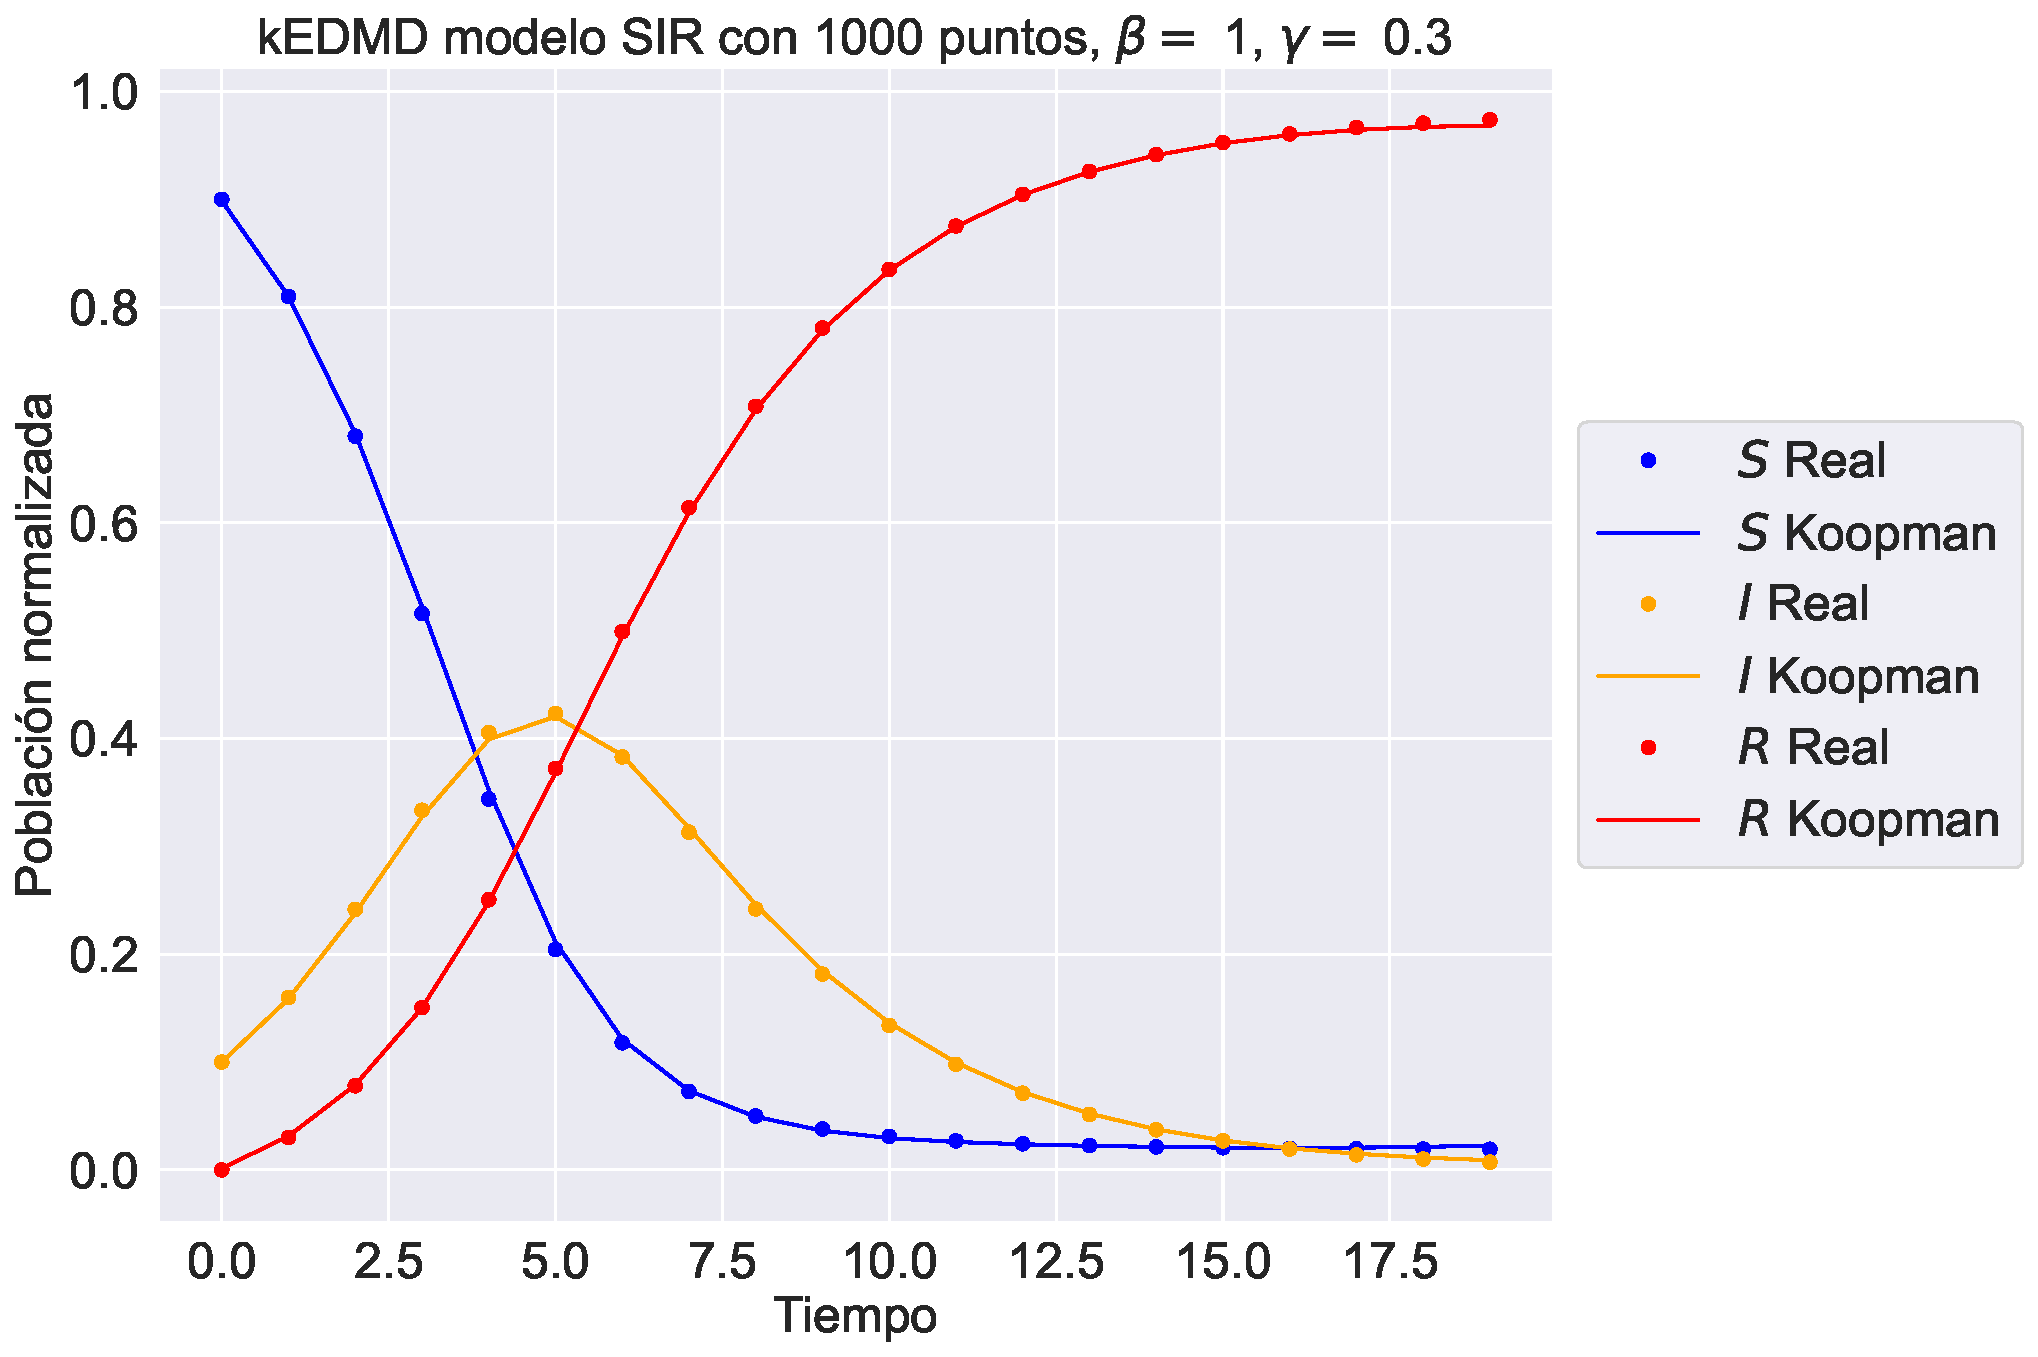
\includegraphics[width=\textwidth]{img/content/chapter3/SIR1.pdf}
        \caption{$\beta=1$, $\gamma = 0.3$}
        \label{fig:image1}
    \end{subfigure}
    \hfill
    \begin{subfigure}[b]{0.45\textwidth}
        \centering
        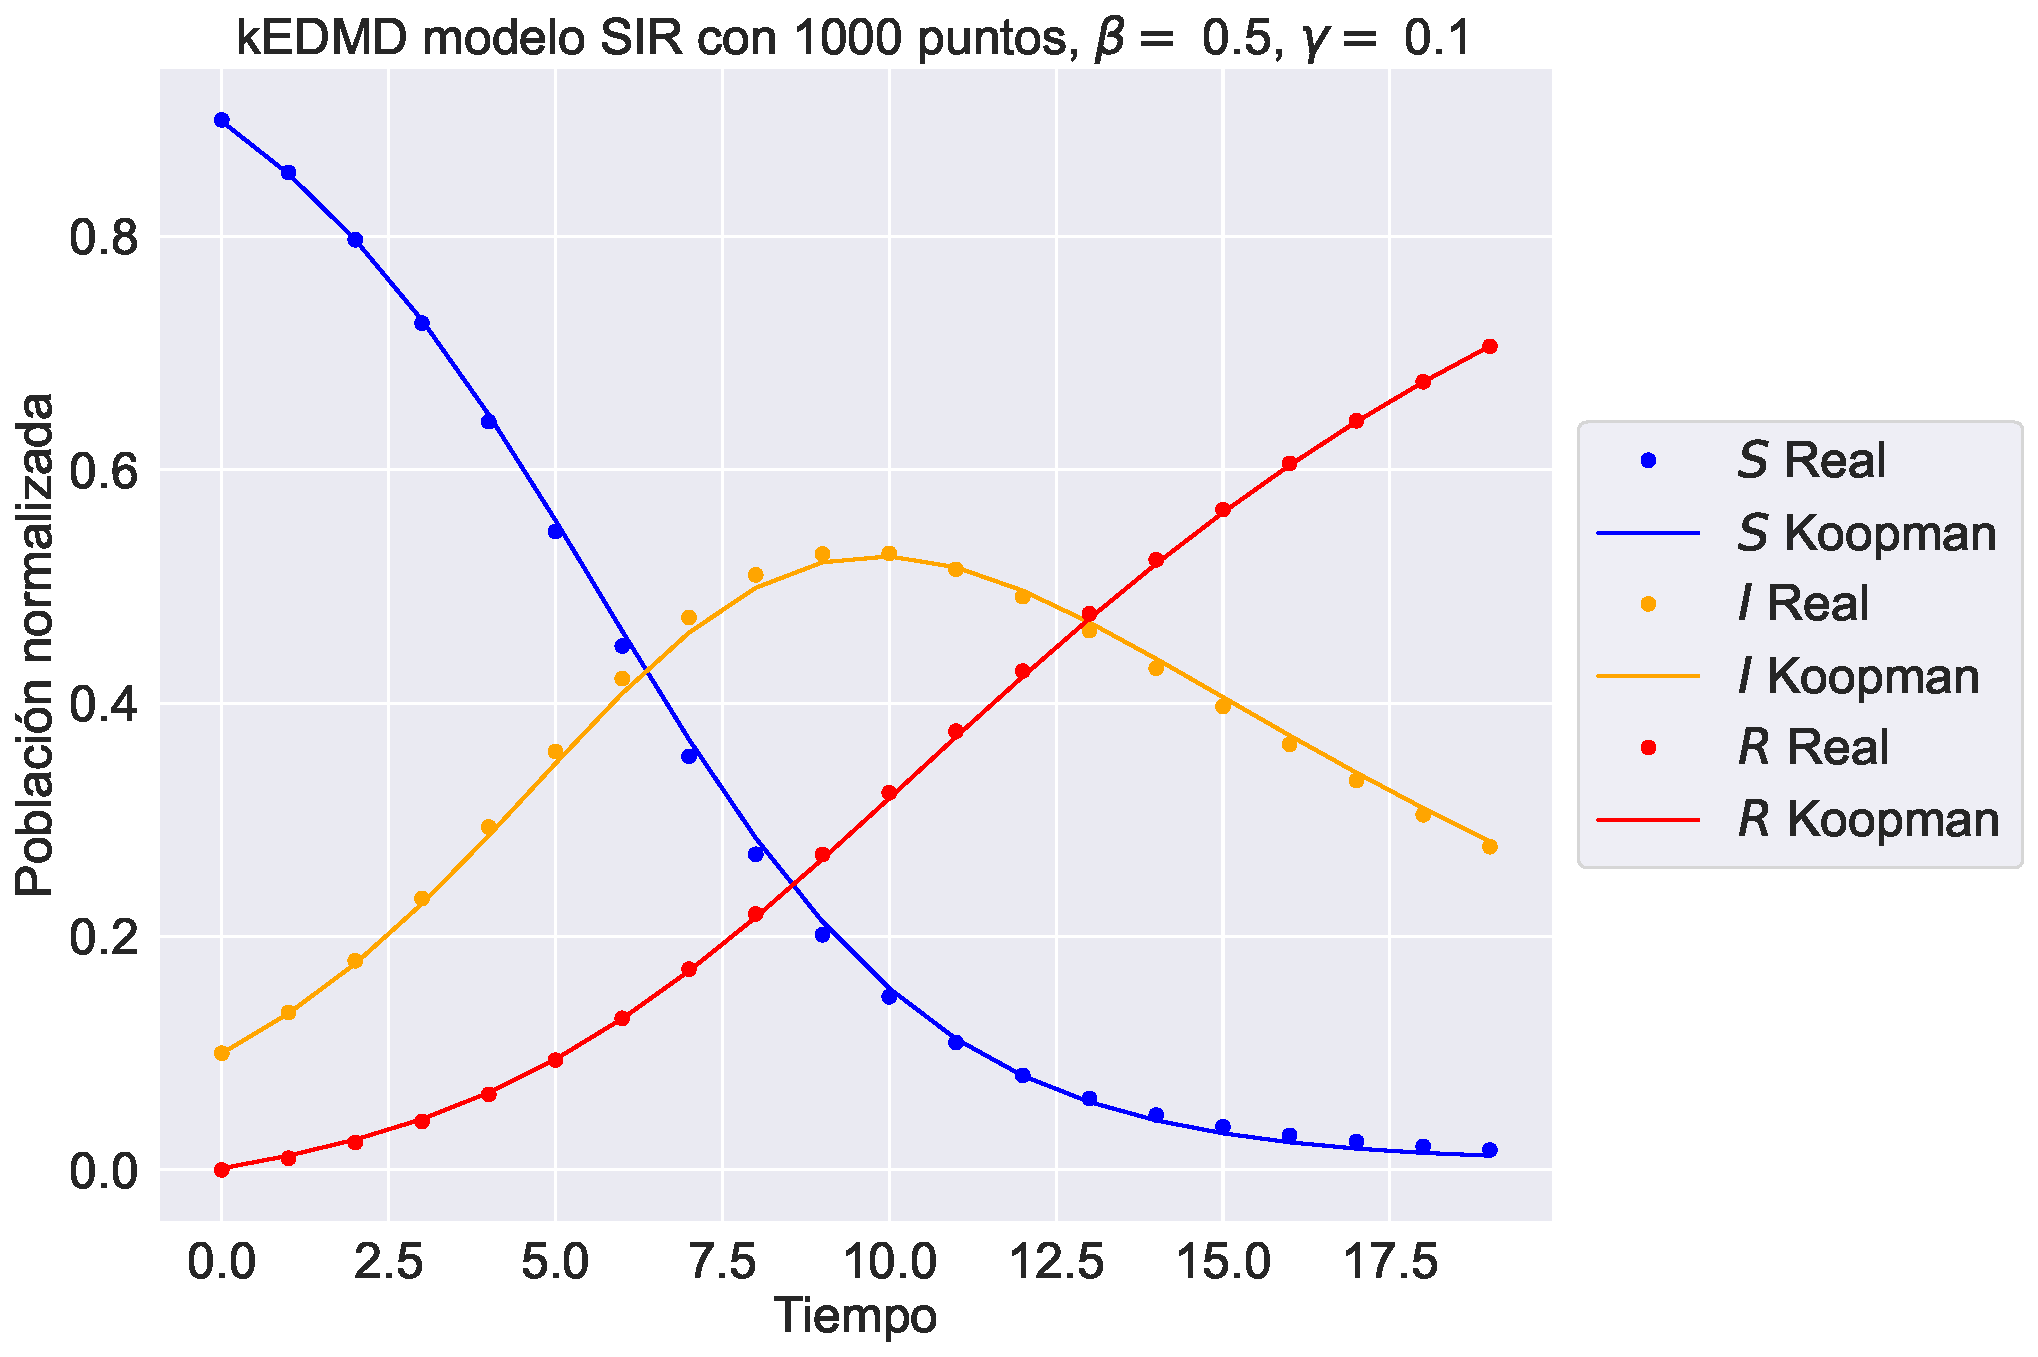
\includegraphics[width=\textwidth]{img/content/chapter3/SIR2.pdf}
        \caption{$\beta=0.5$, $\gamma = 0.1$}
        \label{fig:image2}
    \end{subfigure}
    \hfill
    \begin{subfigure}[b]{0.45\textwidth}
        \centering
        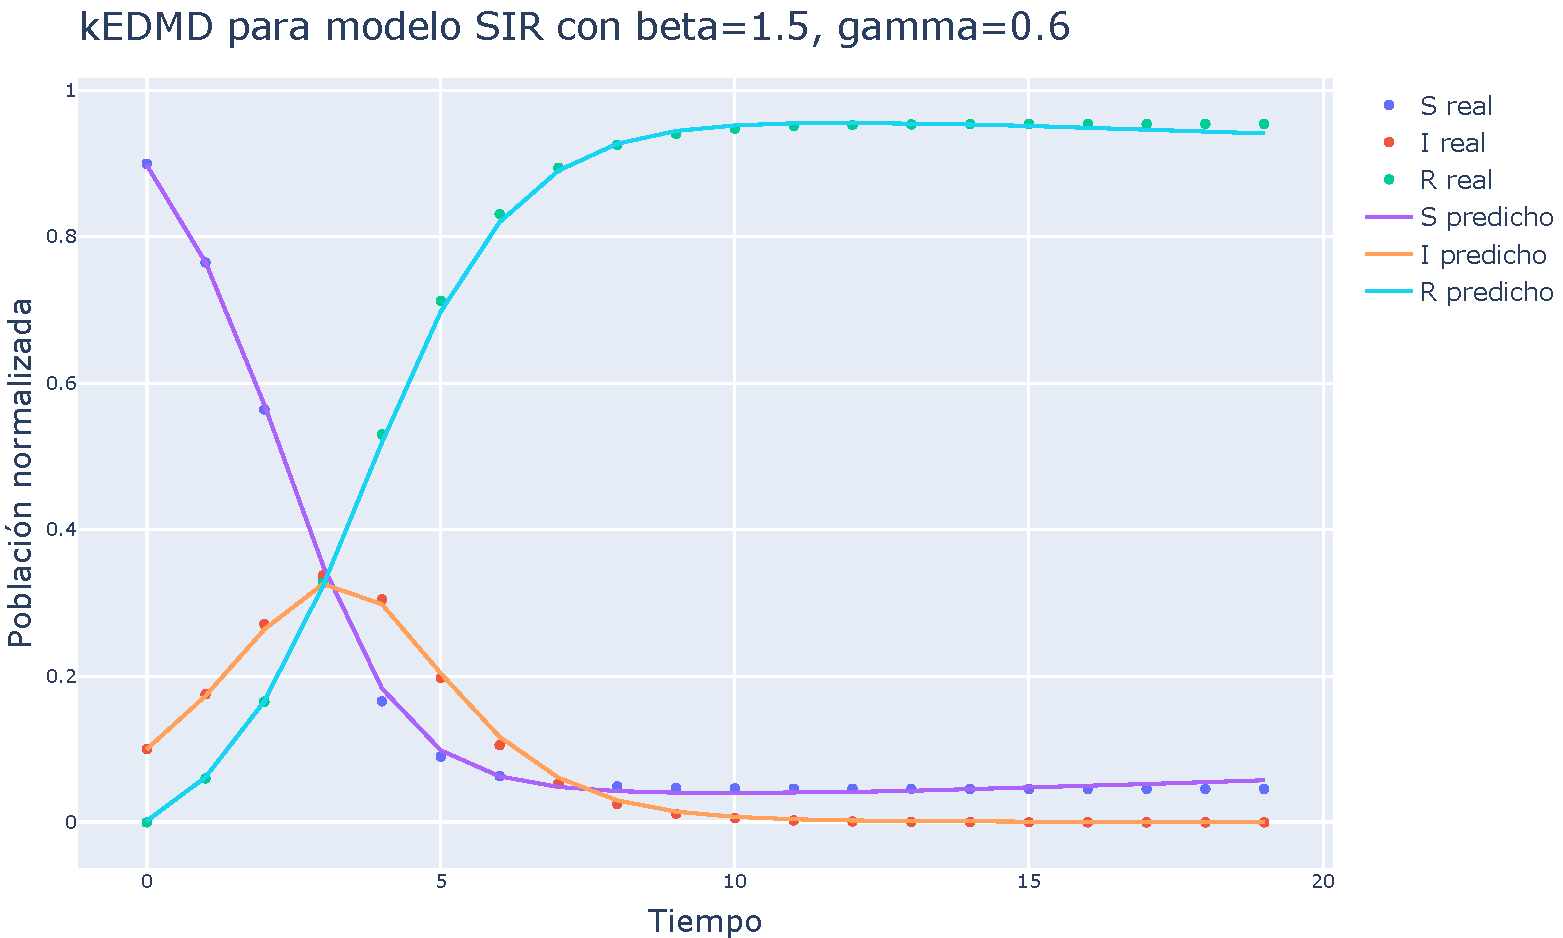
\includegraphics[width=\textwidth]{img/content/chapter3/SIR3.pdf}
        \caption{$\beta=1.5$, $\gamma = 0.6$}
    \end{subfigure}
    \caption{Ilustración de los tres casos de $\beta$ y $\gamma$ elegidos para la comparación entre el sistema no lineal original y el sistema linealizado por Koopman a 1000 puntos \textit{sampleados} de una variable aleatoria Dirichlet. En forma de puntos se dejan los valores reales que toma el sistema y en línea continua los valores entregados por el sistema linealizado, que se consideran como predicción.}
    \label{fig:Comp_traj_SIR}
\end{figure}

\begin{figure}[h]
    \centering
    \begin{subfigure}[b]{0.32\textwidth}
        \centering
        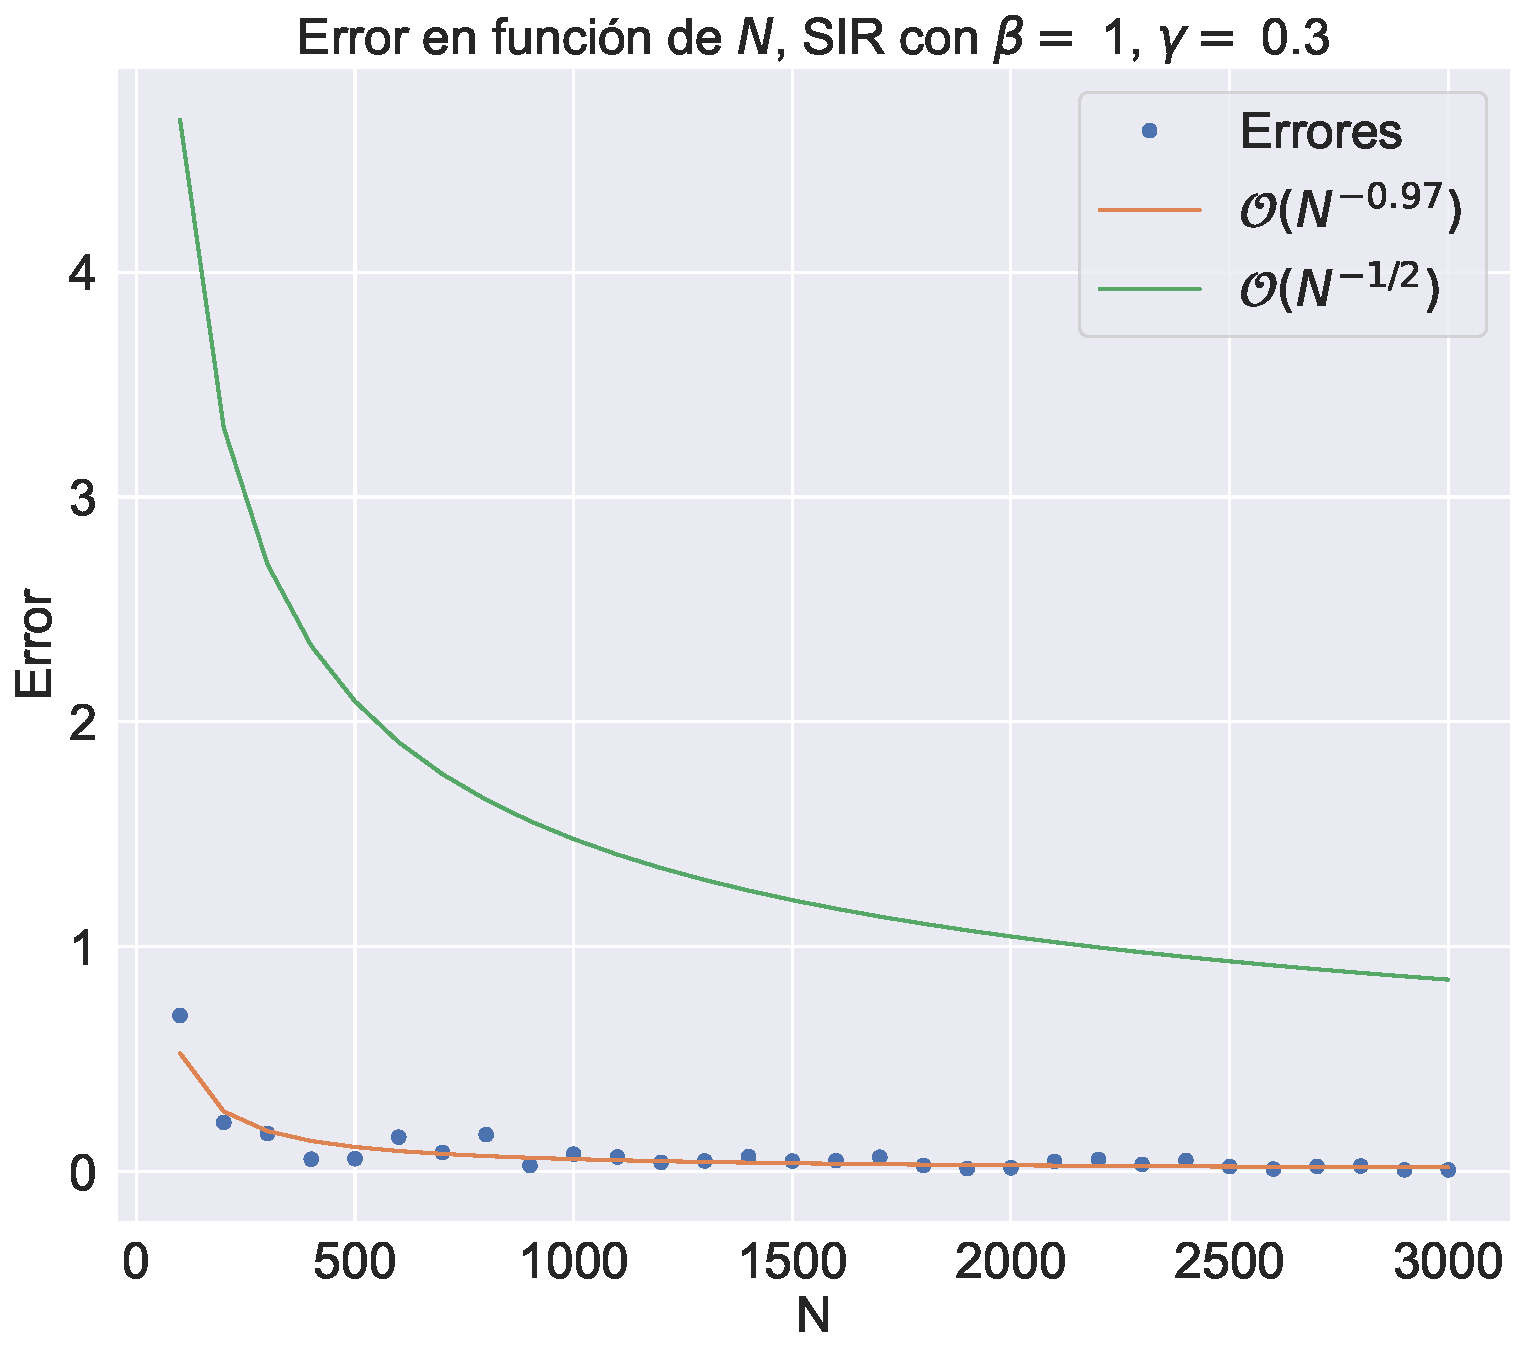
\includegraphics[width=\textwidth]{img/content/chapter3/SIR1Errors.pdf}
        \caption{$\beta=-0.3$, $\gamma=0.3$}
    \end{subfigure}
    \hfill
    \begin{subfigure}[b]{0.32\textwidth}
        \centering
        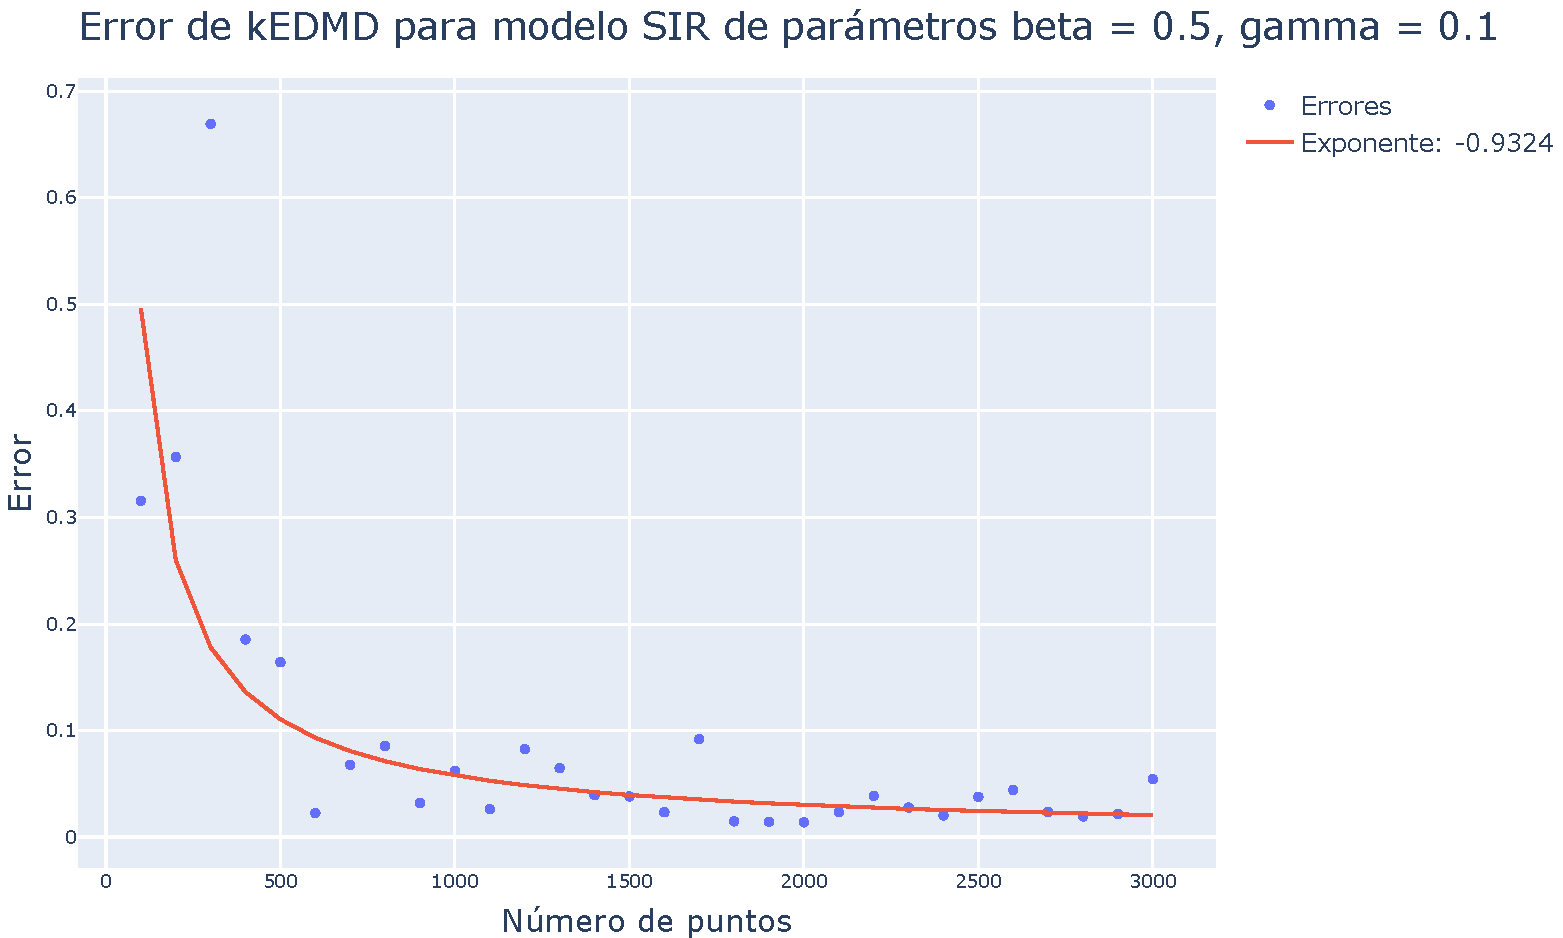
\includegraphics[width=\textwidth]{img/content/chapter3/SIR2Errors.pdf}
        \caption{$\beta=0.5$, $\gamma=0.1$}
    \end{subfigure}
    \hfill
    \begin{subfigure}[b]{0.32\textwidth}
        \centering
        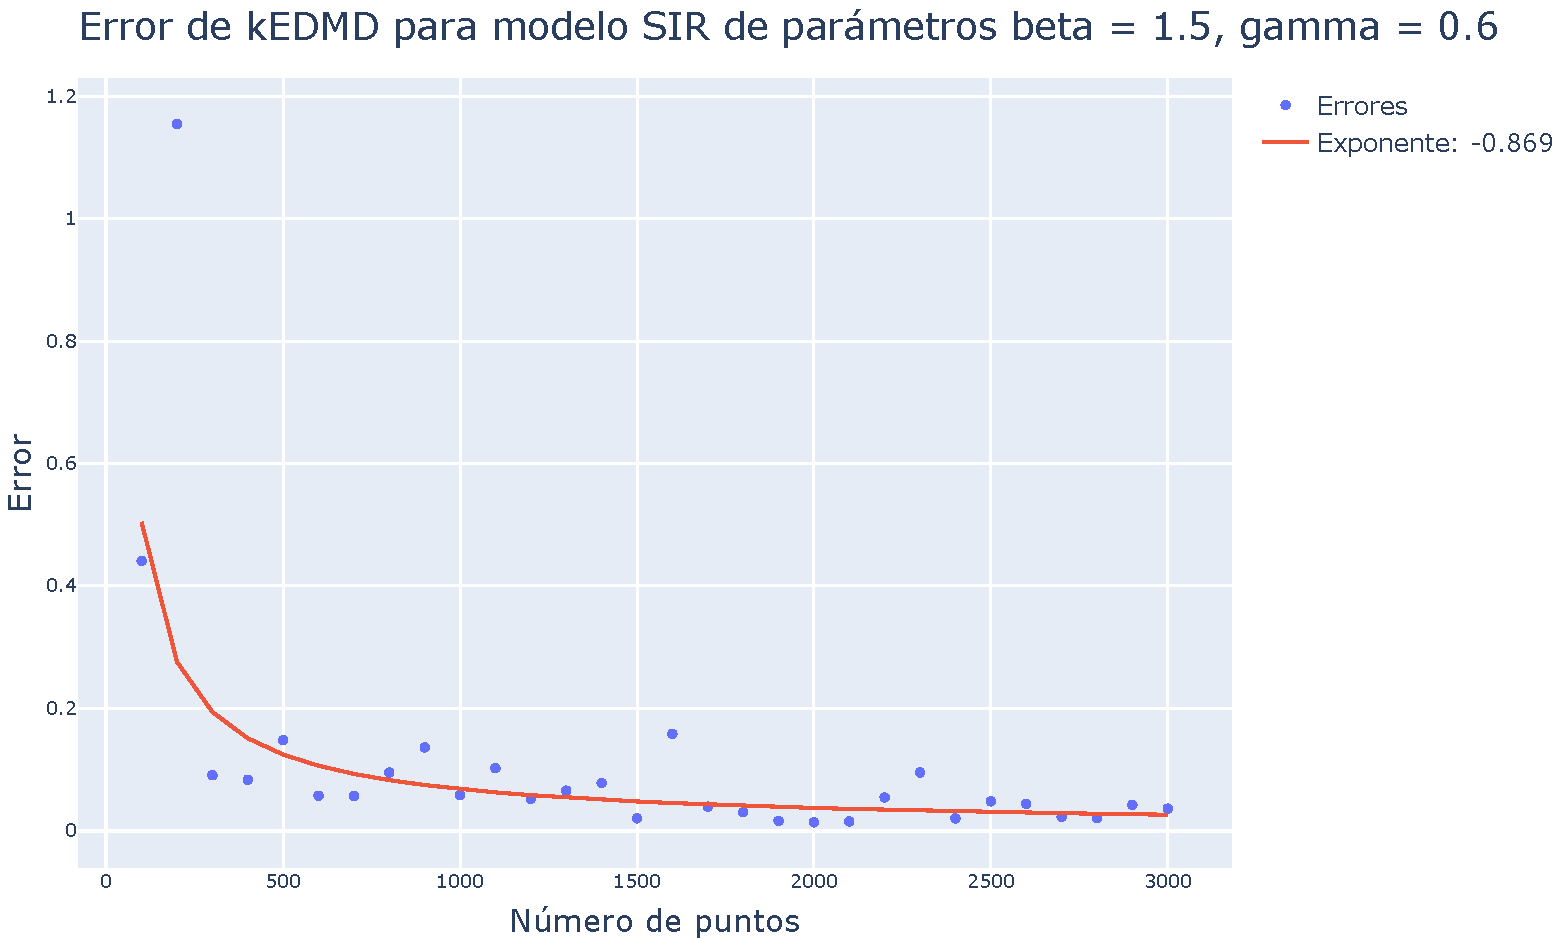
\includegraphics[width=\textwidth]{img/content/chapter3/SIR3Errors.pdf}
        \caption{$\beta=1.5$, $\gamma=0.6$}
    \end{subfigure}
    \caption{Ilustración de los tres casos del modelo SIR elegido para la evolución en función de $N$ de la diferencia en norma entre el sistema lineal original y el sistema linealizado por Koopman a $N$ puntos,  \textit{sampleados} de una variable aleatoria normal. En forma de puntos se deja la evolución observada del error y en línea continua la mejor curva de la forma $C \cdot N^{a}$, donde $a$ es el exponente que se deja en la leyenda.}
    \label{fig:ErrorSIR}
\end{figure}

\begin{figure}[h]
    \centering
    \begin{subfigure}[b]{0.45\textwidth}
        \centering
        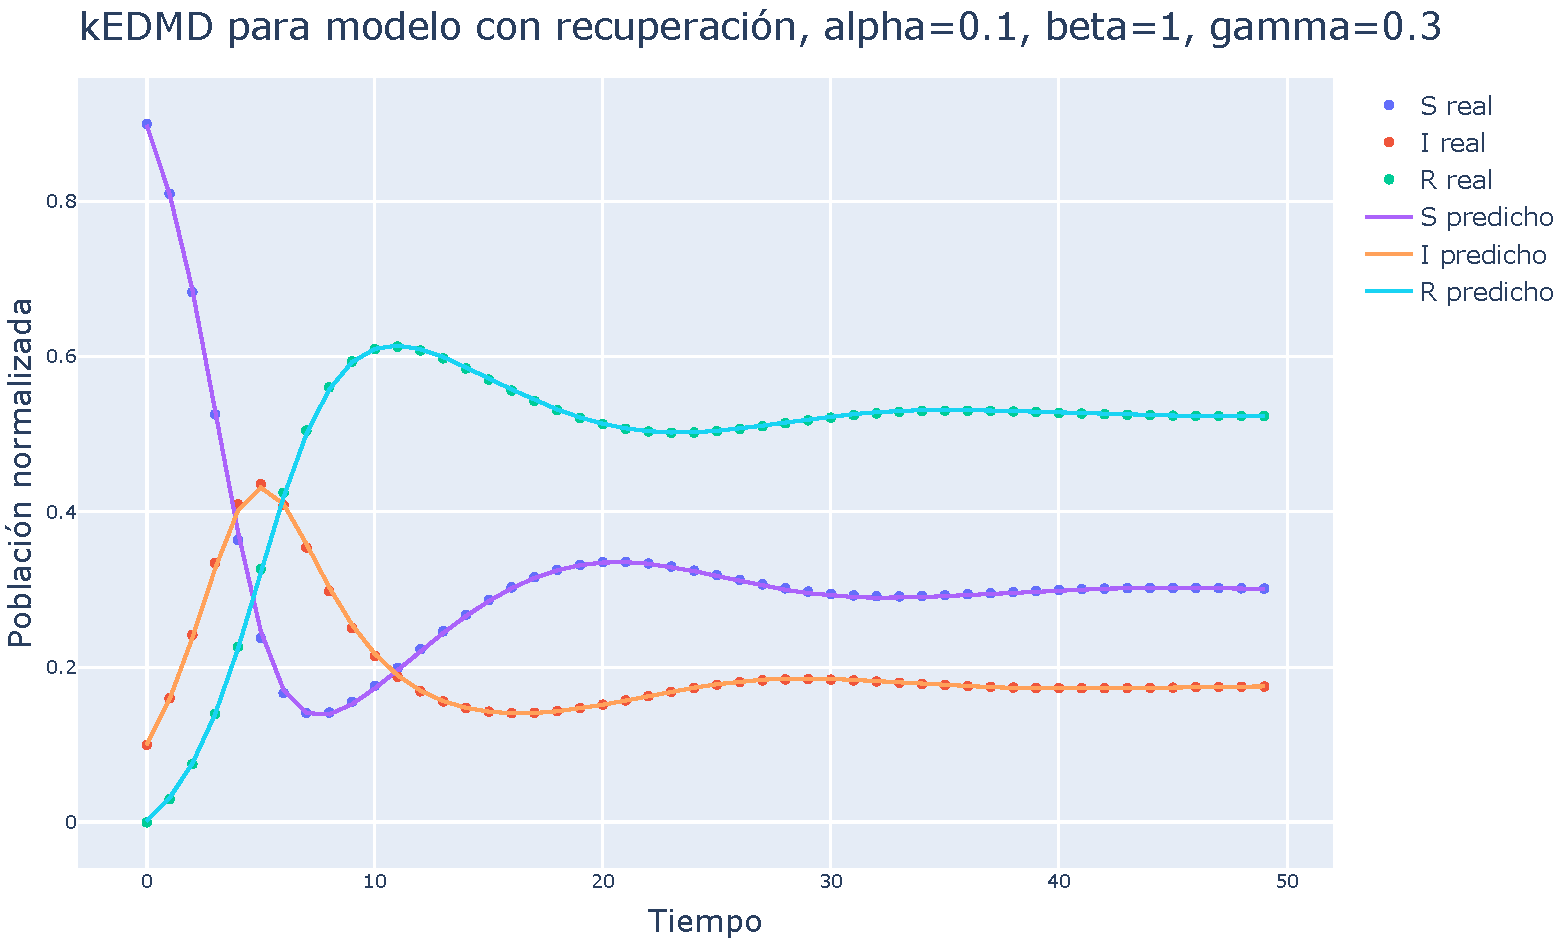
\includegraphics[width=\textwidth]{img/content/chapter3/SIR_rec1.pdf}
        \caption{$\alpha=-0.3$}
        \label{fig:image1}
    \end{subfigure}
    \hfill
    \begin{subfigure}[b]{0.45\textwidth}
        \centering
        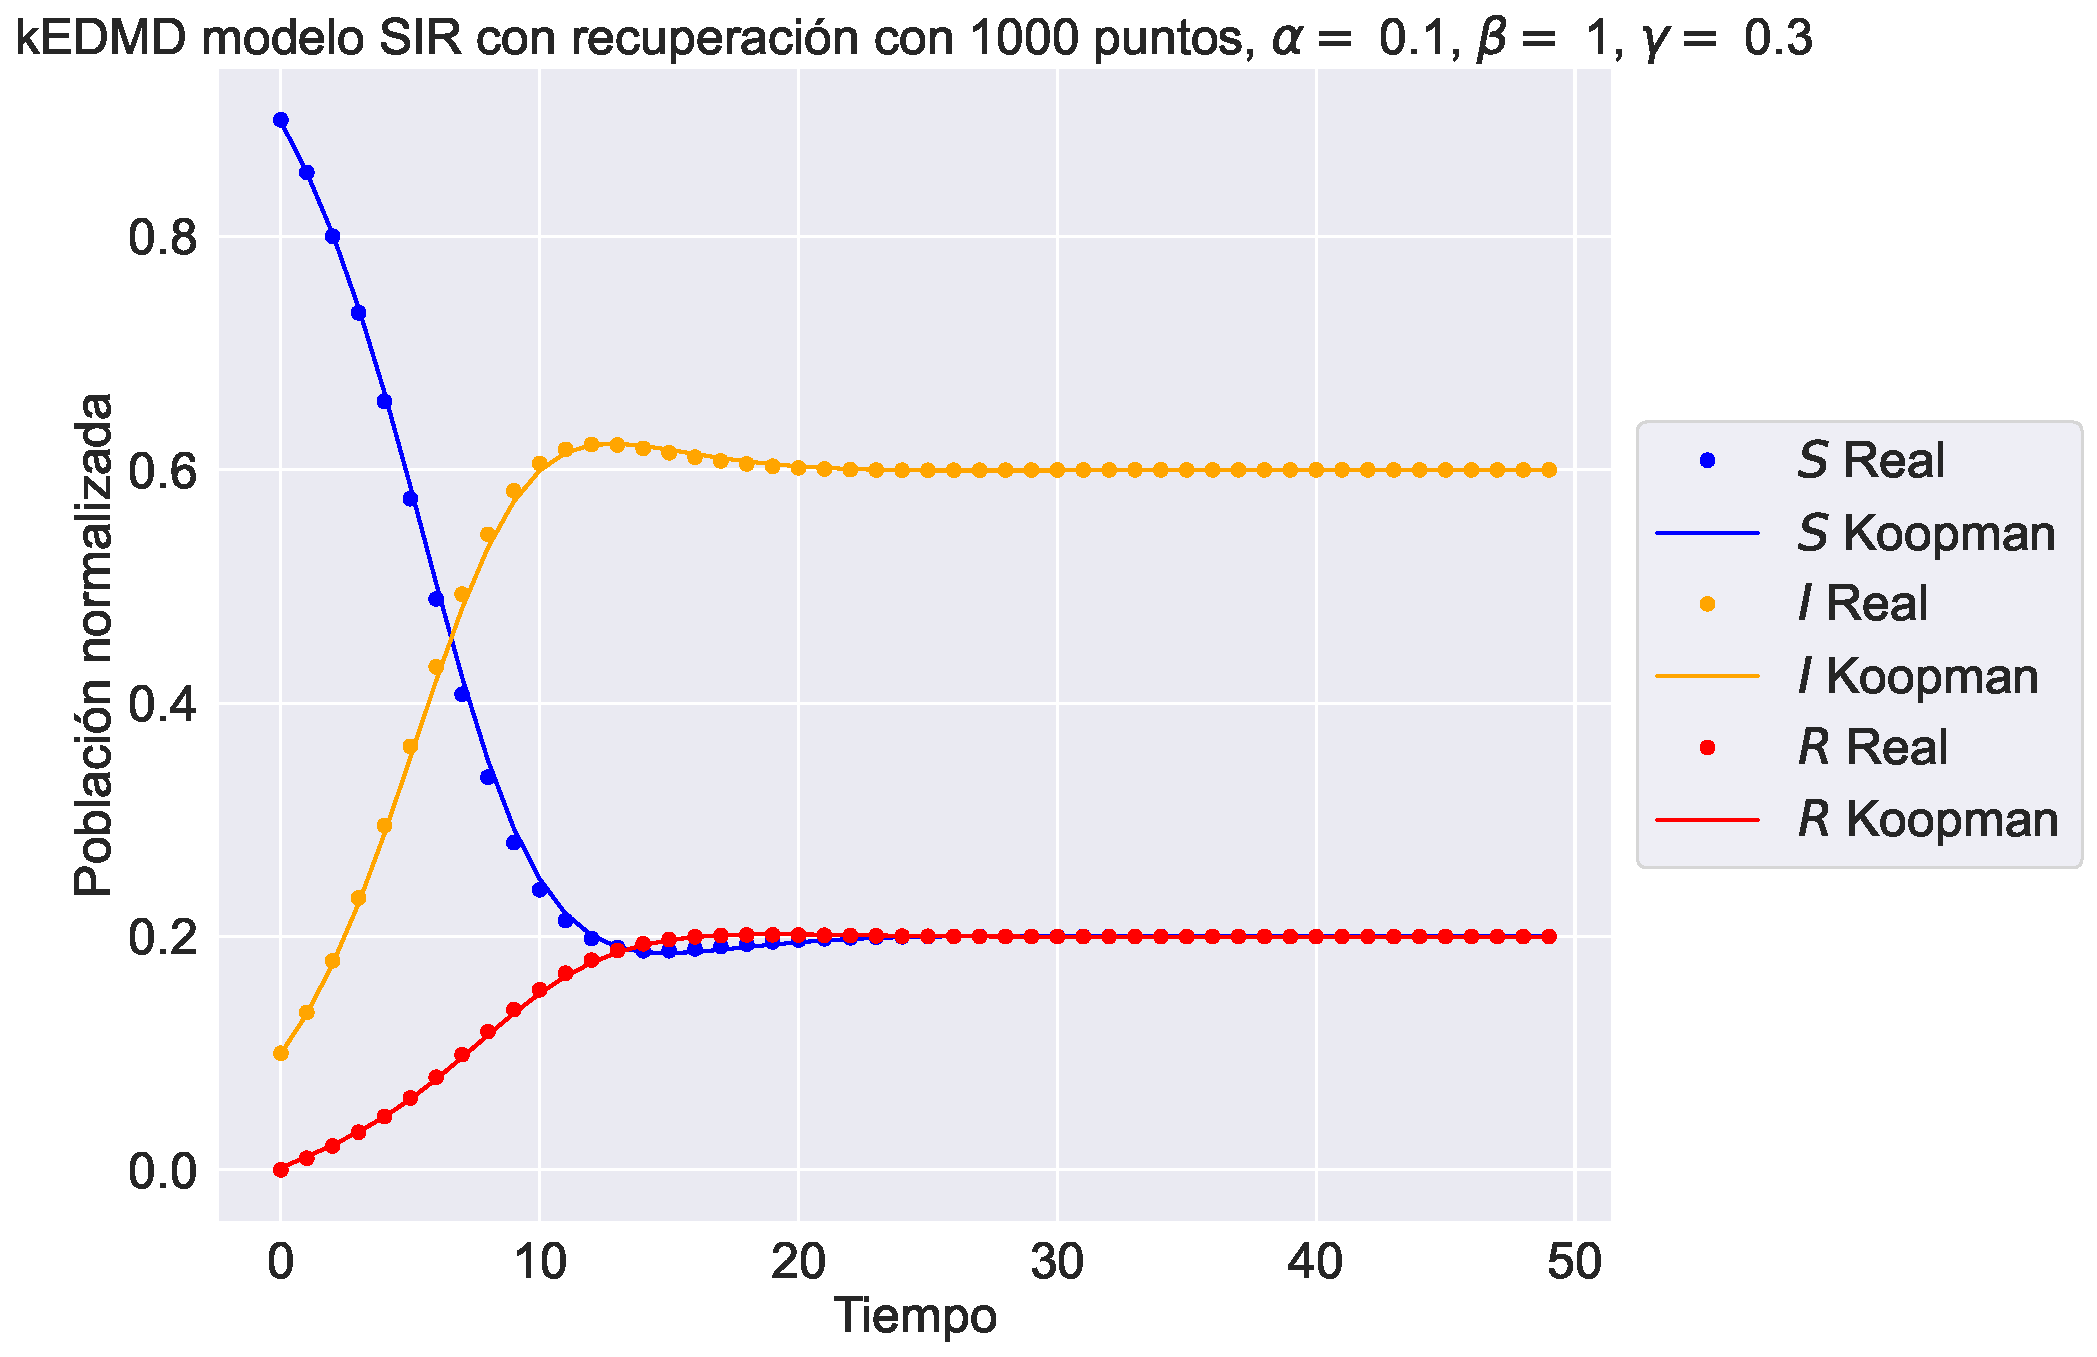
\includegraphics[width=\textwidth]{img/content/chapter3/SIR_rec2.pdf}
        \caption{$\alpha=-0.1$}
        \label{fig:image2}
    \end{subfigure}
    \hfill
    \begin{subfigure}[b]{0.45\textwidth}
        \centering
        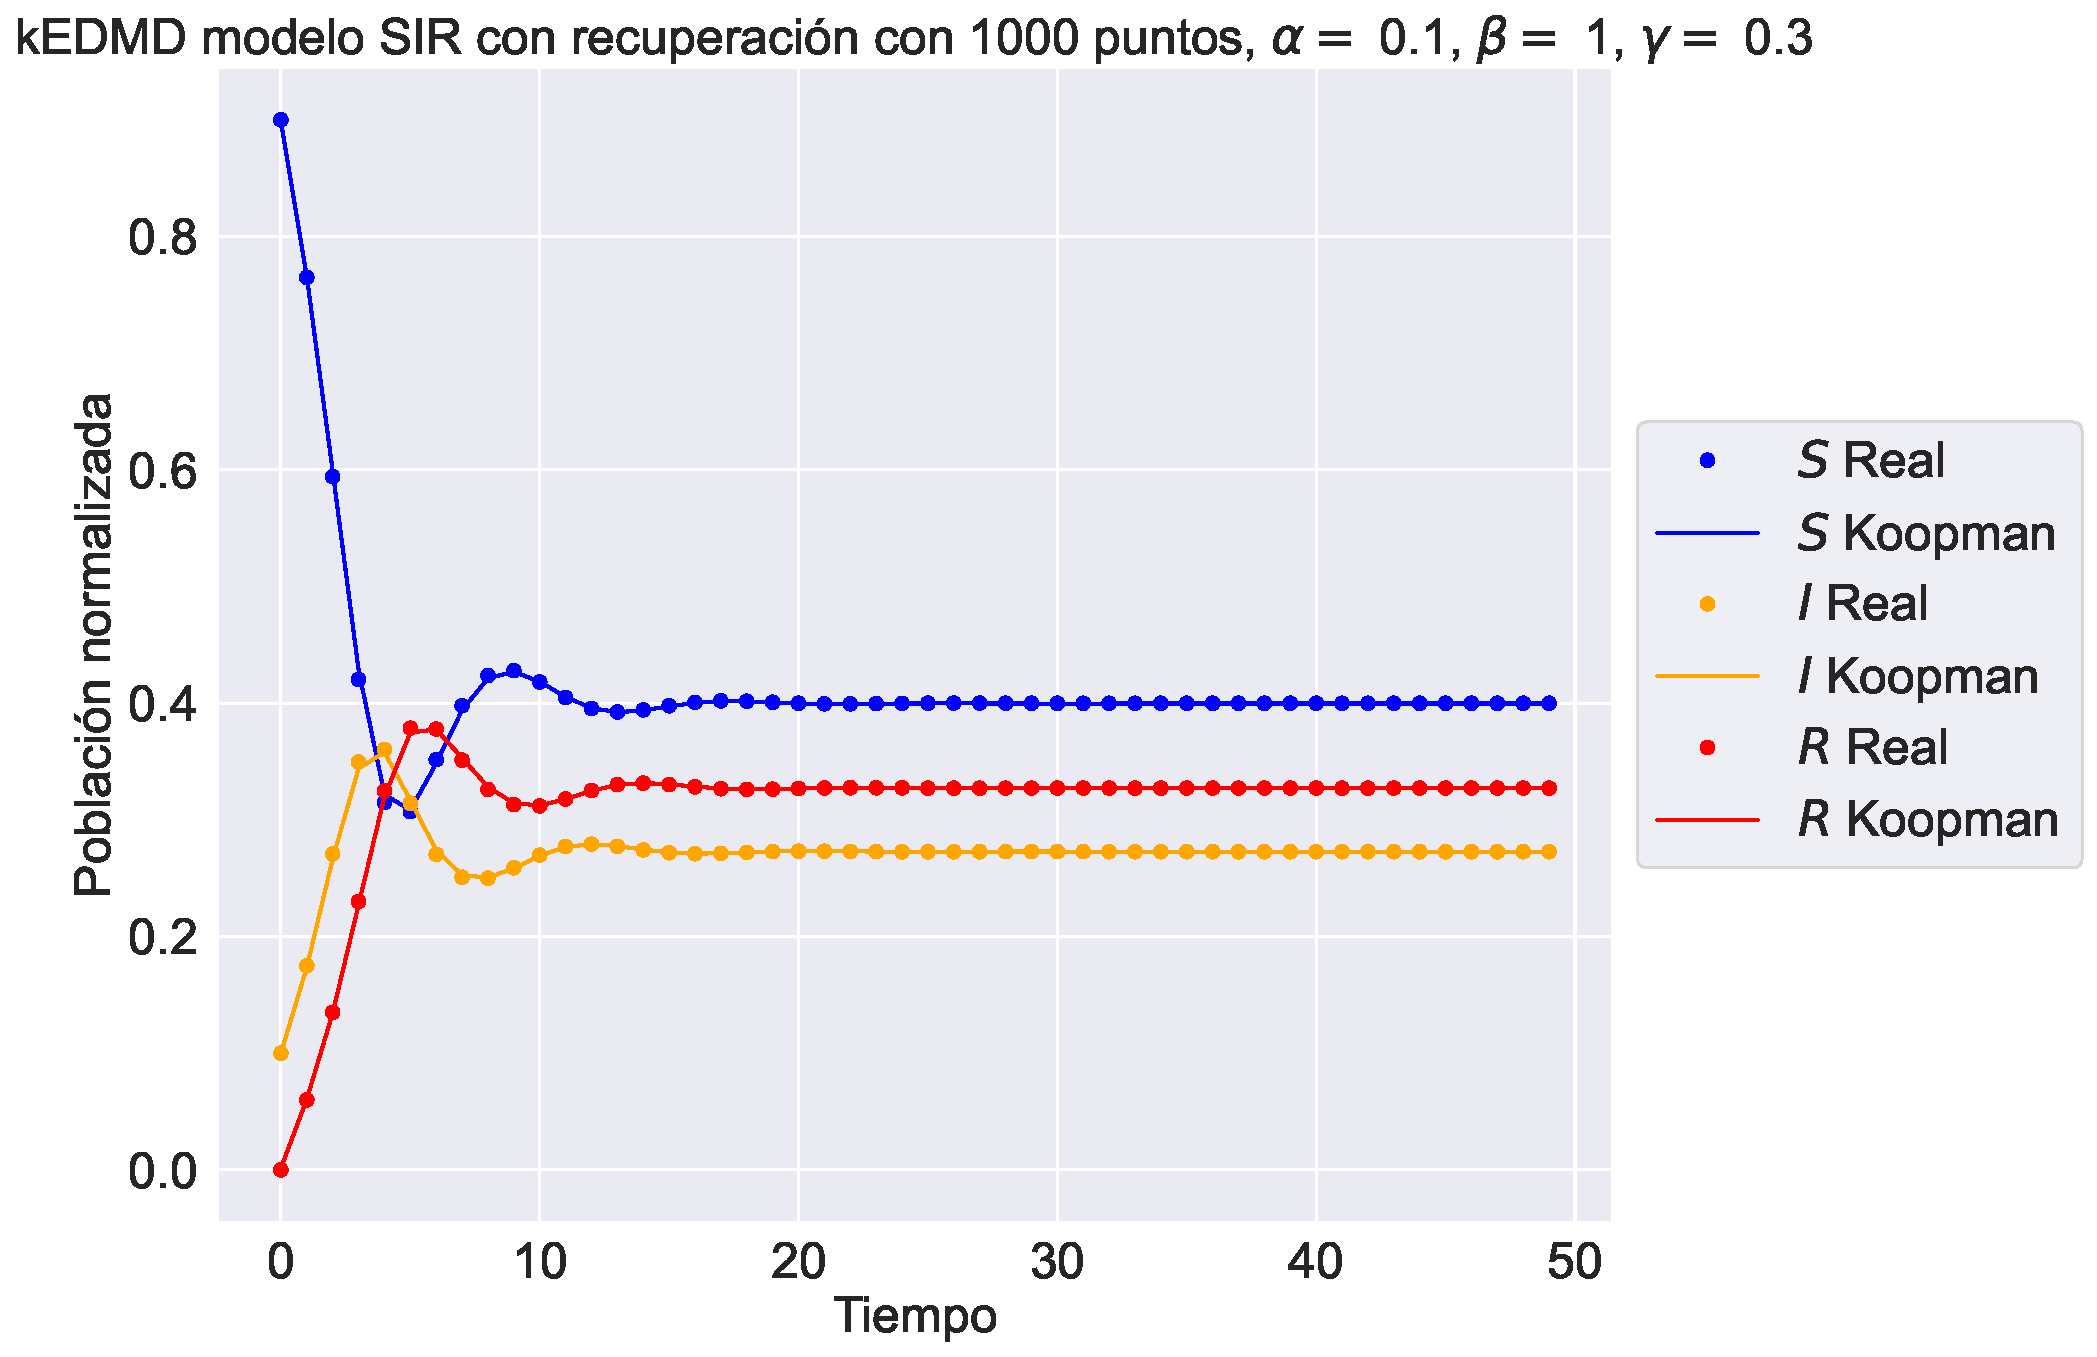
\includegraphics[width=\textwidth]{img/content/chapter3/SIR_rec3.pdf}
        \caption{$\alpha=0.05$}
    \end{subfigure}
    \caption{Ilustración de los tres casos de $\beta$ y $\gamma$ elegidos para la comparación entre el sistema no lineal original y el sistema linealizado por Koopman a 1000 puntos \textit{sampleados} de una variable aleatoria Dirichlet. En forma de puntos se dejan los valores reales que toma el sistema y en línea continua los valores entregados por el sistema linealizado, que se consideran como predicción.}
    \label{fig:Comp_traj_SIR}
\end{figure}
\begin{figure}[h]
    \centering
    \begin{subfigure}[b]{0.32\textwidth}
        \centering
        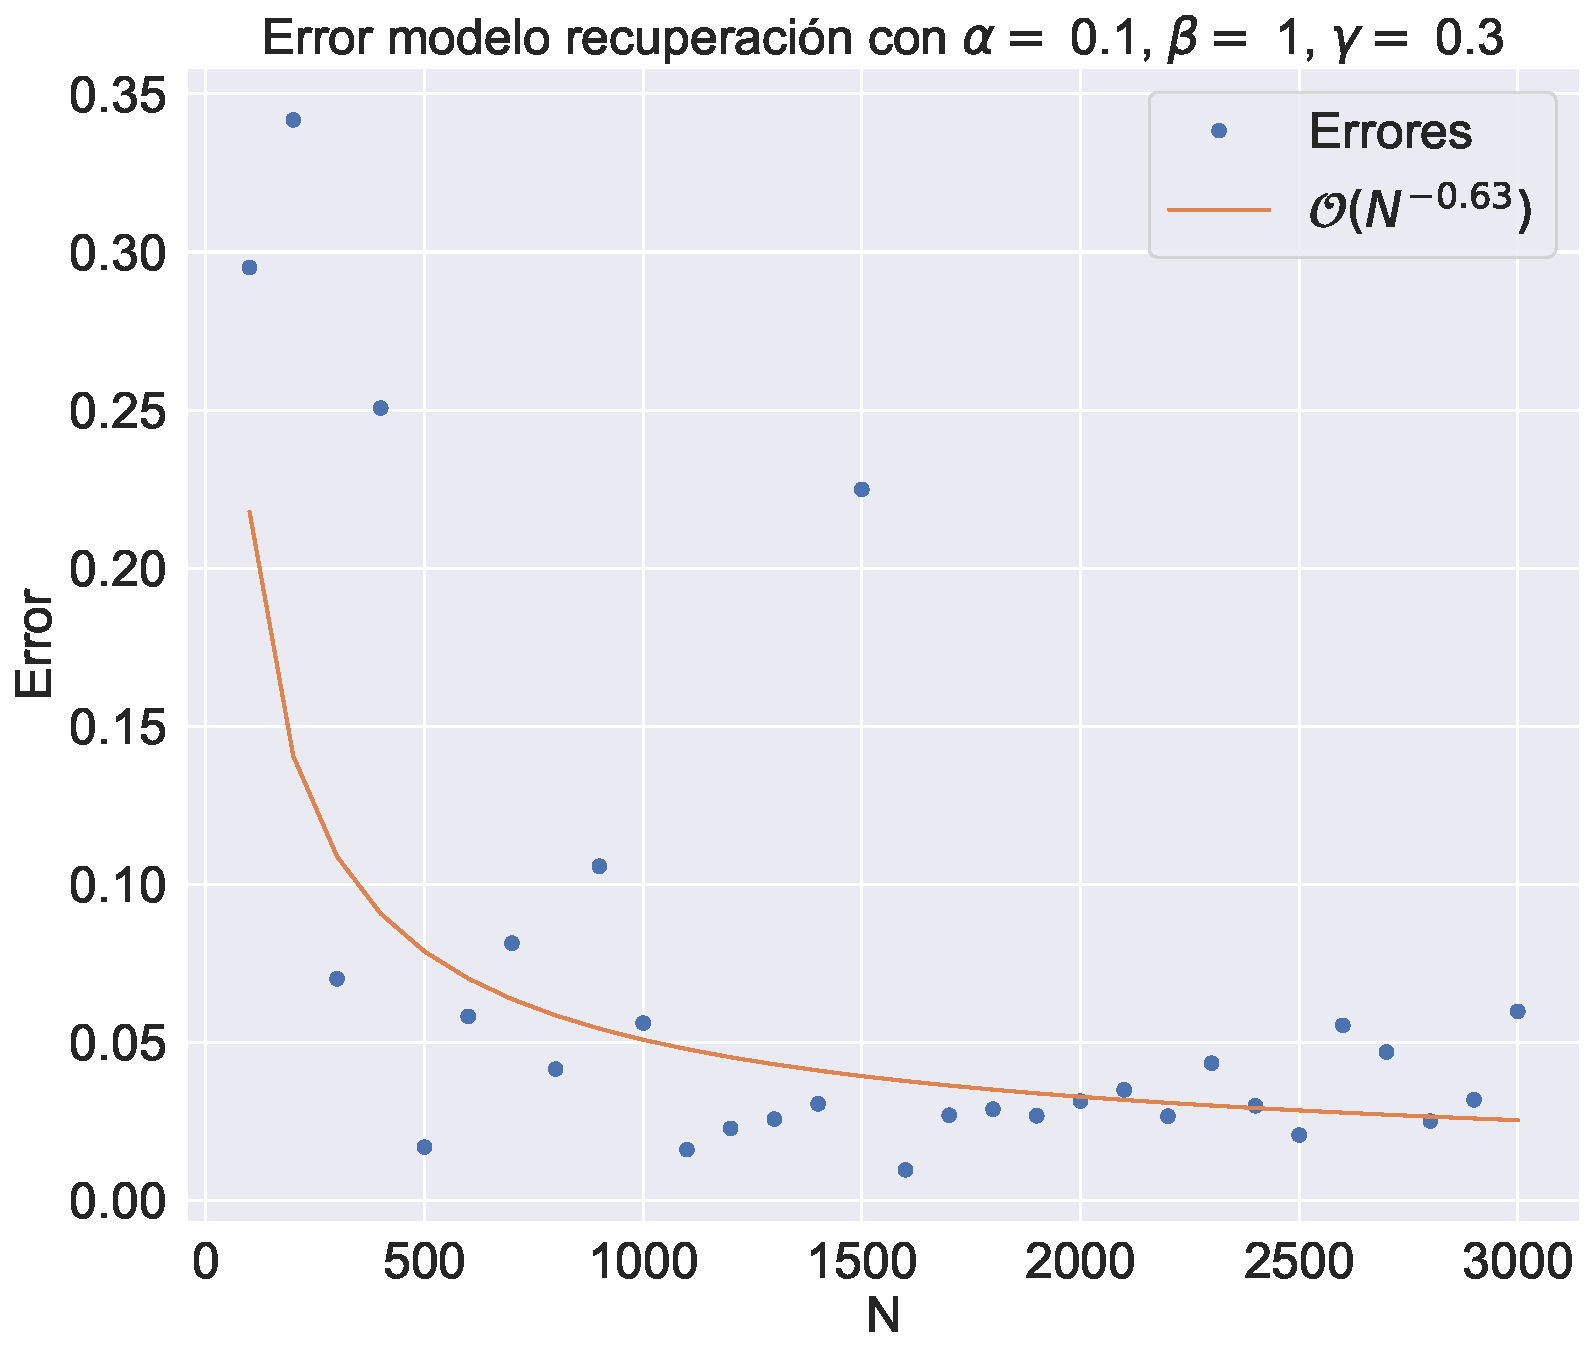
\includegraphics[width=\textwidth]{img/content/chapter3/SIR_rec1Errors.pdf}
        \caption{$\alpha=0.1$, $\beta=1$, $\gamma=0.3$}
    \end{subfigure}
    \hfill
    \begin{subfigure}[b]{0.32\textwidth}
        \centering
        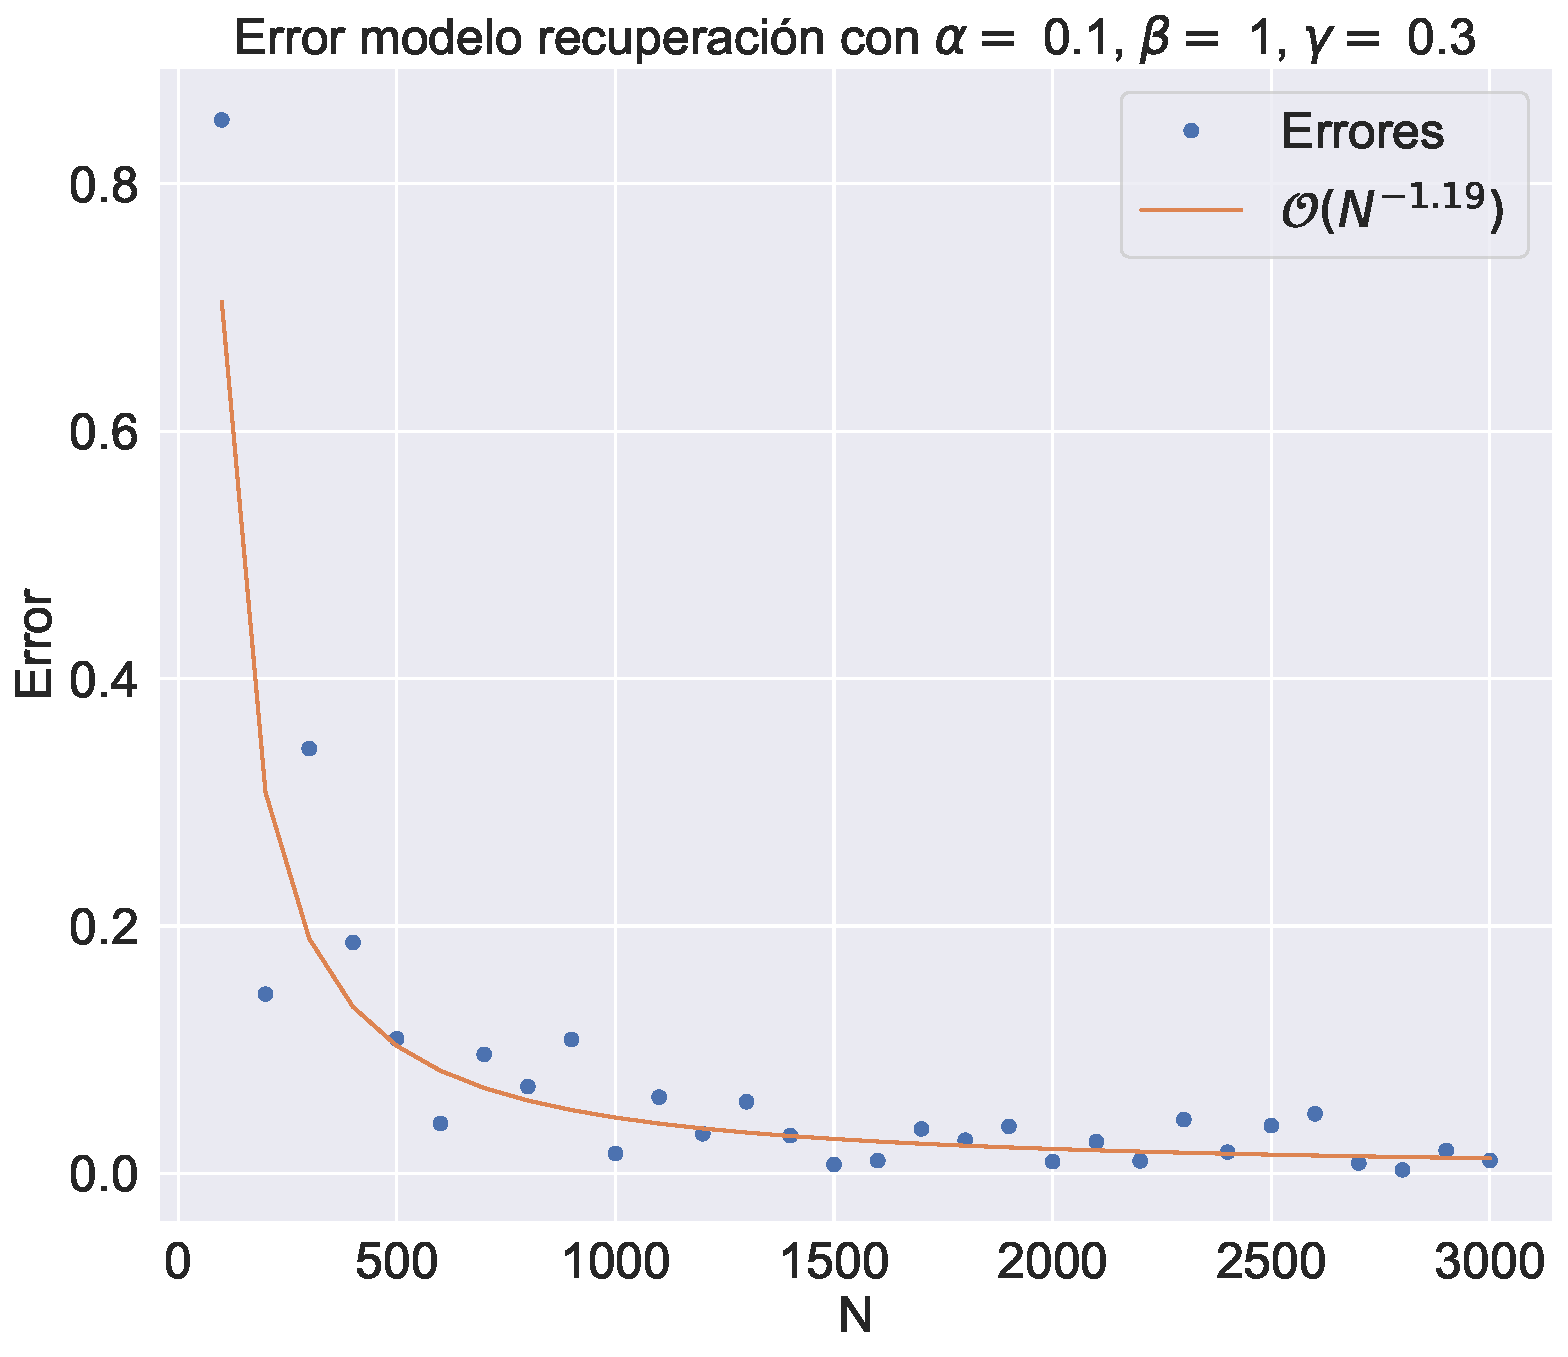
\includegraphics[width=\textwidth]{img/content/chapter3/SIR_rec2Errors.pdf}
        \caption{$\alpha=0.3$, $\beta=1$, $\gamma=0.3$}
    \end{subfigure}
    \hfill
    \begin{subfigure}[b]{0.32\textwidth}
        \centering
        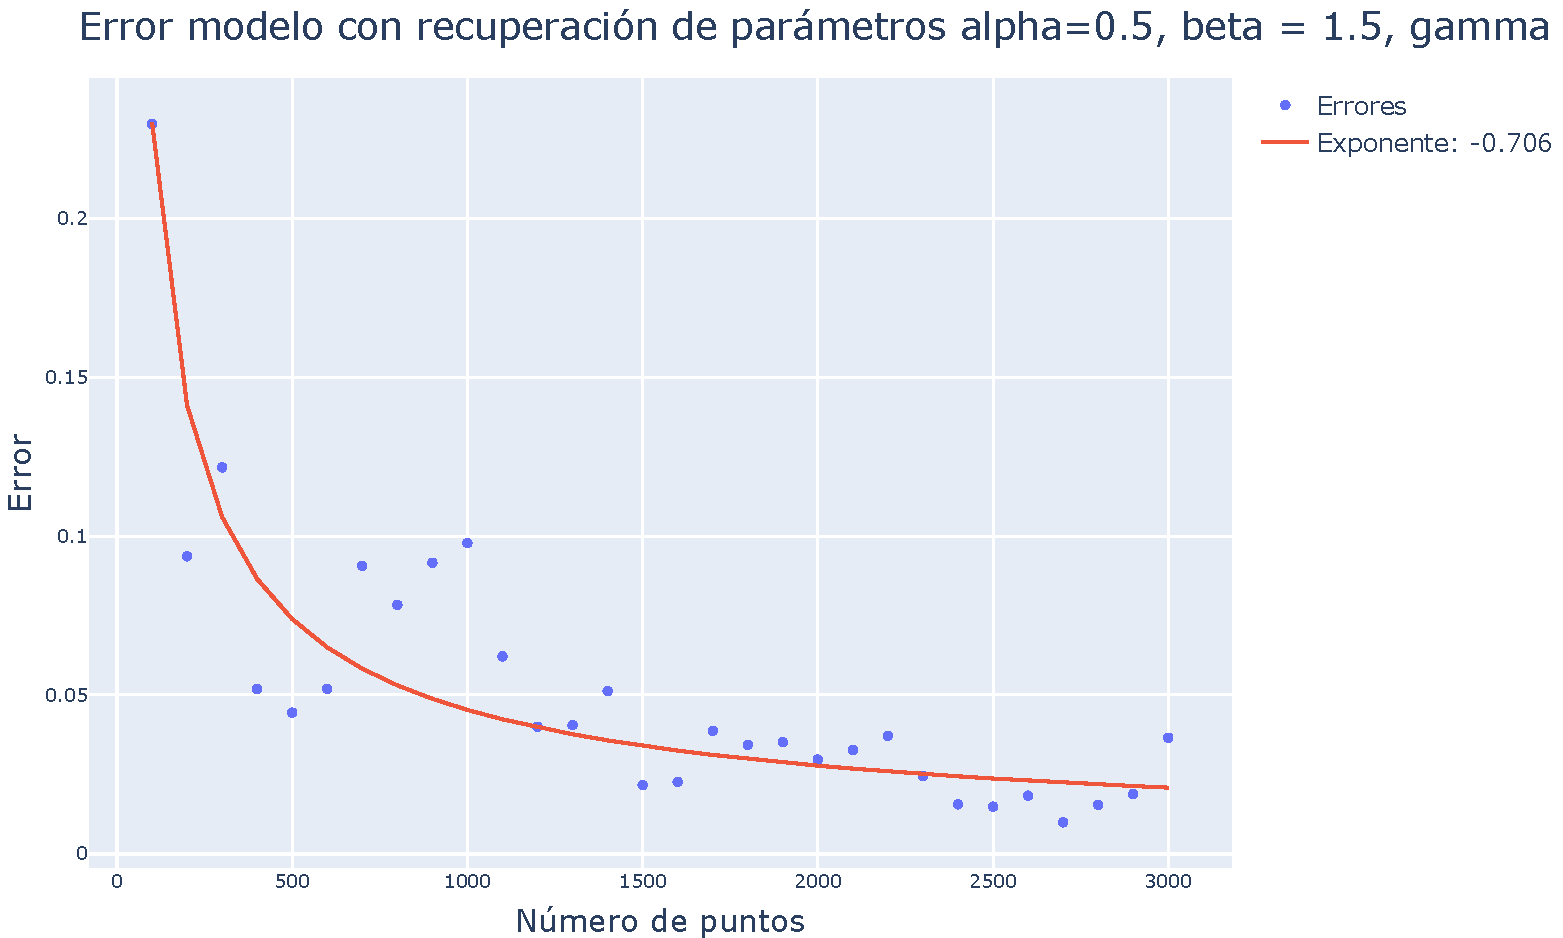
\includegraphics[width=\textwidth]{img/content/chapter3/SIR_rec3Errors.pdf}
        \caption{$\alpha=0.05$}
    \end{subfigure}
    \caption{Ilustración de los tres casos del modelo SIR con pérdida de inmunidad elegido para la evolución en función de $N$ de la diferencia en norma entre el sistema lineal original y el sistema linealizado por Koopman a $N$ puntos,  \textit{sampleados} de una variable aleatoria normal. En forma de puntos se deja la evolución observada del error y en línea continua la mejor curva de la forma $C \cdot N^{a}$, donde $a$ es el exponente que se deja en la leyenda.}
    \label{fig:ErrorSIR_rec}
\end{figure}


\chapter{Resultados numéricos capítulo 4}

\section{Comparación con el Filtro de Kalman}

\begin{figure}[h!]
    \centering
    \begin{subfigure}[b]{0.49\textwidth}
        \centering
        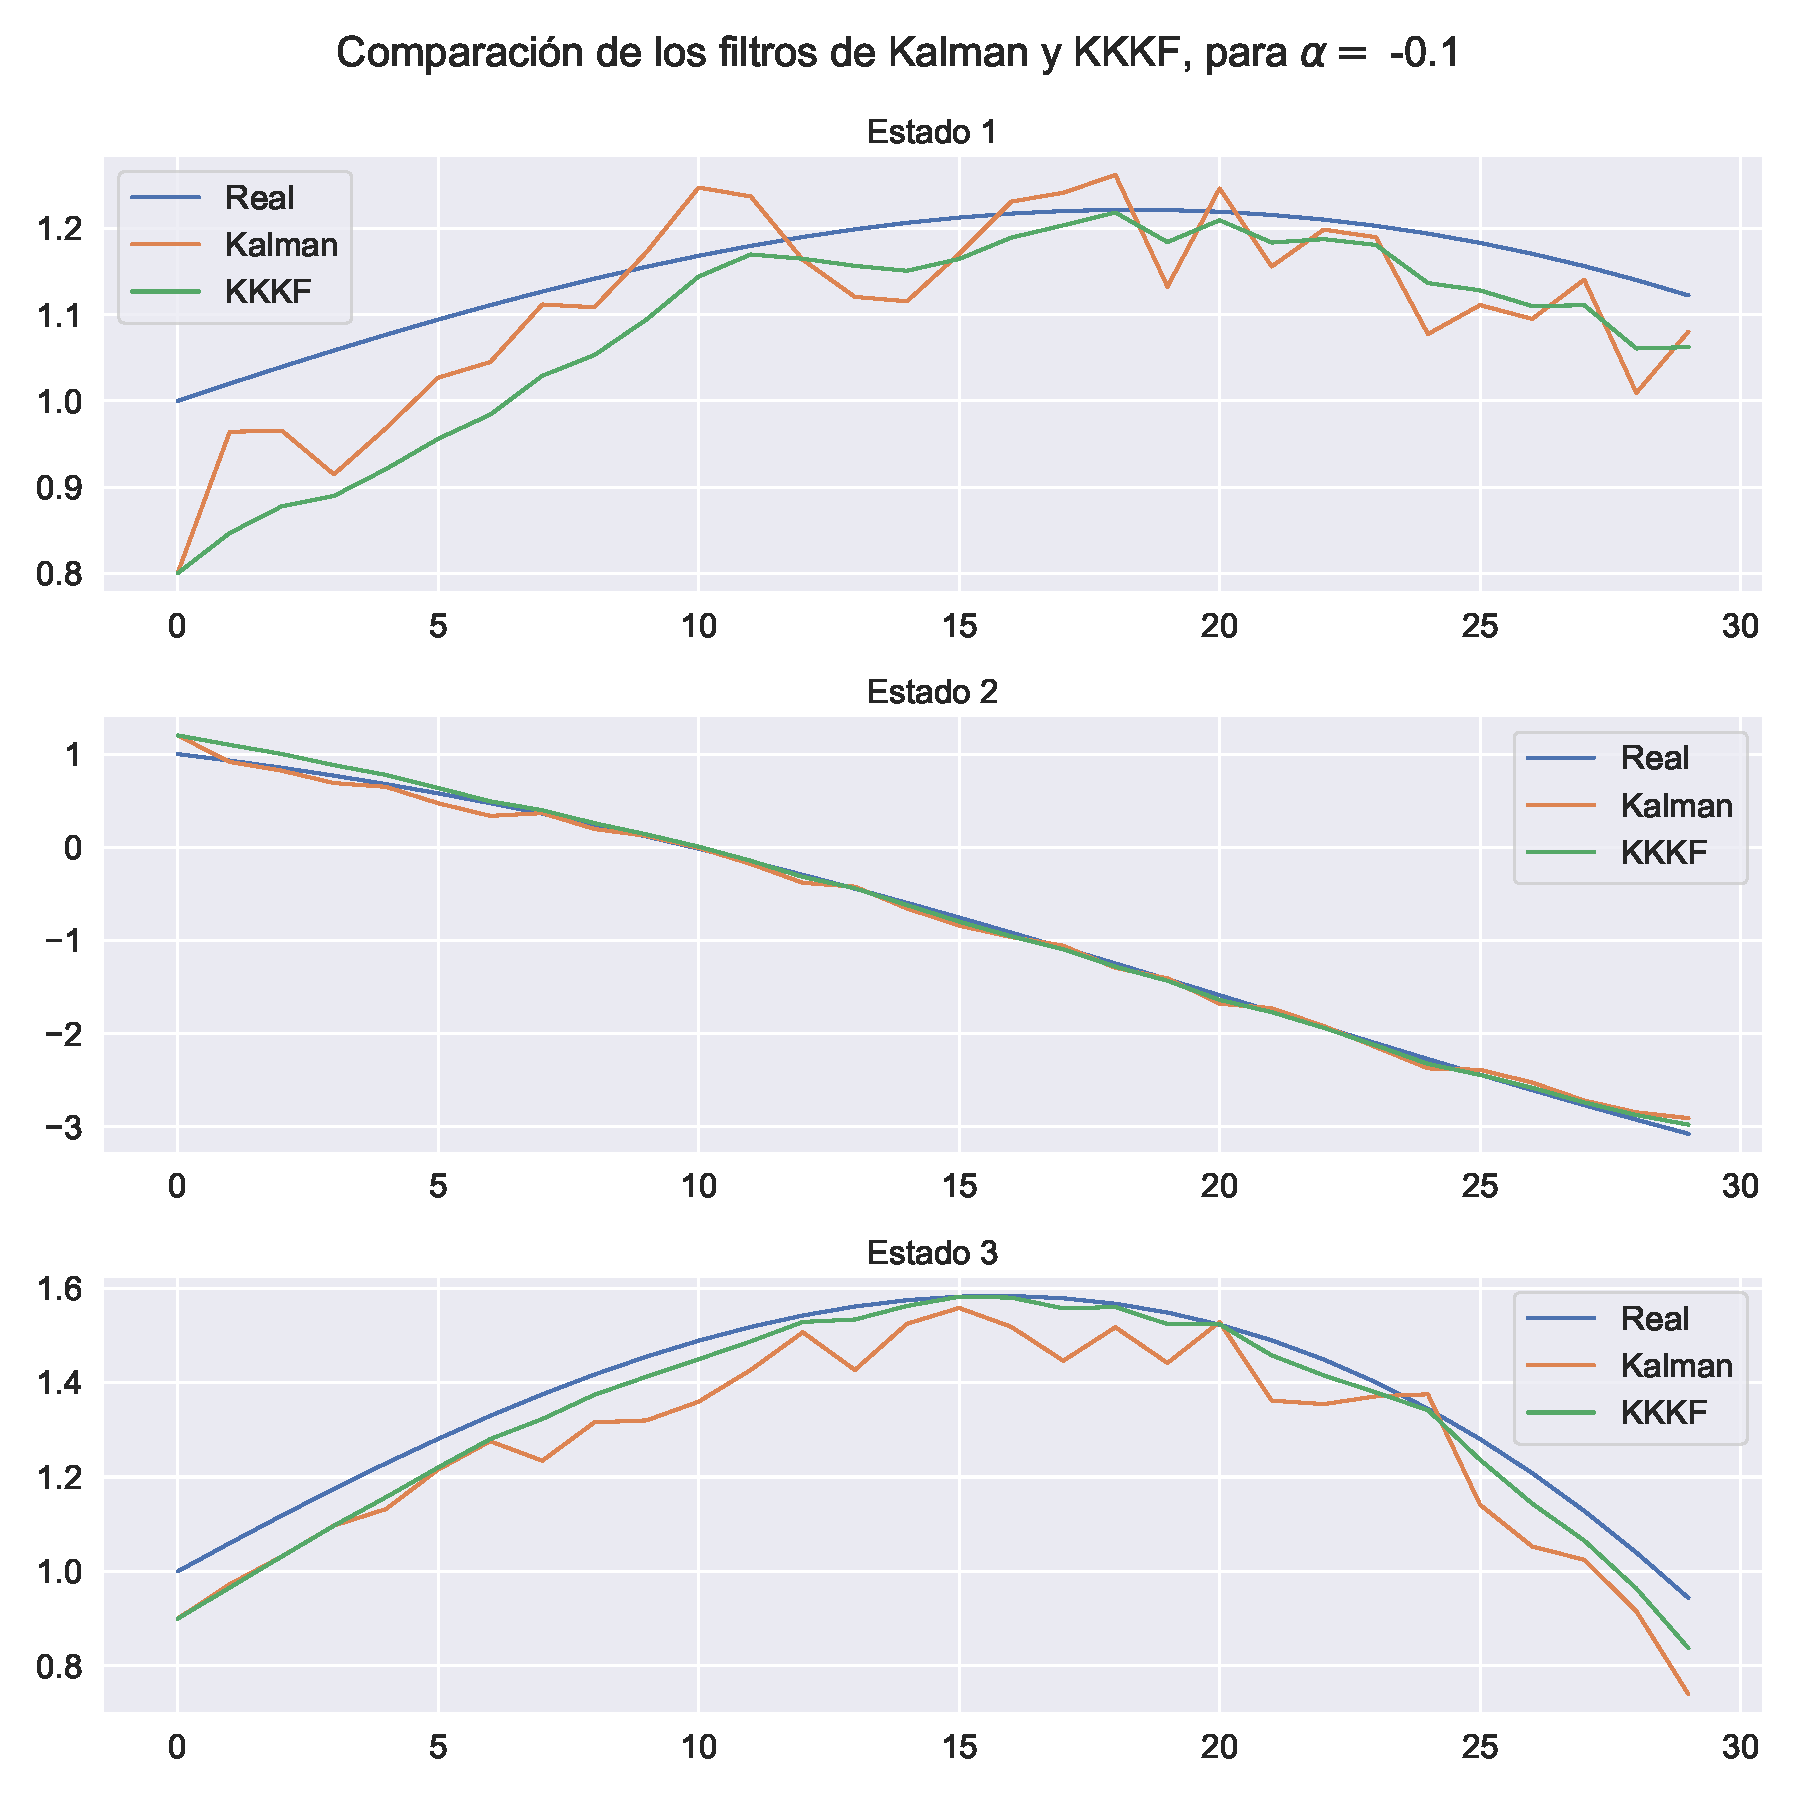
\includegraphics[width=0.75\linewidth]{img/content/chapter4/kalman_vs_kerKKF_01.pdf}
    \caption{$\alpha = -0.1$.}
    \label{fig:kalman_vs_kerKKF_01}
    \end{subfigure}
    \begin{subfigure}[b]{0.49\textwidth}
        \centering 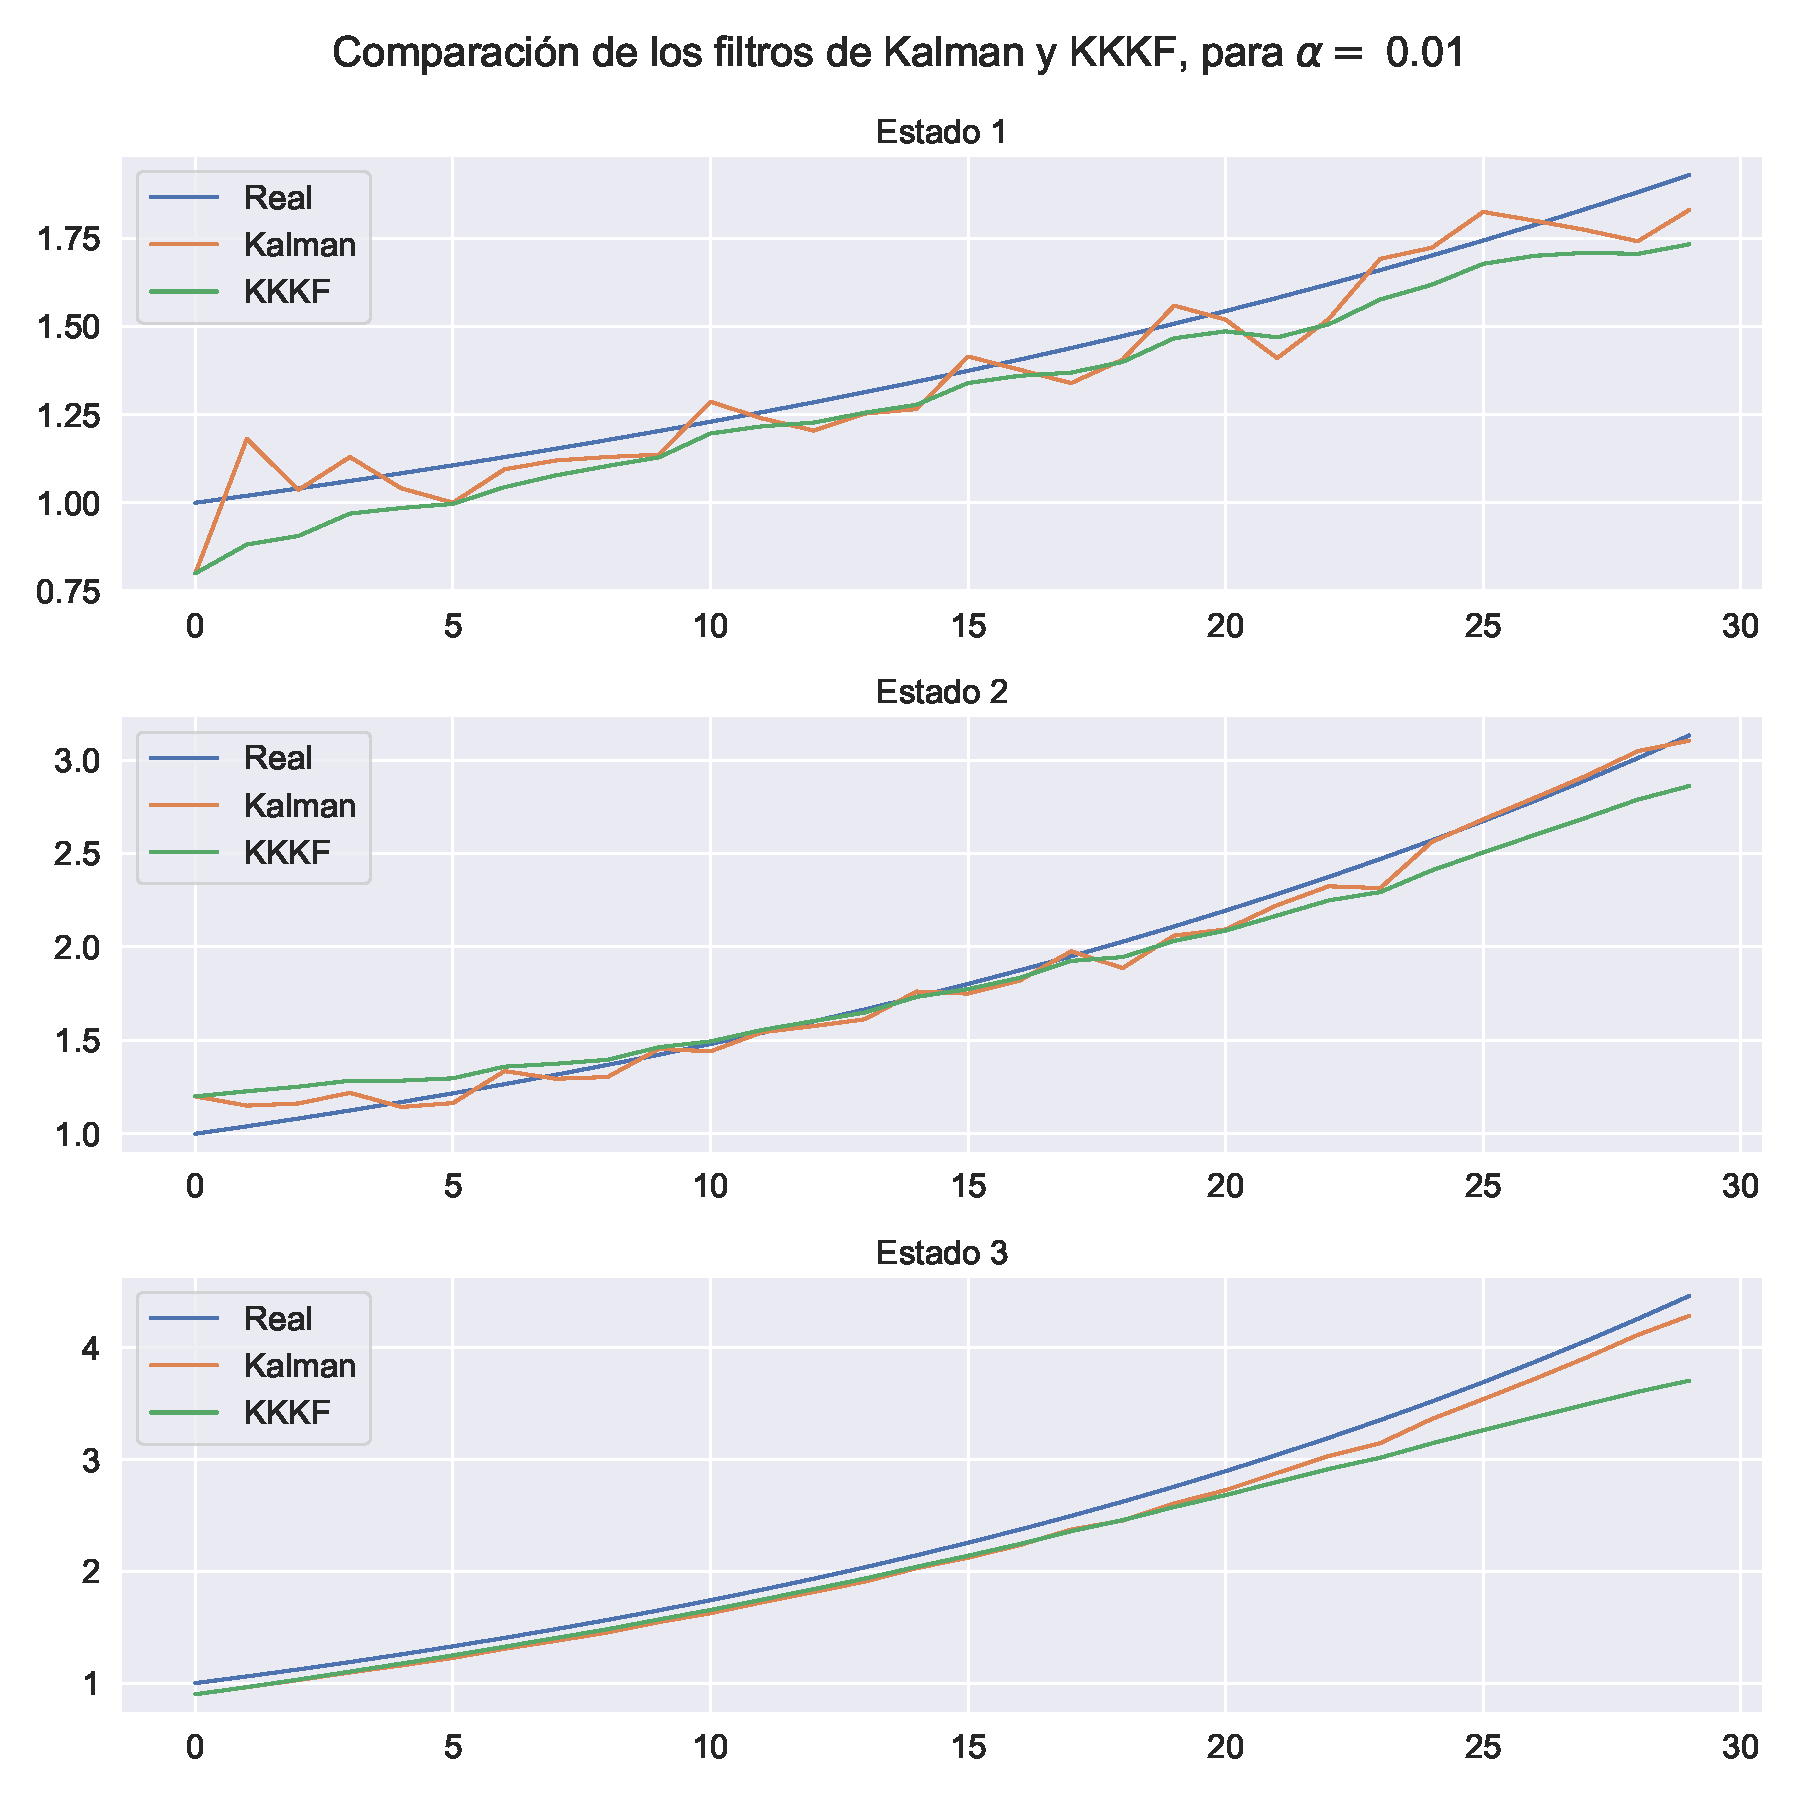
\includegraphics[width=0.75\linewidth]{img/content/chapter4/kalman_vs_kerKKF_001.pdf}
    \caption{$\alpha = 0.01$.}
    \label{fig:kalman_vs_kerKKF_001}
    \end{subfigure}
    \begin{subfigure}[b]{0.49\textwidth}
        \centering 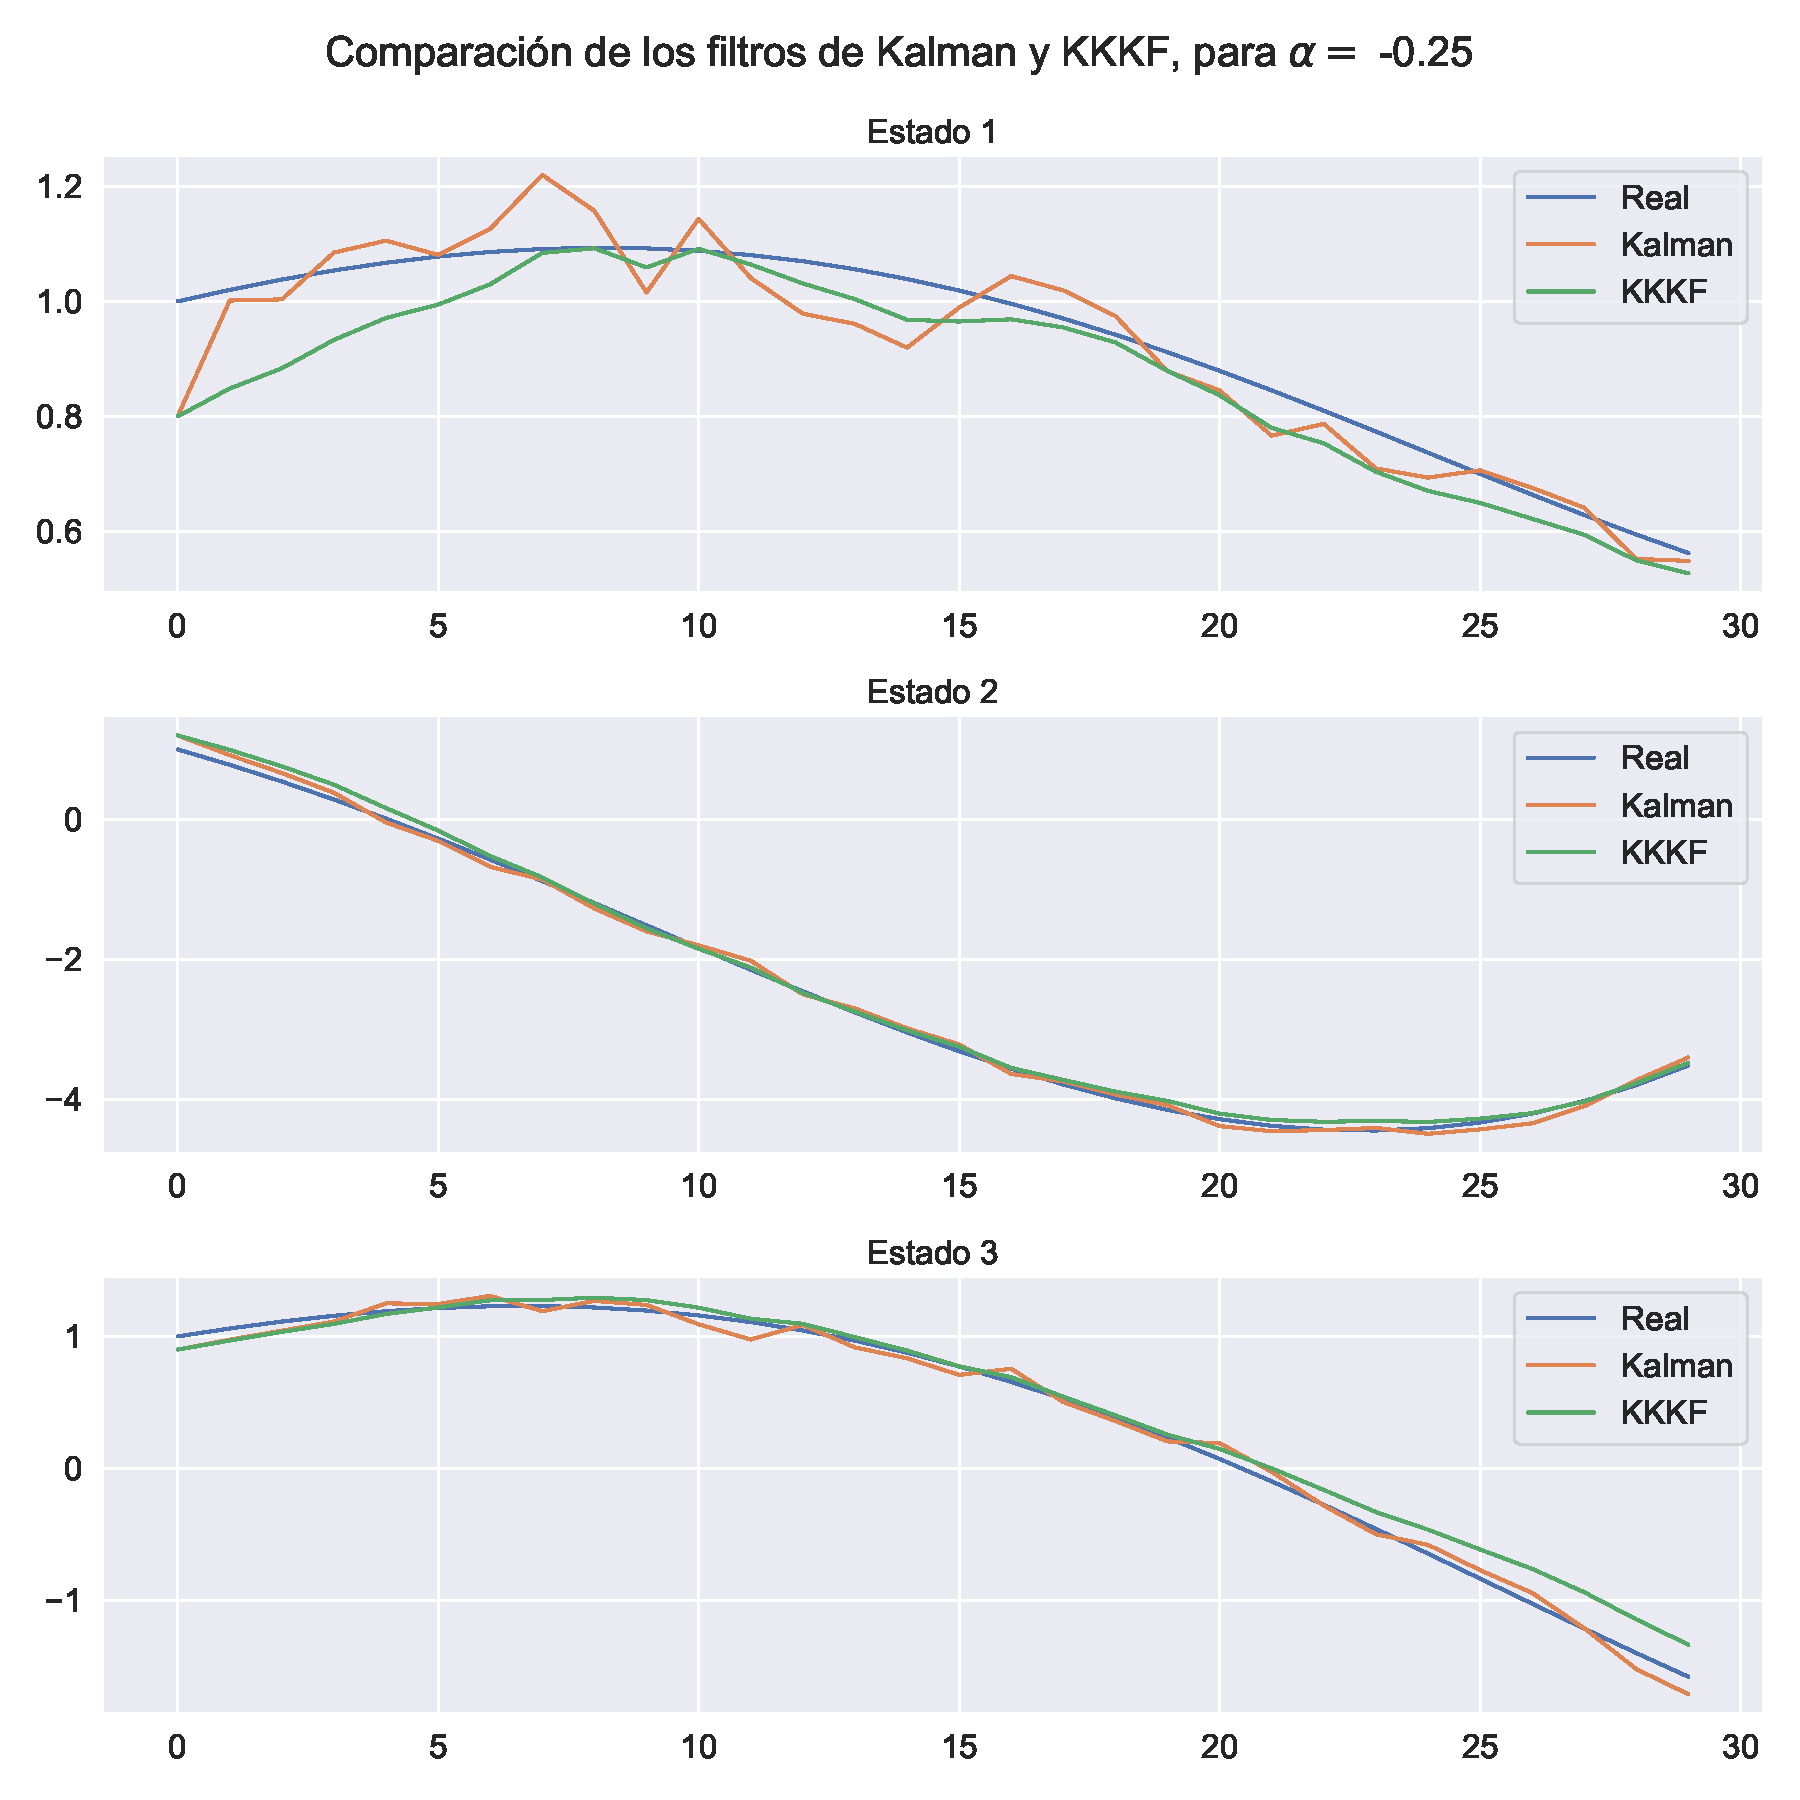
\includegraphics[width=0.75\linewidth]{img/content/chapter4/kalman_vs_kerKKF_025.pdf}
    \caption{$\alpha = -0.25$.}
    \label{fig:kalman_vs_kerKKF_025}
    \end{subfigure}
    \caption{Comparación de Kalman con kerKKF para distintos valores de $\alpha$. En azul el resultado del sistema simulado sin ruidos ni de dinámica ni observación, en naranja la solución del filtro de Kalman y en verde la de kerKKF.}
\end{figure}

\section{Comparación con otros filtros para modelos epidemiológicos}

\begin{figure}[h!]
    \centering
    \begin{subfigure}[b]{0.49\textwidth}
        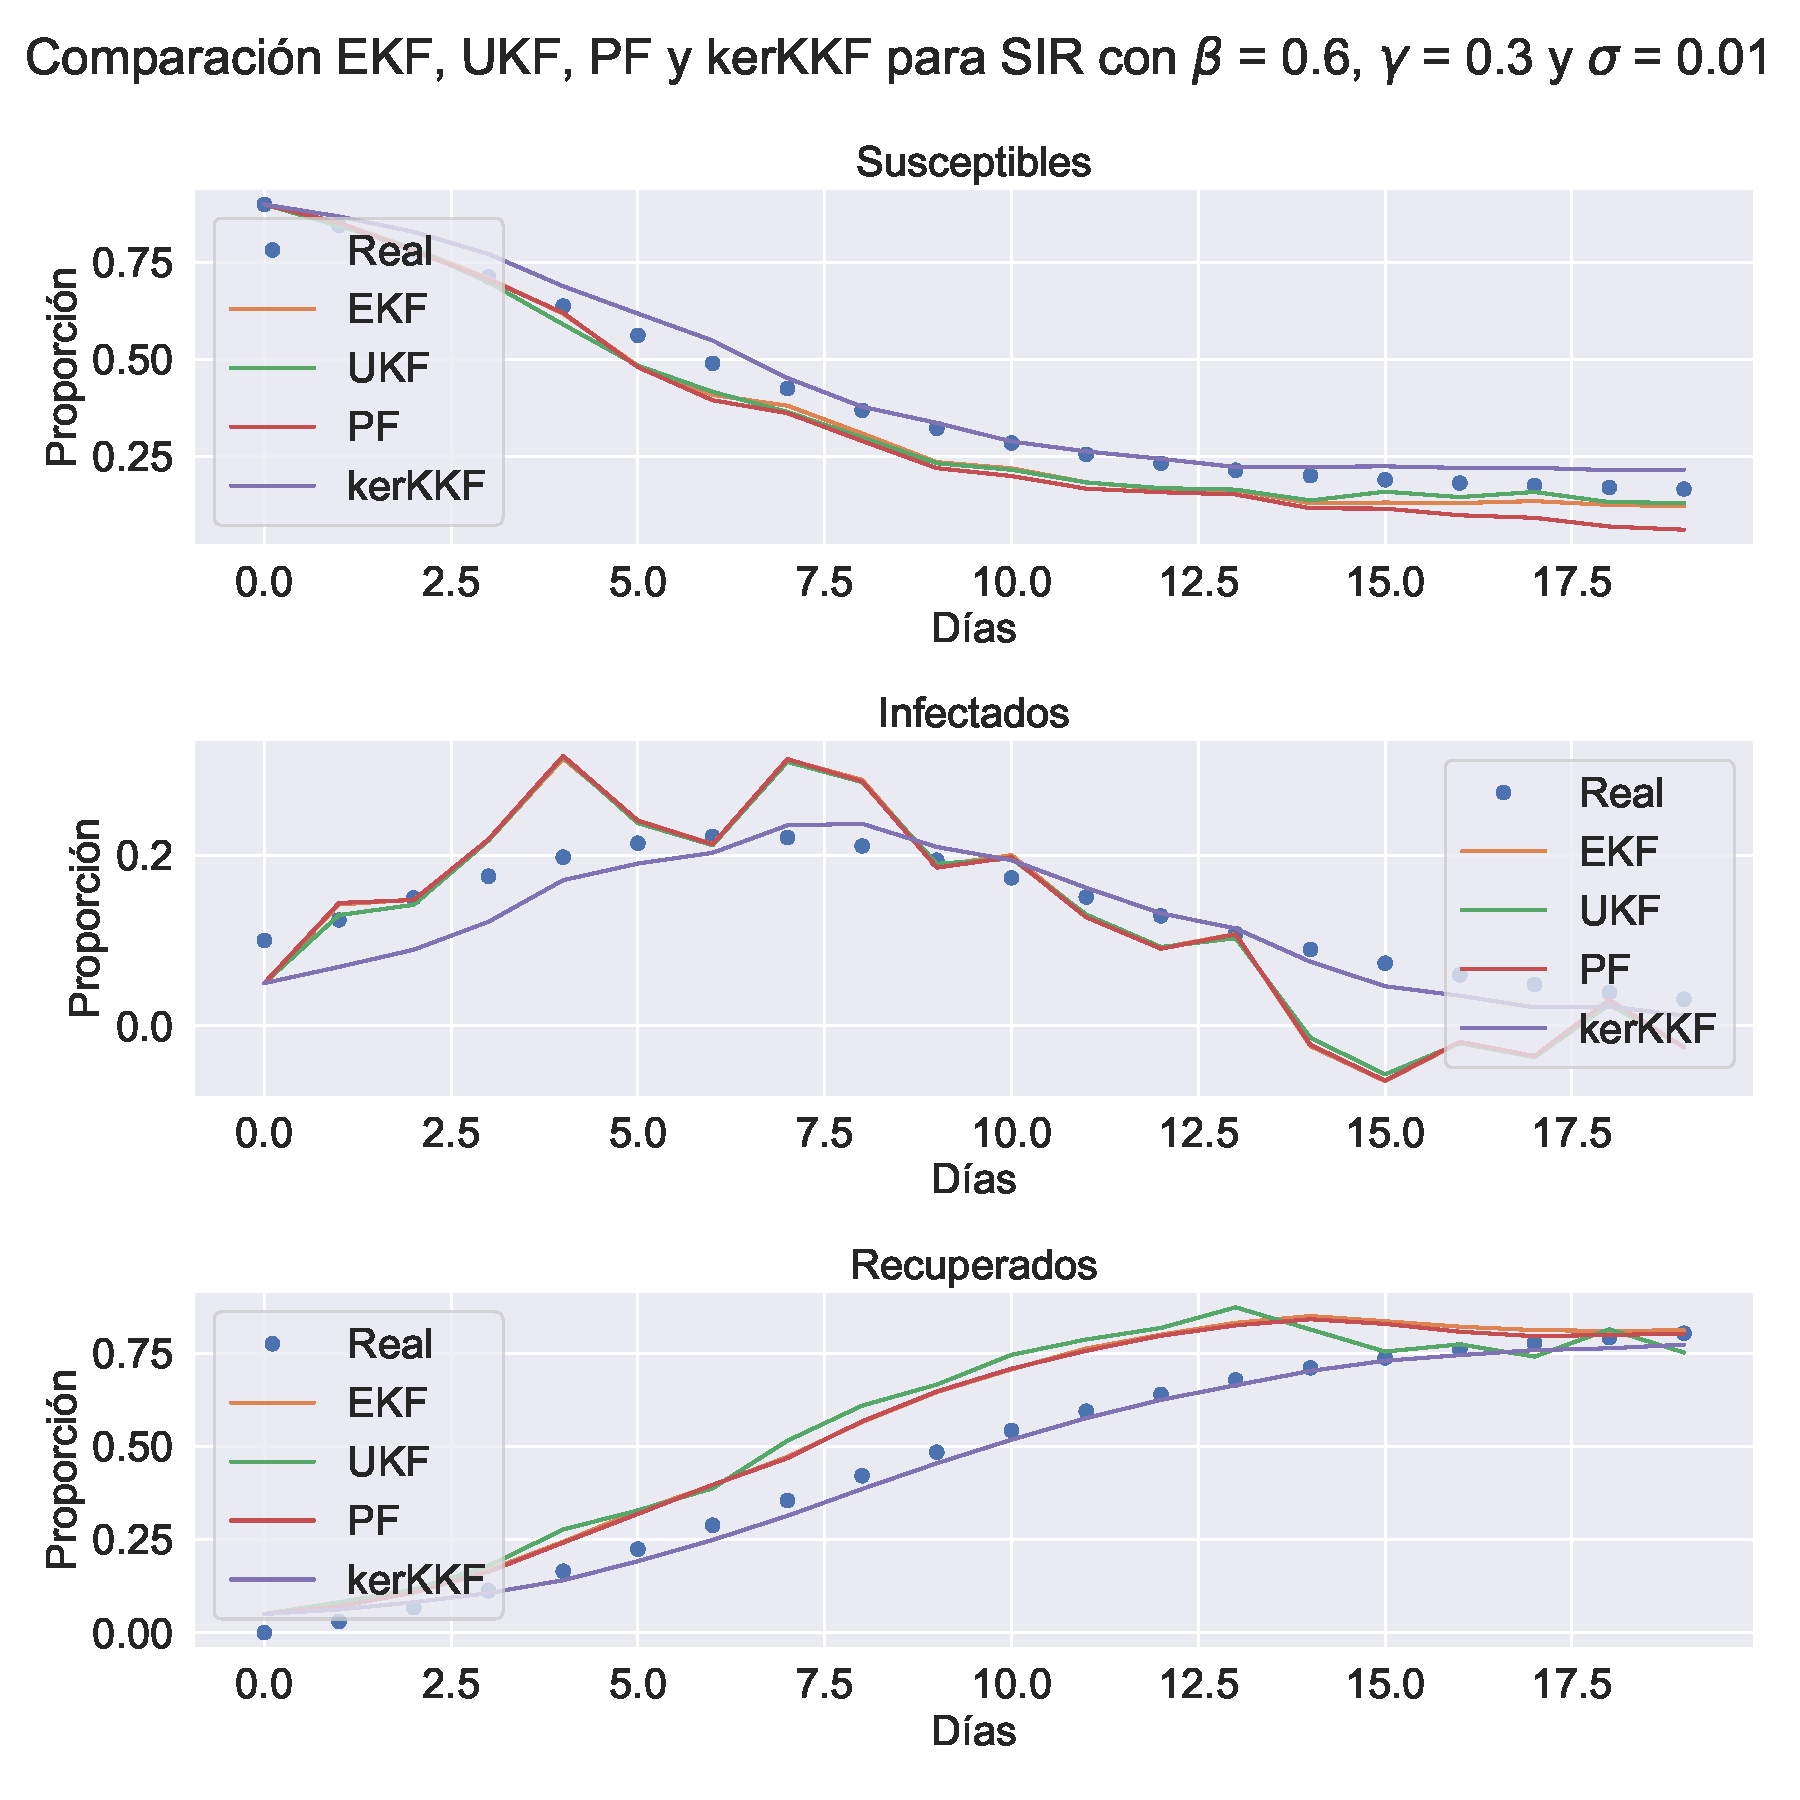
\includegraphics[width=\linewidth]{img/content/chapter4/nonlinear_filters_sir_beta_06.pdf}
    \caption{$\beta = 0.6$.}
    \label{fig:nonlinear_filters_sir_beta_06}
    \end{subfigure}
    \begin{subfigure}[b]{0.49\textwidth}
        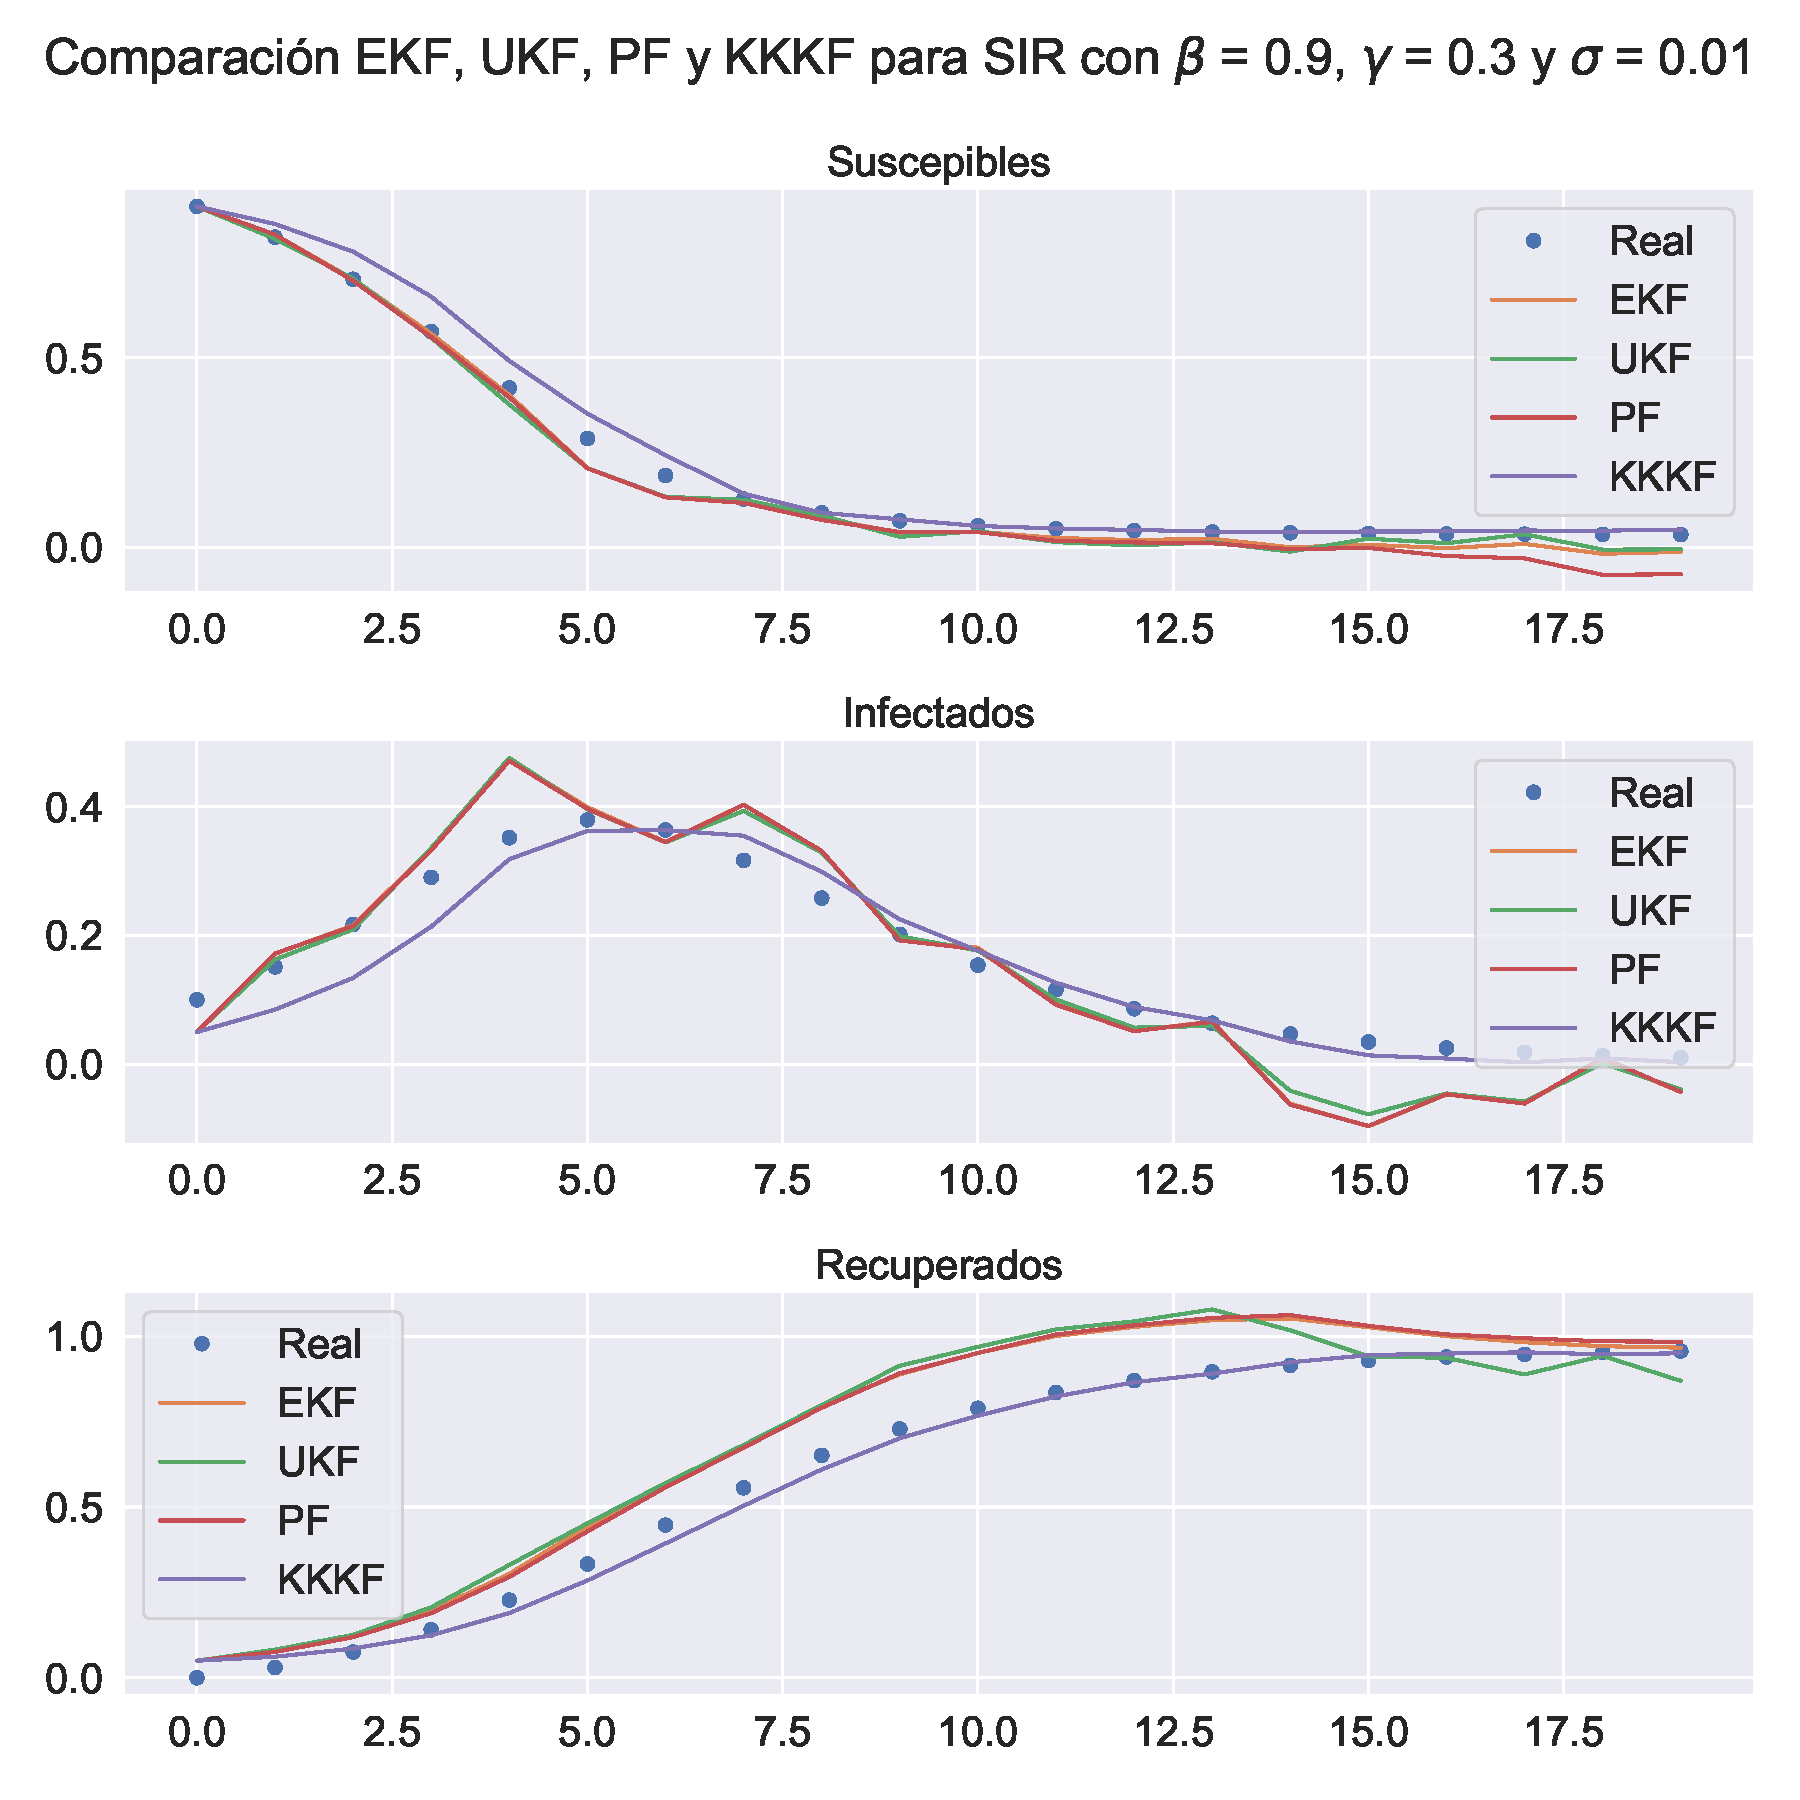
\includegraphics[width=\linewidth]{img/content/chapter4/nonlinear_filters_sir_beta_09.pdf}
    \caption{$\beta = 0.9$.}
    \label{fig:nonlinear_filters_sir_beta_09}
    \end{subfigure}
    \begin{subfigure}[b]{0.49\textwidth}
        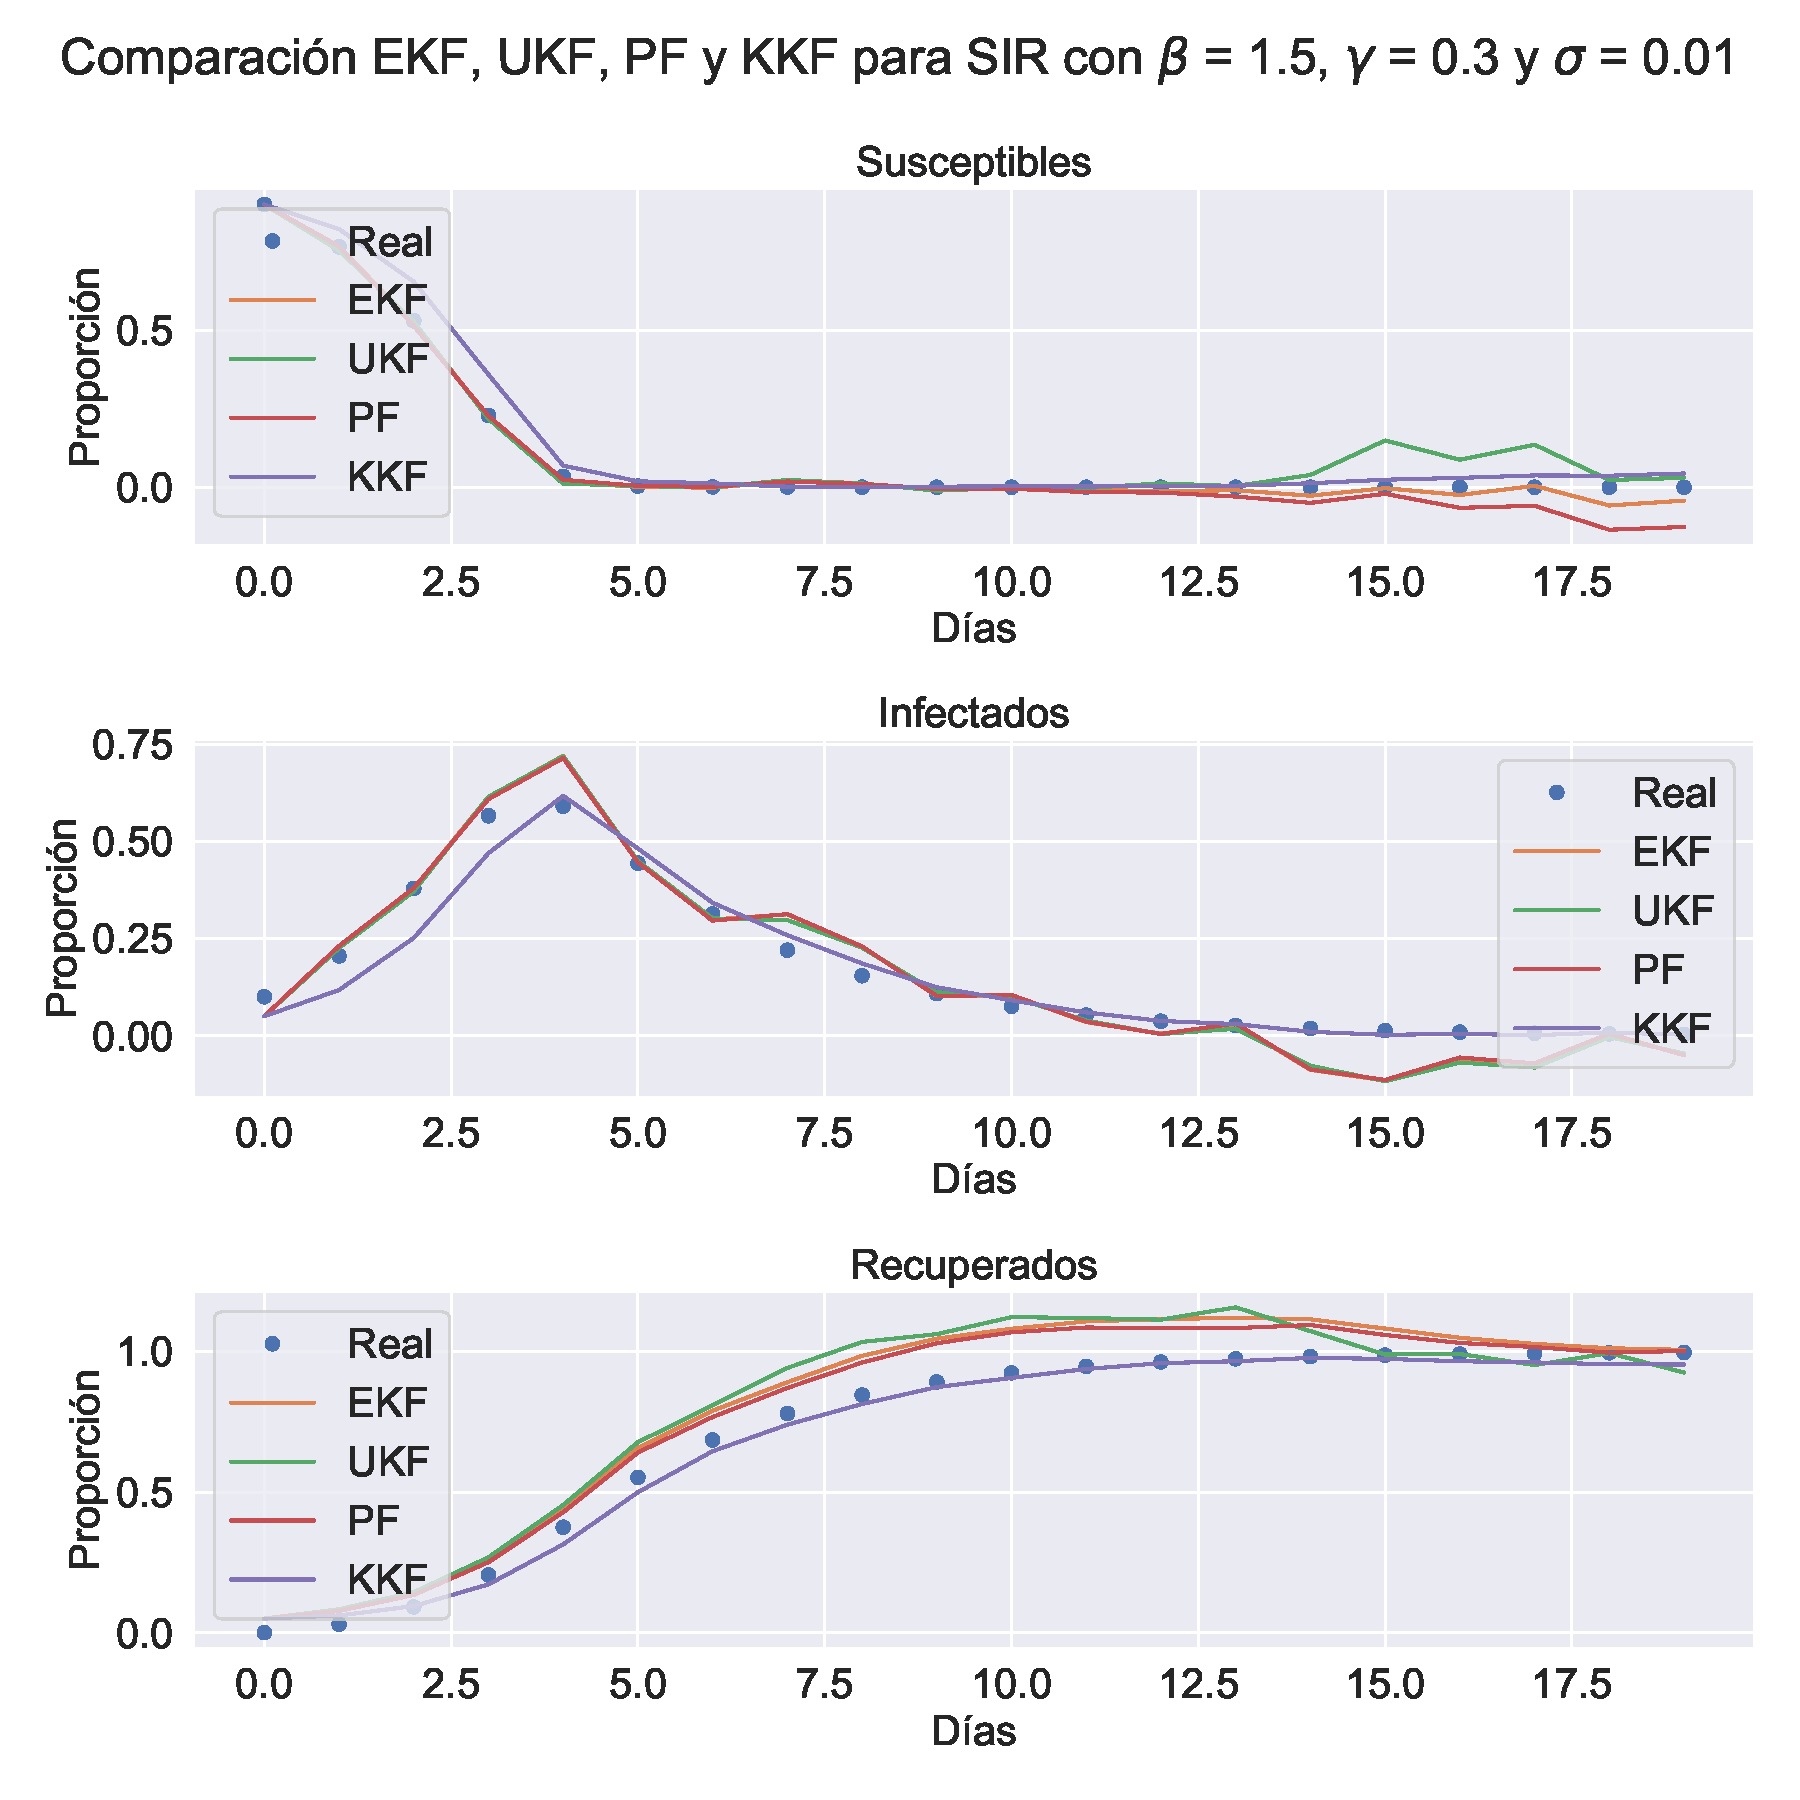
\includegraphics[width=\linewidth]{img/content/chapter4/nonlinear_filters_sir_beta_15.pdf}
    \caption{$\beta = 1.5$.}
    \label{fig:nonlinear_filters_sir_beta_15}
    \end{subfigure}
    \caption{Comparación de resultados de las trayectorias generadas por los filtros EKF (naranja), UKF (verde), PF (rojo) y kerKKF (púrpura), junto con la trayectoria real (puntos azules) sin ruidos, ni de dinámica ni de observación, esto para cada uno de los estados del modelo SIR. $\beta$ varía en cada caso para (a), (b) y (c), mientras que $\gamma = 0.3$ y $\sigma = 0.01$ fijos.}
\end{figure}

\begin{table}[h!]
    \caption{Errores para distintos valores de $\beta$, parámetro que representa la no linealidad del sistema. Esto para $\gamma = 0.3$ y $\sigma = 0.01$ fijos.}
    \begin{subtable}{\linewidth}
        \centering
    \caption{Errores para $\beta = 0.6$ y $\gamma = 0.3$}
    \begin{tabular}{|c|c|c|c|c|}
    \hline
    \textbf{Estado} & \textbf{EKF} & \textbf{UKF} & \textbf{PF} & \textbf{kerKKF} \\ \hline
    S & 0.2442 & 0.2379 & 0.3305 & 0.1629 \\ \hline
    I & 0.2904 & 0.2815 & 0.2903 & 0.1352 \\ \hline
    R & 0.4874 & 0.5503 & 0.4732 & 0.1210 \\ \hline
    \end{tabular}
    \label{tab:errores_beta_gamma_06}
    \end{subtable}
    \begin{subtable}{\linewidth}
        \centering
    \caption{Errores para $\beta = 0.9$ y $\gamma = 0.3$}
    \begin{tabular}{|c|c|c|c|c|}
    \hline
    \textbf{Estado} & \textbf{EKF} & \textbf{UKF} & \textbf{PF} & \textbf{kerKKF} \\ \hline
    S & 0.1486 & 0.1533 & 0.2195 & 0.1672 \\ \hline
    I & 0.2808 & 0.2590 & 0.2798 & 0.1628 \\ \hline
    R & 0.4866 & 0.5246 & 0.4907 & 0.1300 \\ \hline
    \end{tabular}
    \label{tab:errores_beta_gamma_09}
    \end{subtable}
    \begin{subtable}{\linewidth}
        \centering
    \caption{Errores para $\beta = 1.5$ y $\gamma = 0.3$}
    \begin{tabular}{|c|c|c|c|c|}
    \hline
    \textbf{Estado} & \textbf{EKF} & \textbf{UKF} & \textbf{PF} & \textbf{kerKKF} \\ \hline
    S & 0.0885 & 0.2296 & 0.2292 & 0.1906 \\ \hline
    I & 0.2834 & 0.2788 & 0.2816 & 0.1934 \\ \hline
    R & 0.4671 & 0.5295 & 0.4042 & 0.1435 \\ \hline
    \end{tabular}
    \label{tab:errores_beta_gamma_15}
    \end{subtable}
\end{table}

\begin{figure}[h!]
    \centering
    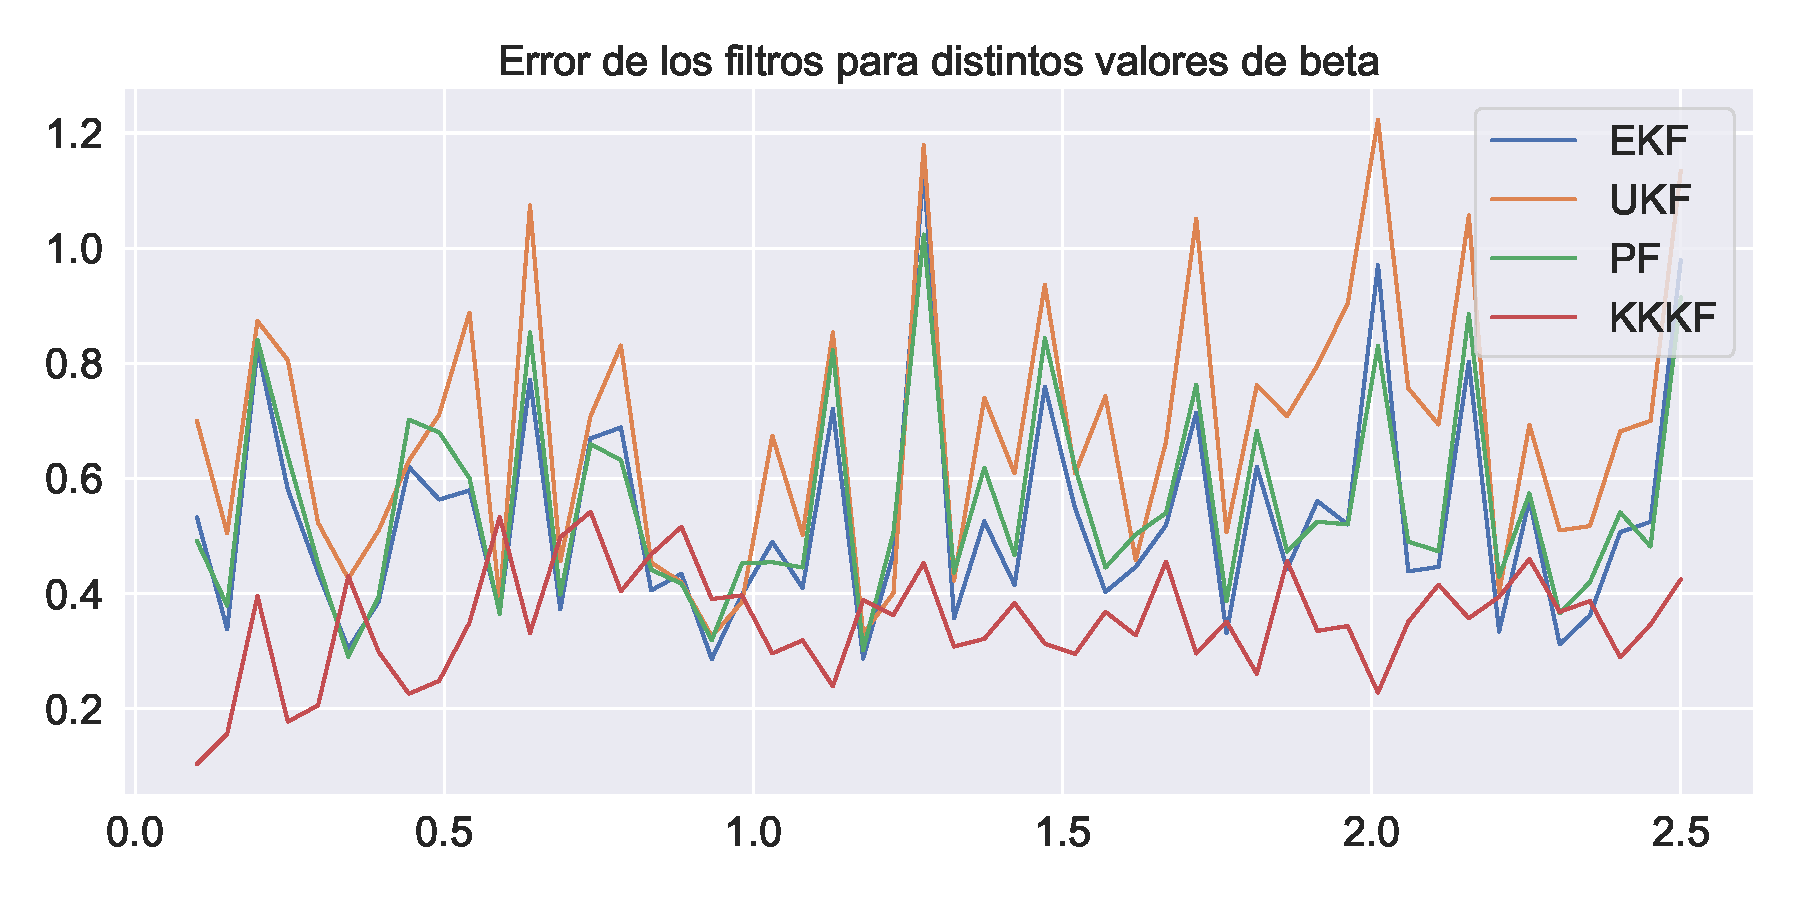
\includegraphics[width=0.9\linewidth]{img/content/chapter4/nonlinear_filters_sir_error_beta.pdf}
    \caption{Error en norma de EKF (azul), UKF (naranja), PF (verde) y kerKKF (rojo) para distintos valores de $\beta$ entre $0.1$ y $2.5$. Eje y en escala logarítmica.}
    \label{fig:nonlinear_filters_sir_error_beta}
\end{figure}

\newpage

\section{Comparación con métodos de Markov Chain Monte Carlo}


\begin{figure}[h!]
    \centering
    \begin{subfigure}[b]{0.49\textwidth}
    \centering
         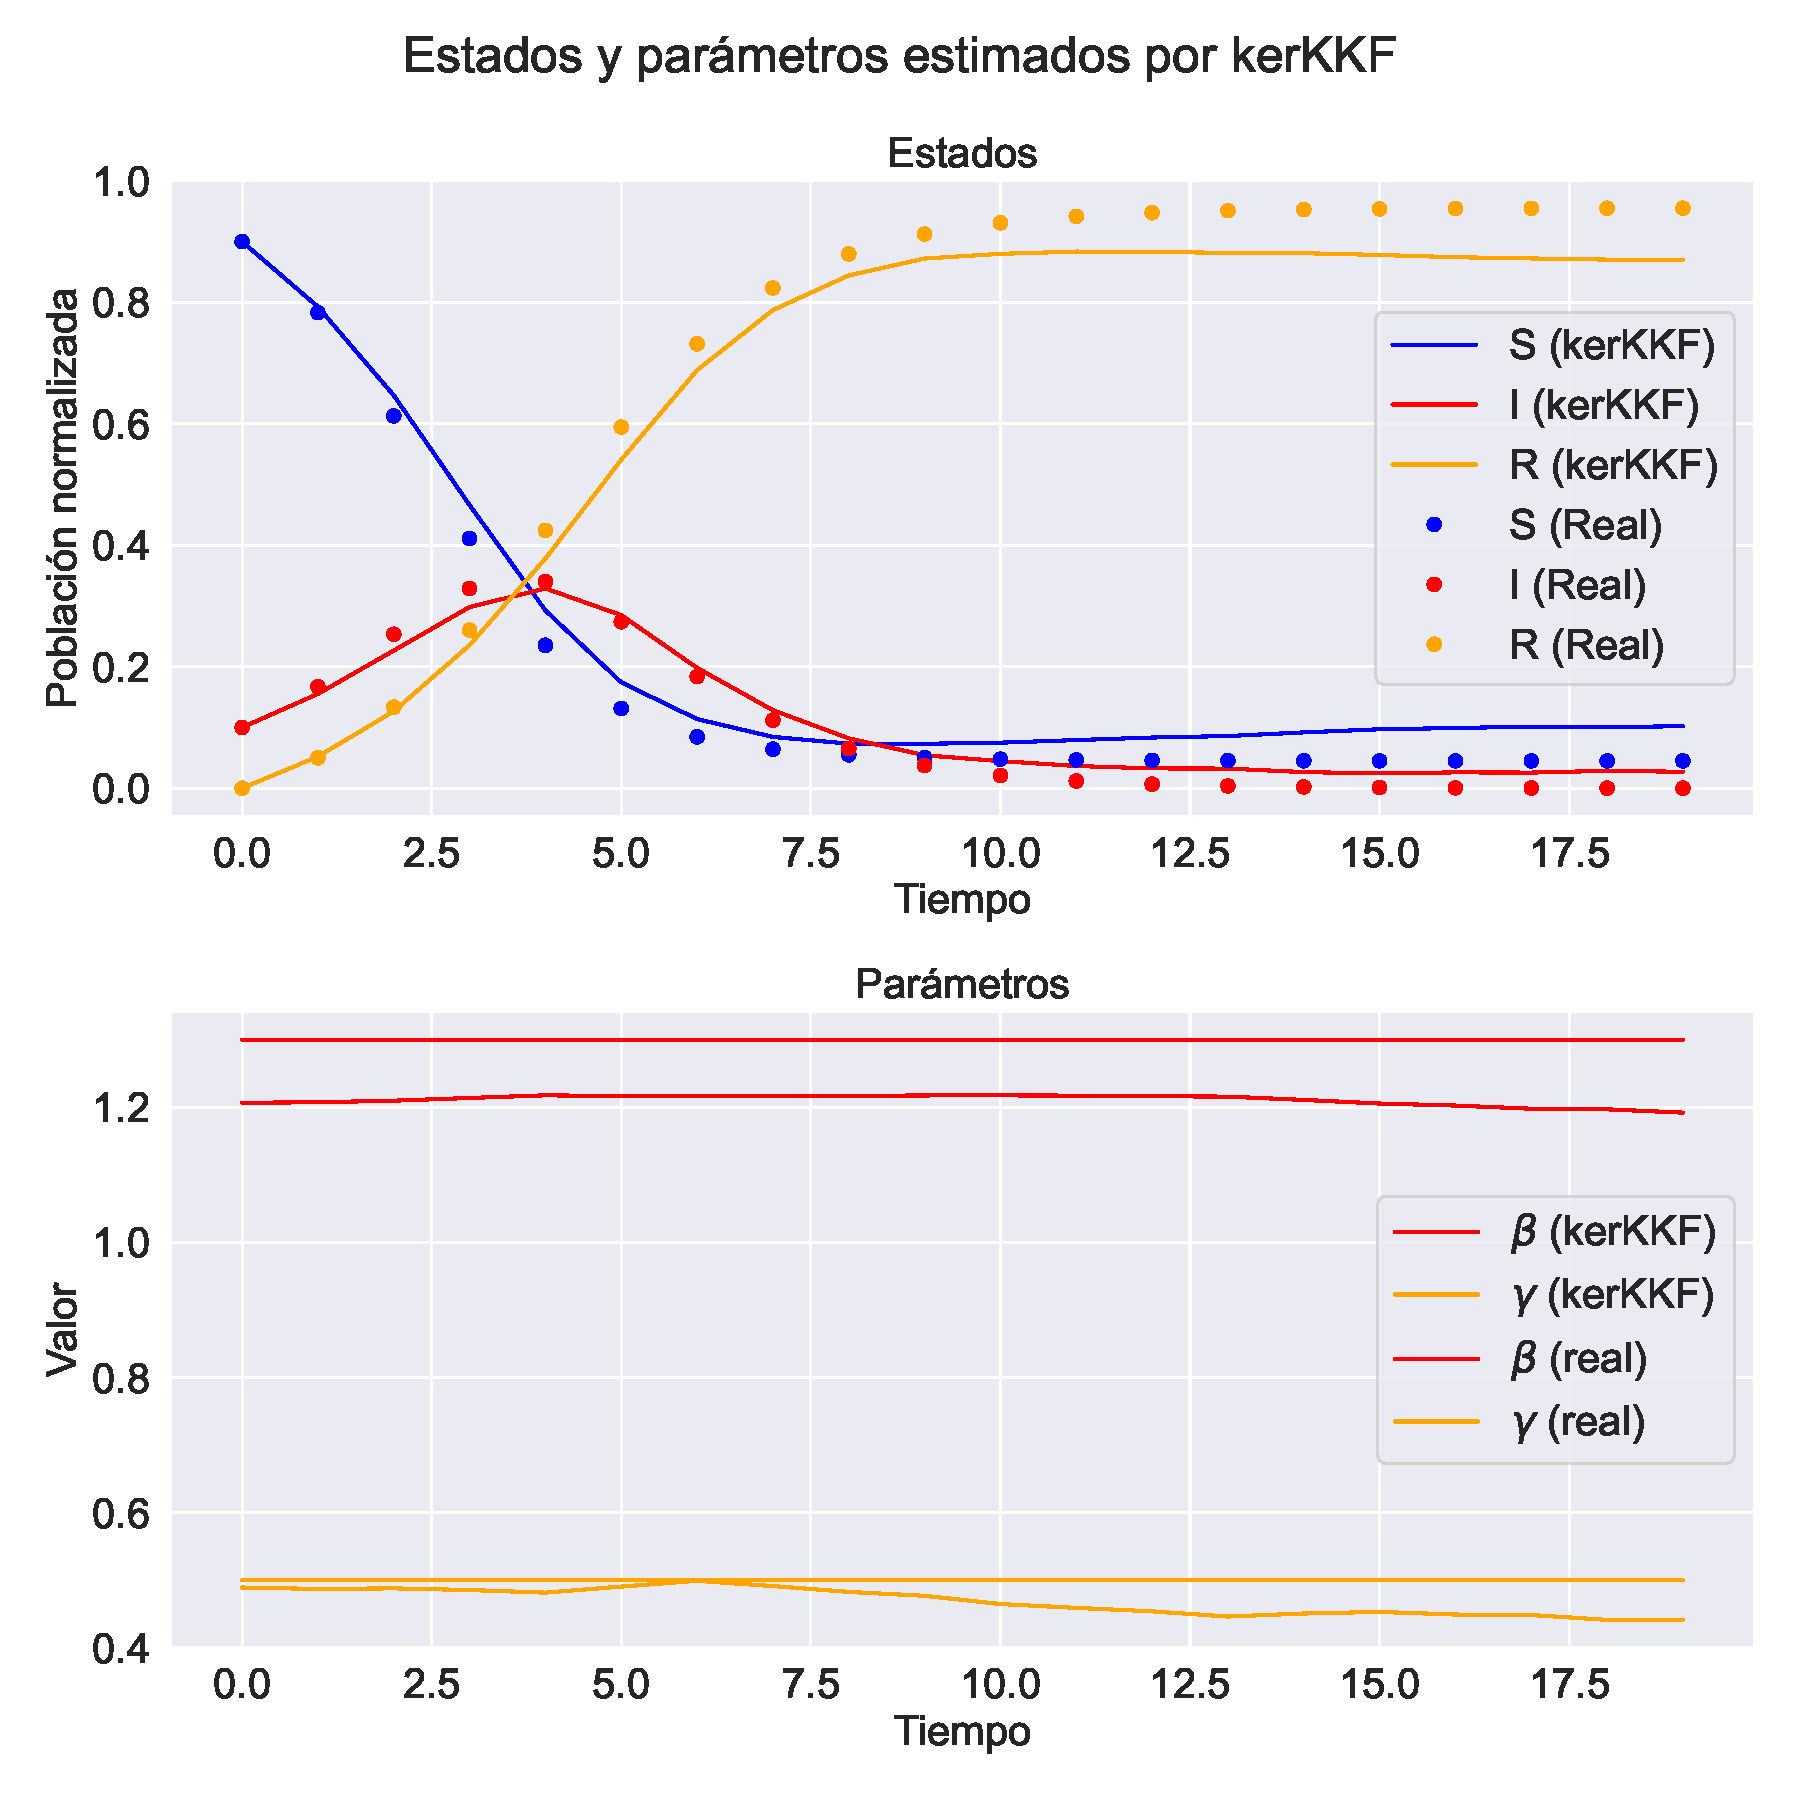
\includegraphics[width=0.8\linewidth]{img/content/chapter4/nonlinear_filters_sir_params.pdf}
    \caption{}
    \end{subfigure}
   \begin{subfigure}[b]{0.49\textwidth}
   \centering
       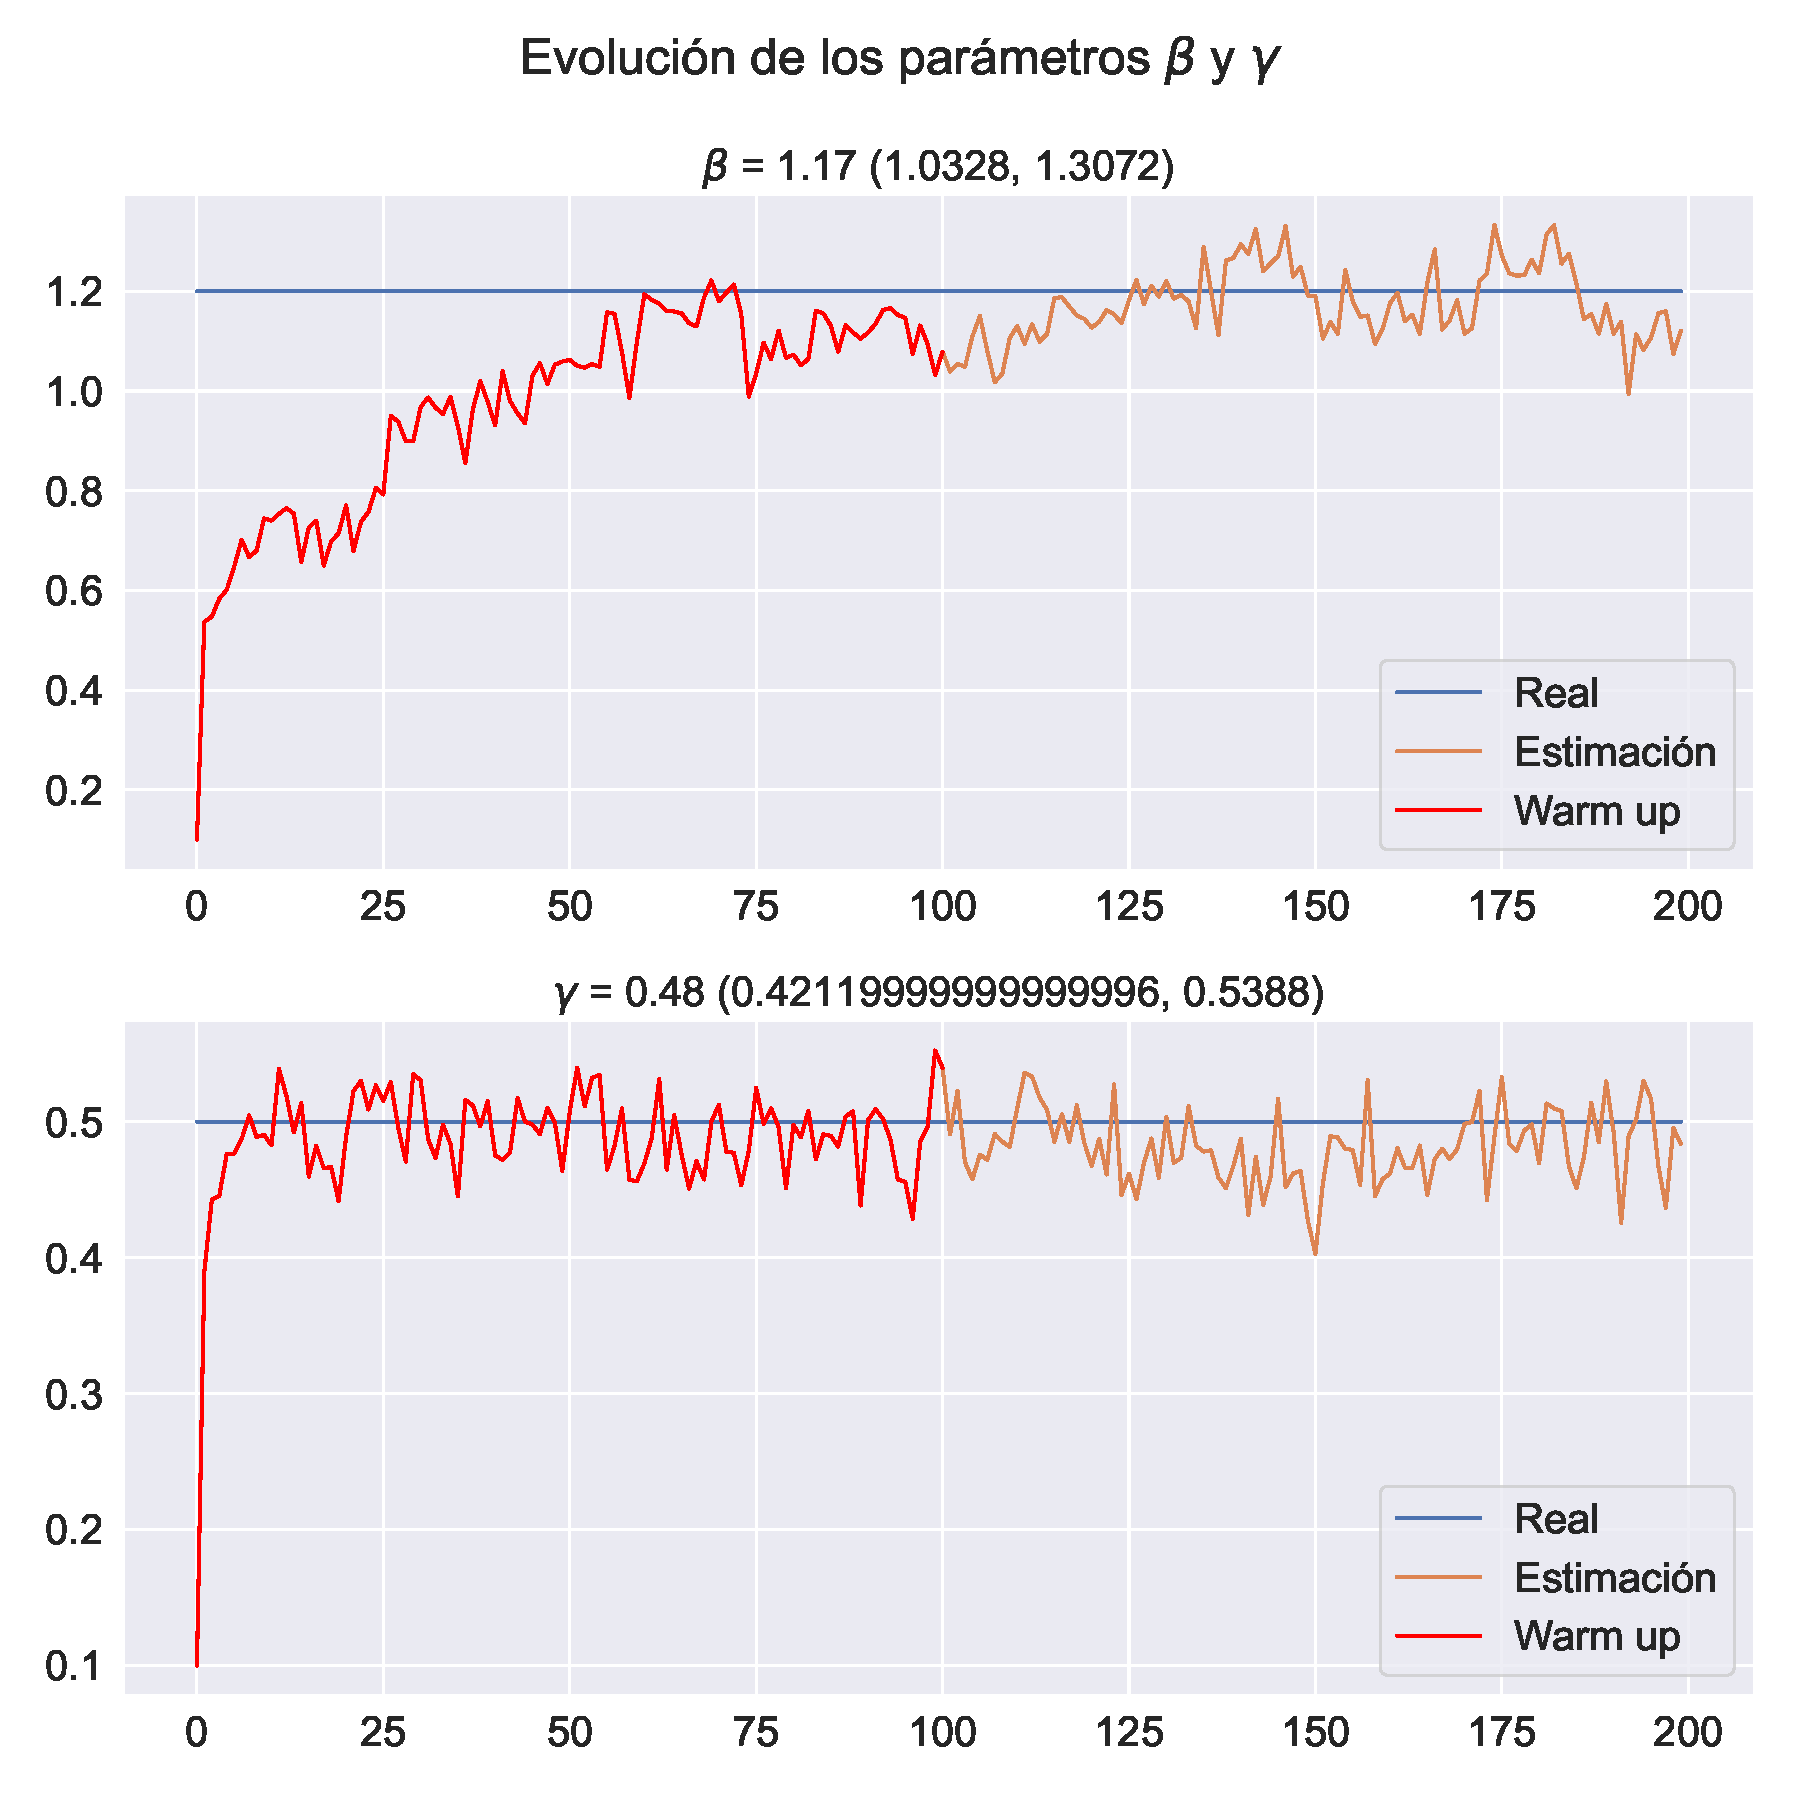
\includegraphics[width=0.8\linewidth]{img/content/chapter4/nonlinear_filters_sir_params_evolution.pdf}
       \caption{}
   \end{subfigure}
    \caption{Resultado para modelo SIR \eqref{eq:SIR}. \\
    (a) Resultado de kerKKF para estimación de parámetros, primera cadena. \\
    (b) Evolución de la estimación de los parámetros a través de las iteraciones del algoritmo de estimación, primera cadena. De color rojo, el régimen de \textit{warm up}, mientras que en naranja se encuentran que sí serán consideradas para la estimación. En azul se encuentra el valor real del parámetro.}
    \label{fig:param_estim_SIR}
\end{figure}

\begin{figure}[h!]
    \centering
    \begin{subfigure}[b]{0.8\textwidth}
        \centering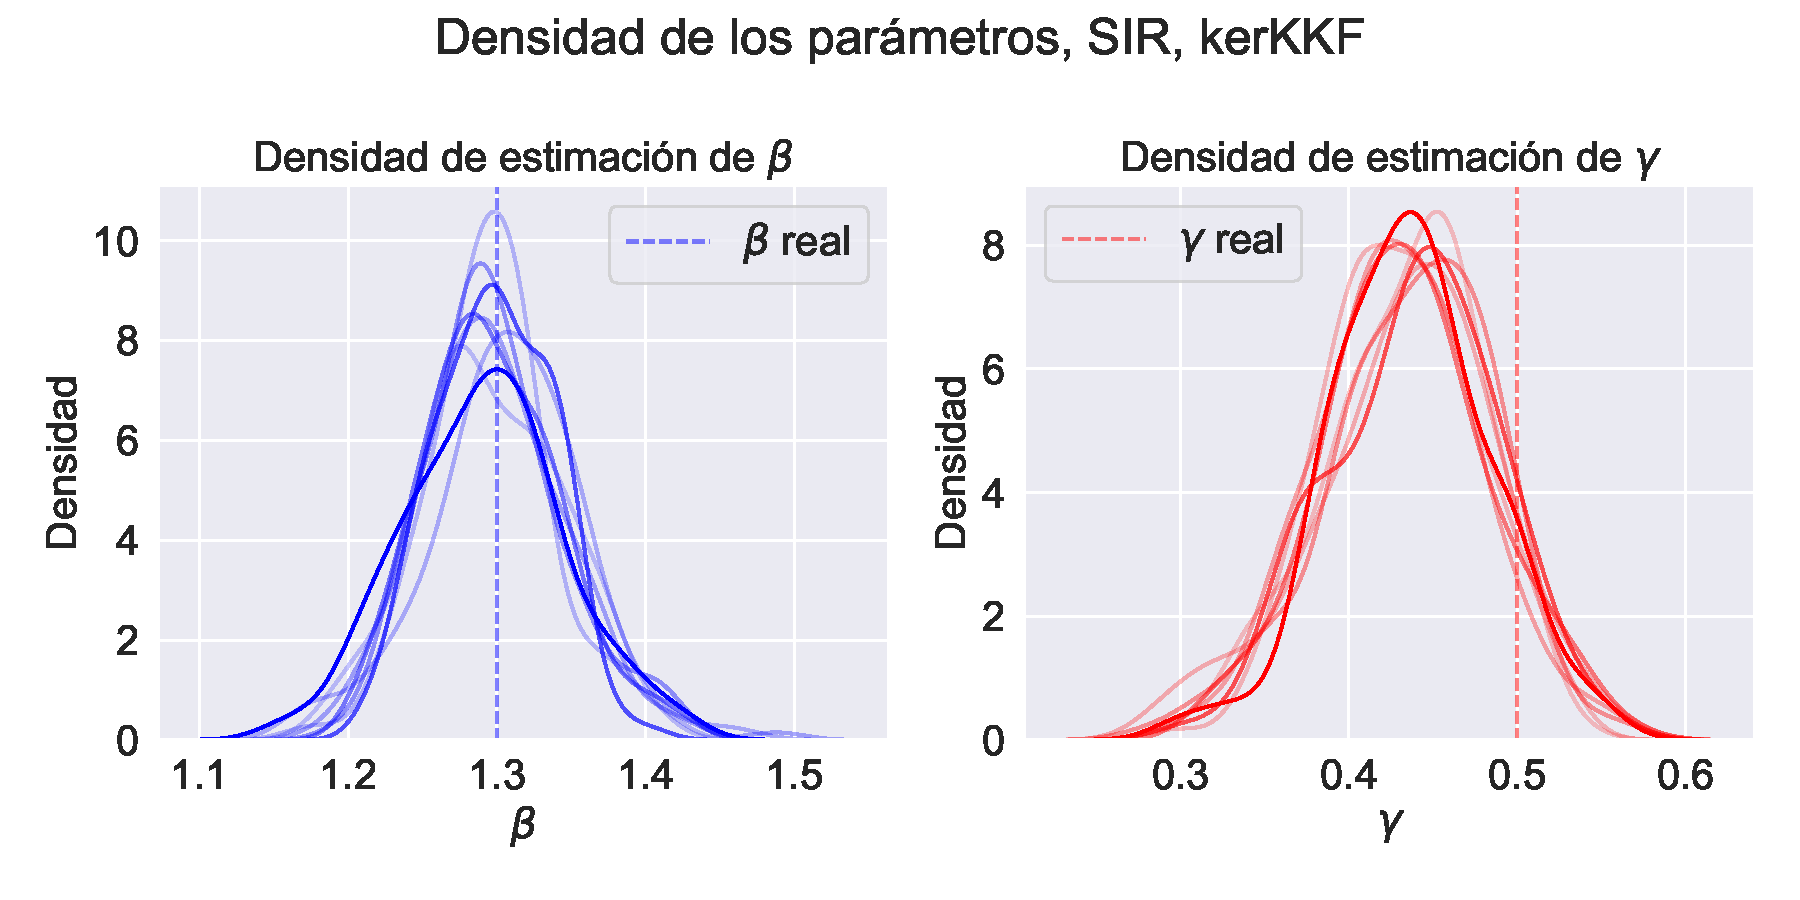
\includegraphics[width=0.8\linewidth]{img/content/chapter4/nonlinear_filters_sir_params_density.pdf}
    \caption{Densidades de las 8 cadenas.}
    \label{fig:nonlinear_filters_sir_params_density}
    \end{subfigure}
        
    \begin{subfigure}[b]{0.8\textwidth}
        \centering 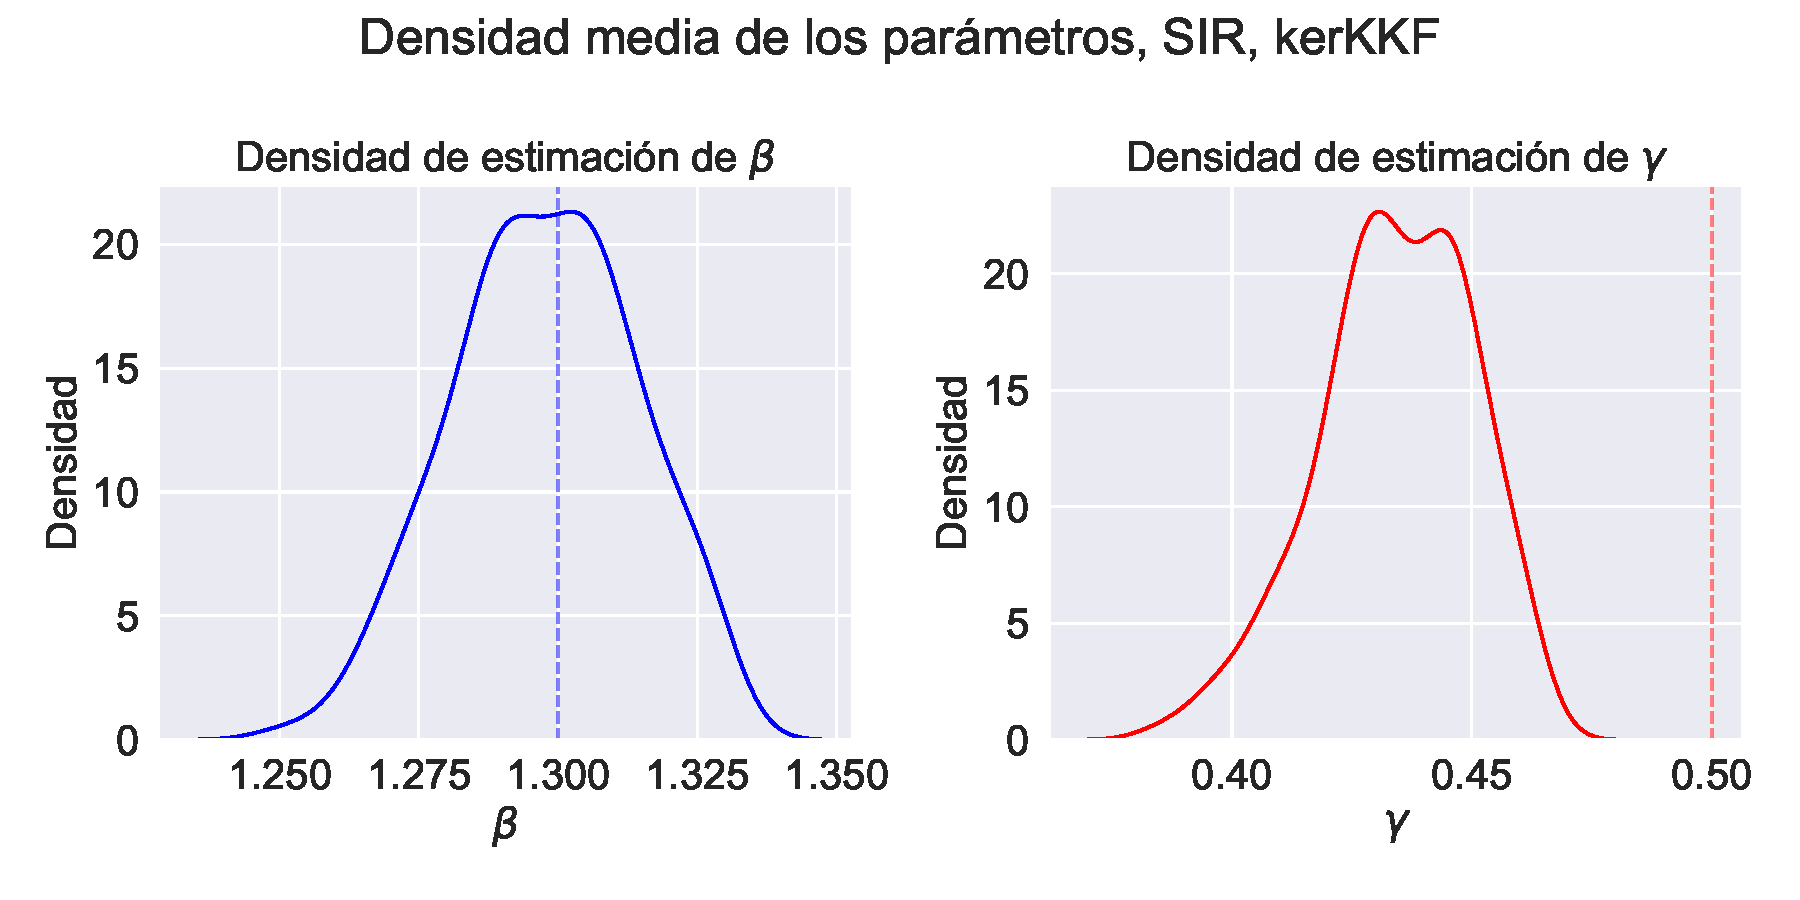
\includegraphics[width=0.8\linewidth]{img/content/chapter4/nonlinear_filters_sir_params_density_mean.pdf}
    \caption{Densidad promedio entre las 8 cadenas.}
    \label{fig:nonlinear_filters_sir_params_density_mean}
    \end{subfigure}
    \caption{Densidades de estimación para los parámetros del modelo SIR.}
\end{figure}

\begin{figure}[h!]
    \centering
    \begin{subfigure}[b]{0.49\textwidth}
         \centering
         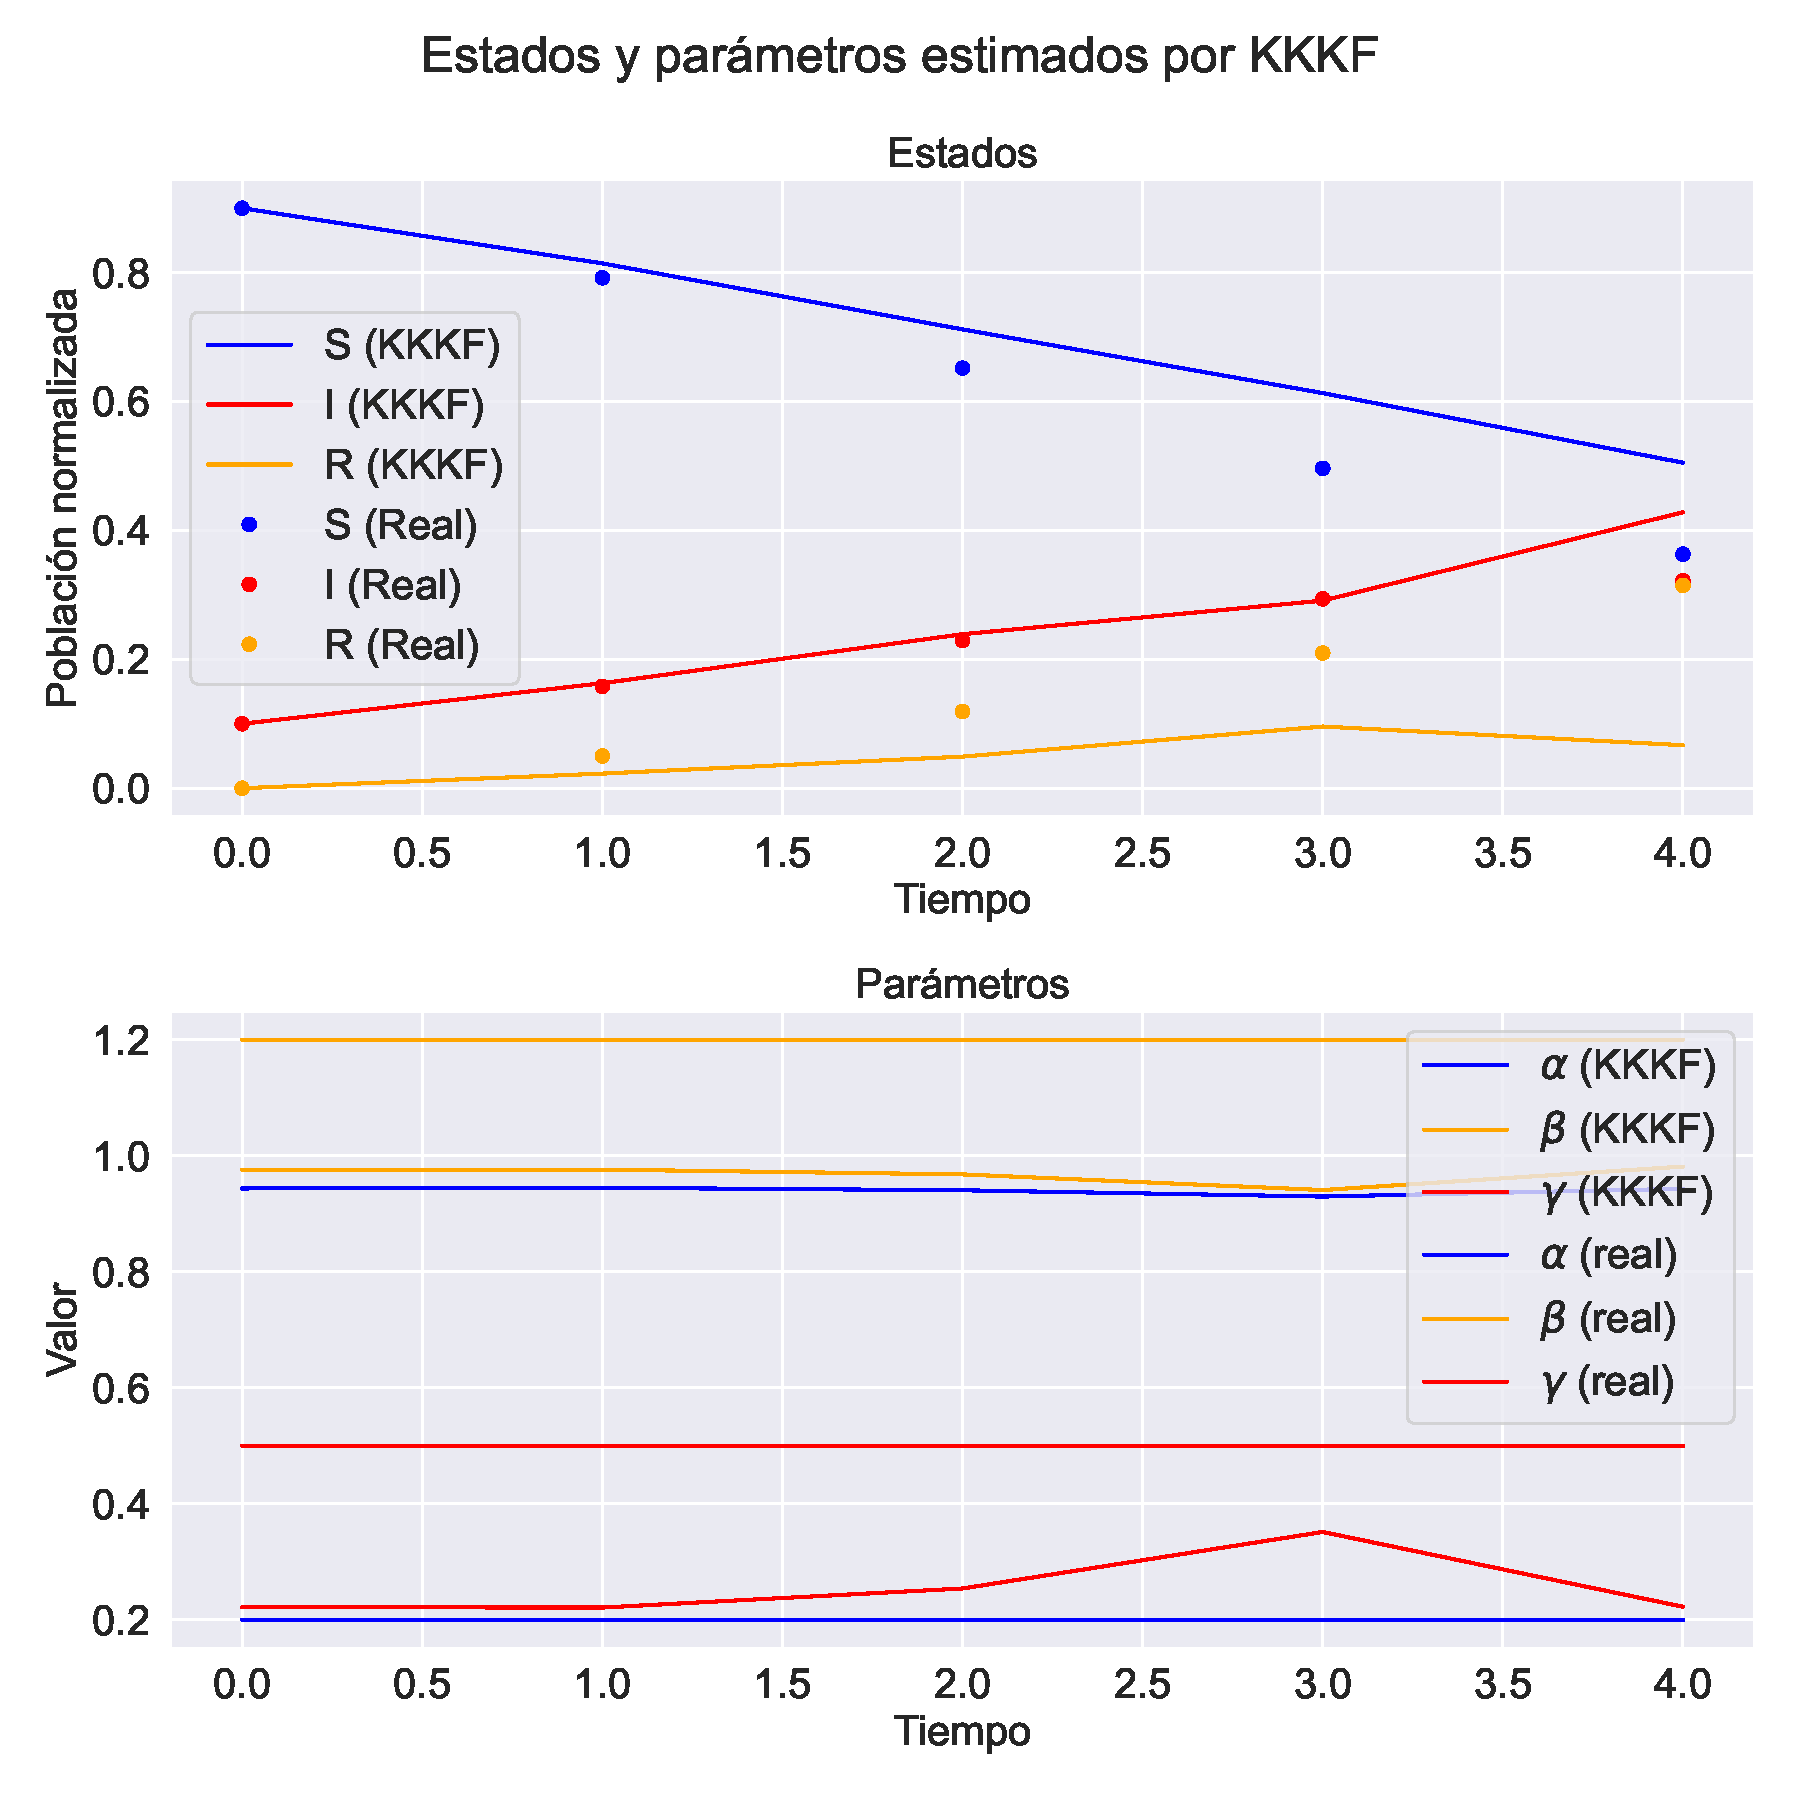
\includegraphics[height=0.9\linewidth]{img/content/chapter4/nonlinear_filters_sir_rec_params.pdf}
         \caption{}
         \label{fig:nonlinear_filters_sir_rec_params}
    \end{subfigure}
    \begin{subfigure}[b]{0.49\textwidth}
         \centering 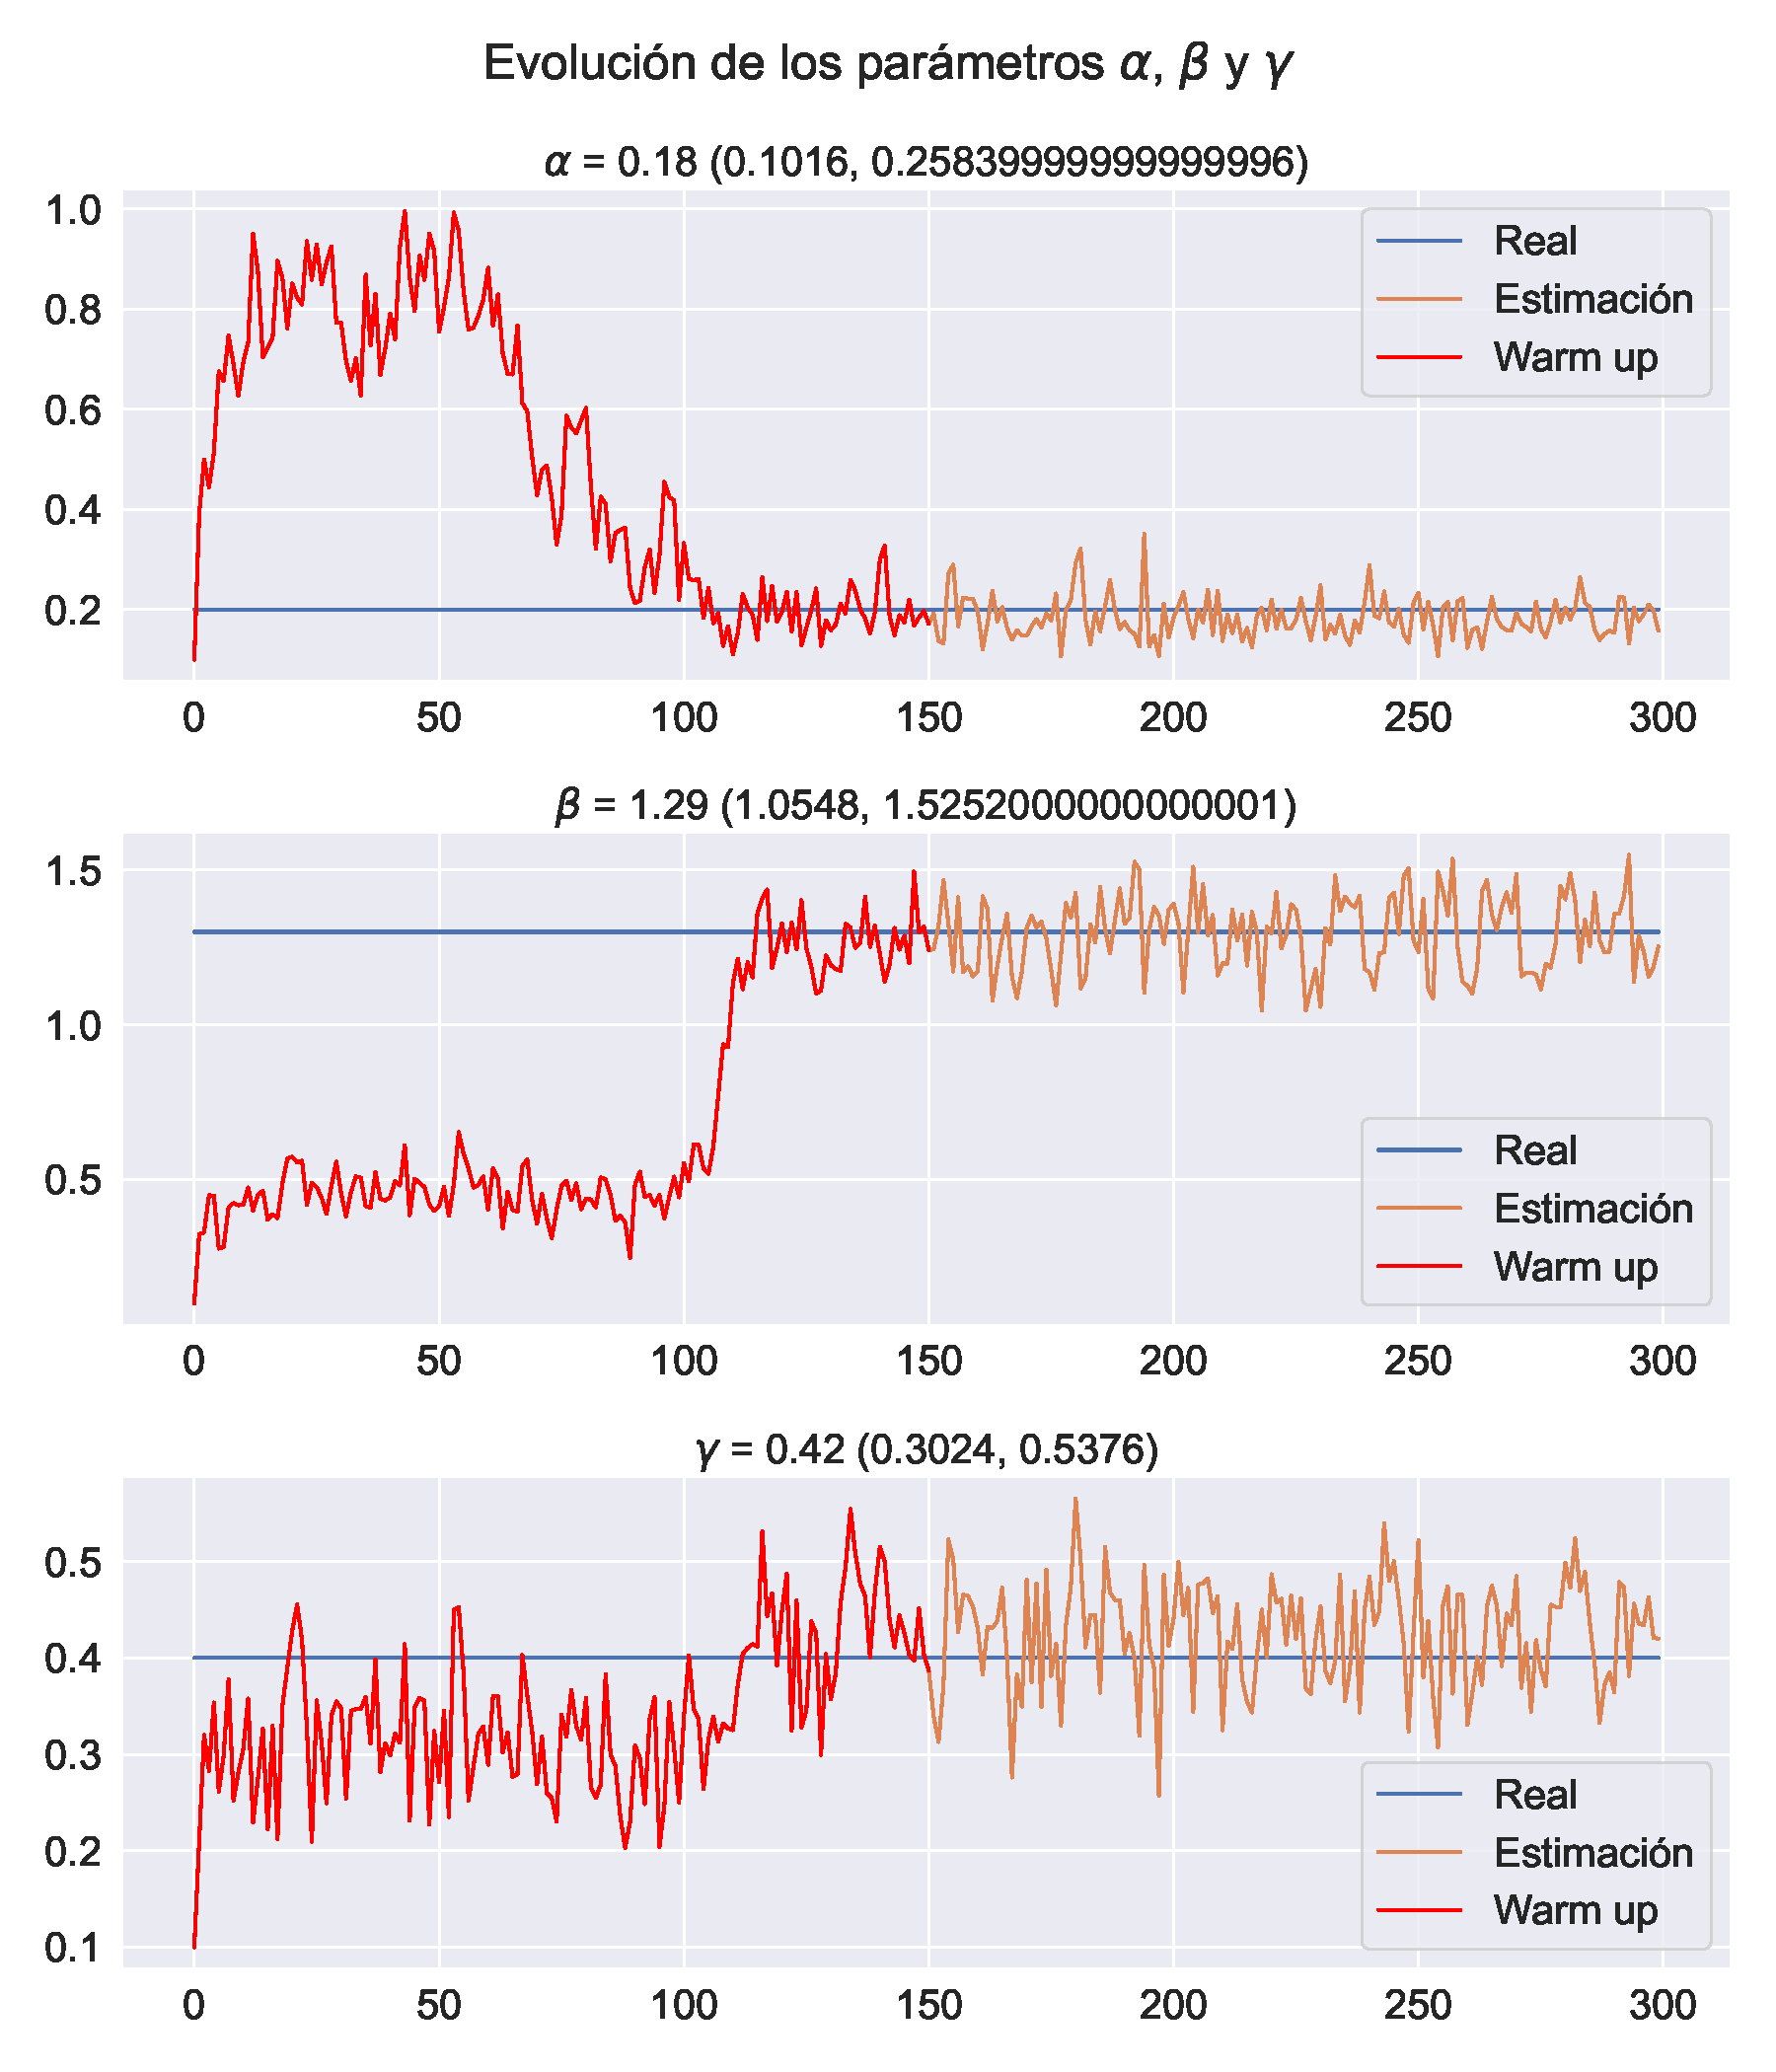
\includegraphics[height=0.9\linewidth]{img/content/chapter4/nonlinear_filters_sir_rec_params_evolution.pdf}
         \caption{}
         \label{fig:nonlinear_filters_sir_rec_params_evolution}
    \end{subfigure}
    \caption{Resultado para modelo SIR con pérdida de inmunidad \eqref{eq:SIR_rec}. \\
    (a) Resultado de kerKKF para estimación de parámetros, primera cadena. \\
    (b) Evolución de la estimación de los parámetros a través de las iteraciones del algoritmo de estimación, primera cadena. De color rojo, el régimen de \textit{warm up}, mientras que en naranja se encuentran que sí serán consideradas para la estimación. En azul se encuentra el valor real del parámetro.}
    \label{fig:SIR_inmun}
\end{figure}

\begin{figure}[h]
    \centering
    \begin{subfigure}[b]{0.8\textwidth}
        \centering 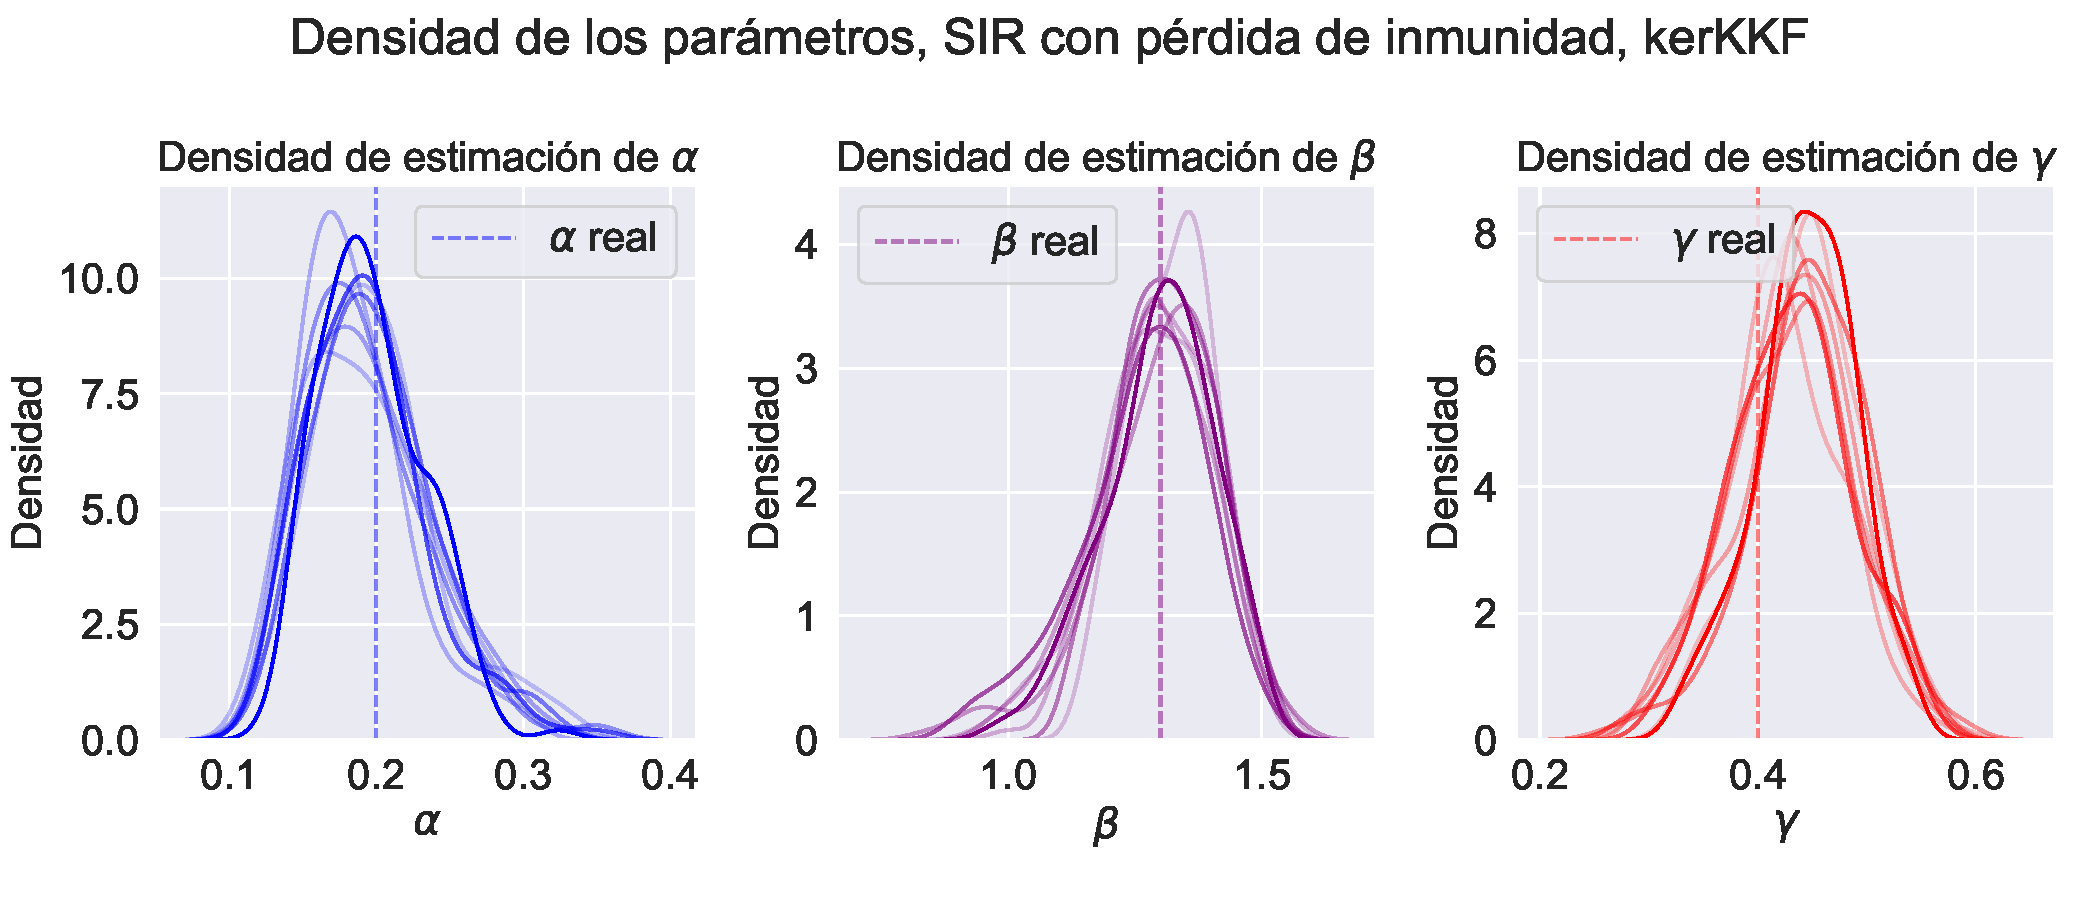
\includegraphics[width=0.8\linewidth]{img/content/chapter4/nonlinear_filters_sir_rec_params_density.pdf}
    \caption{Densidades de las 8 cadenas.}
    \label{fig:nonlinear_filters_sir_rec_params_density}
    \end{subfigure}
    \begin{subfigure}[b]{0.8\textwidth}
        \centering 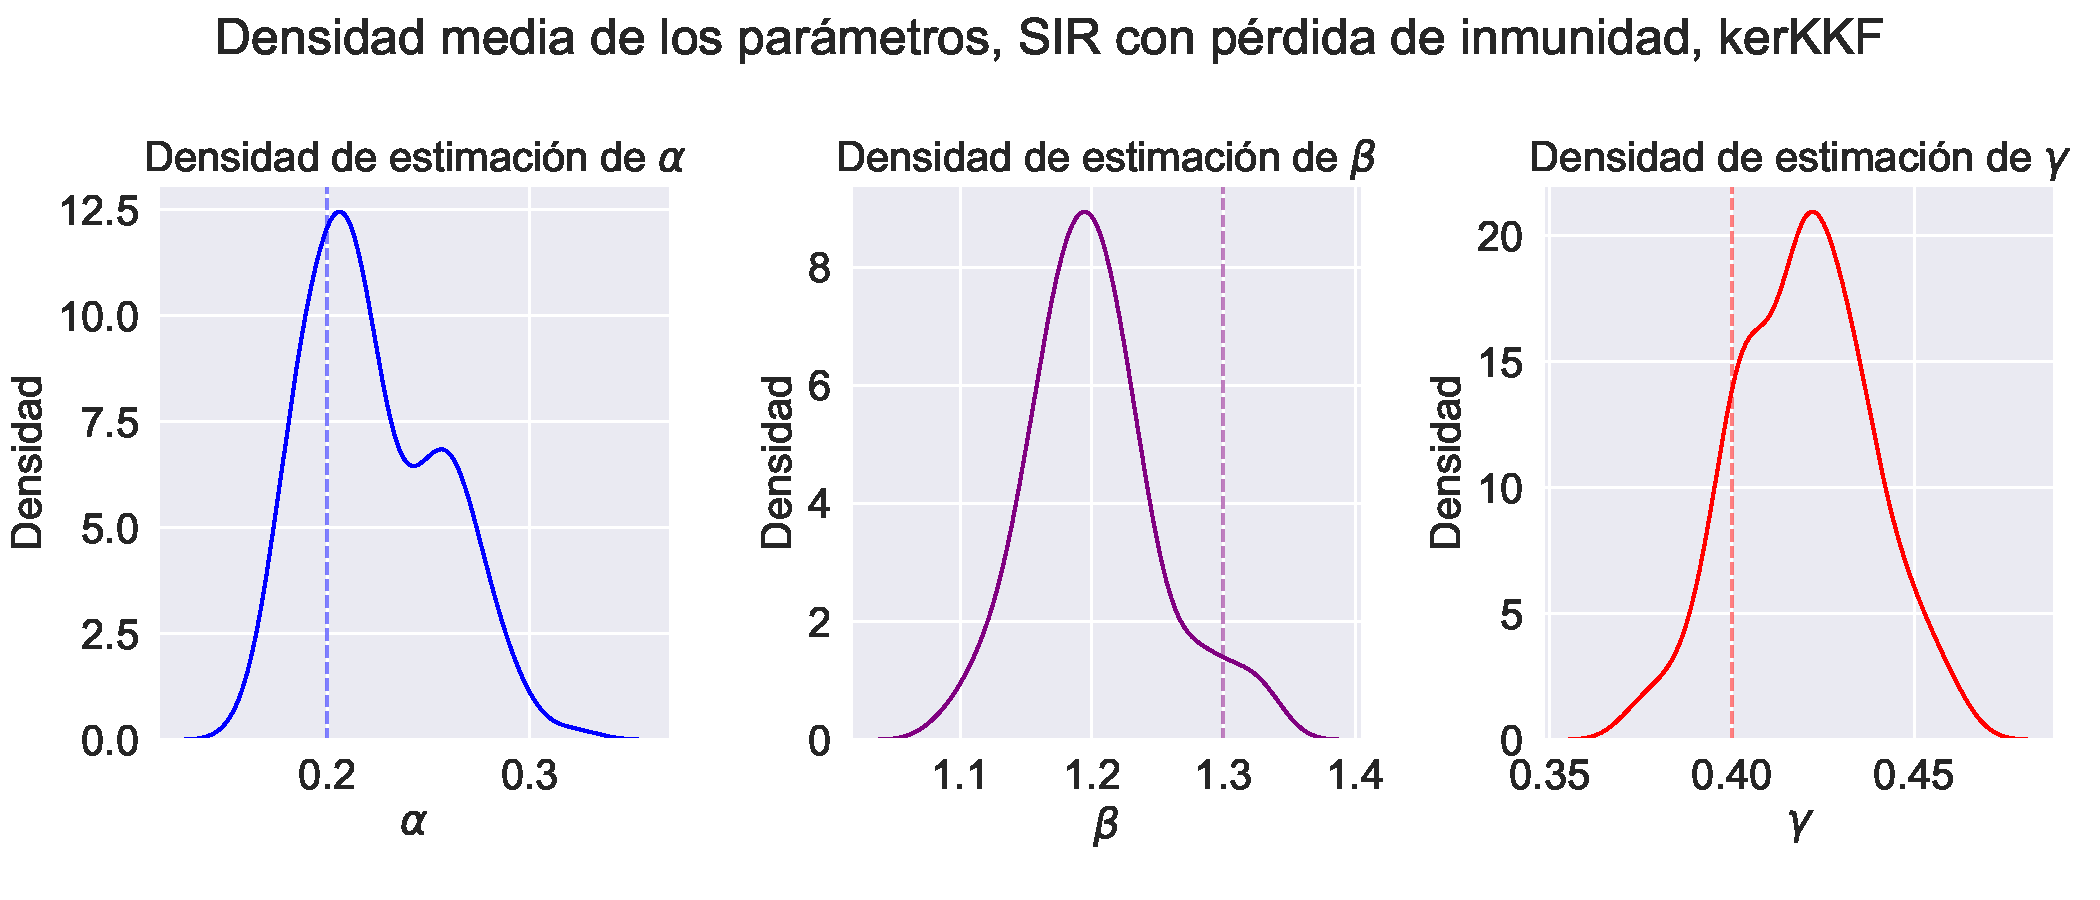
\includegraphics[width=0.8\linewidth]{img/content/chapter4/nonlinear_filters_sir_rec_params_density_mean.pdf}
    \caption{Densidad promedio entre las 8 cadenas.}
    \label{fig:nonlinear_filters_sir_rec_params_density_mean}
    \end{subfigure}
    \caption{Densidades de estimación para los parámetros del modelo SIR con pérdida de inmunidad.}
\end{figure}

\begin{figure}[h]
    \centering
    \begin{subfigure}[b]{0.49\textwidth}
         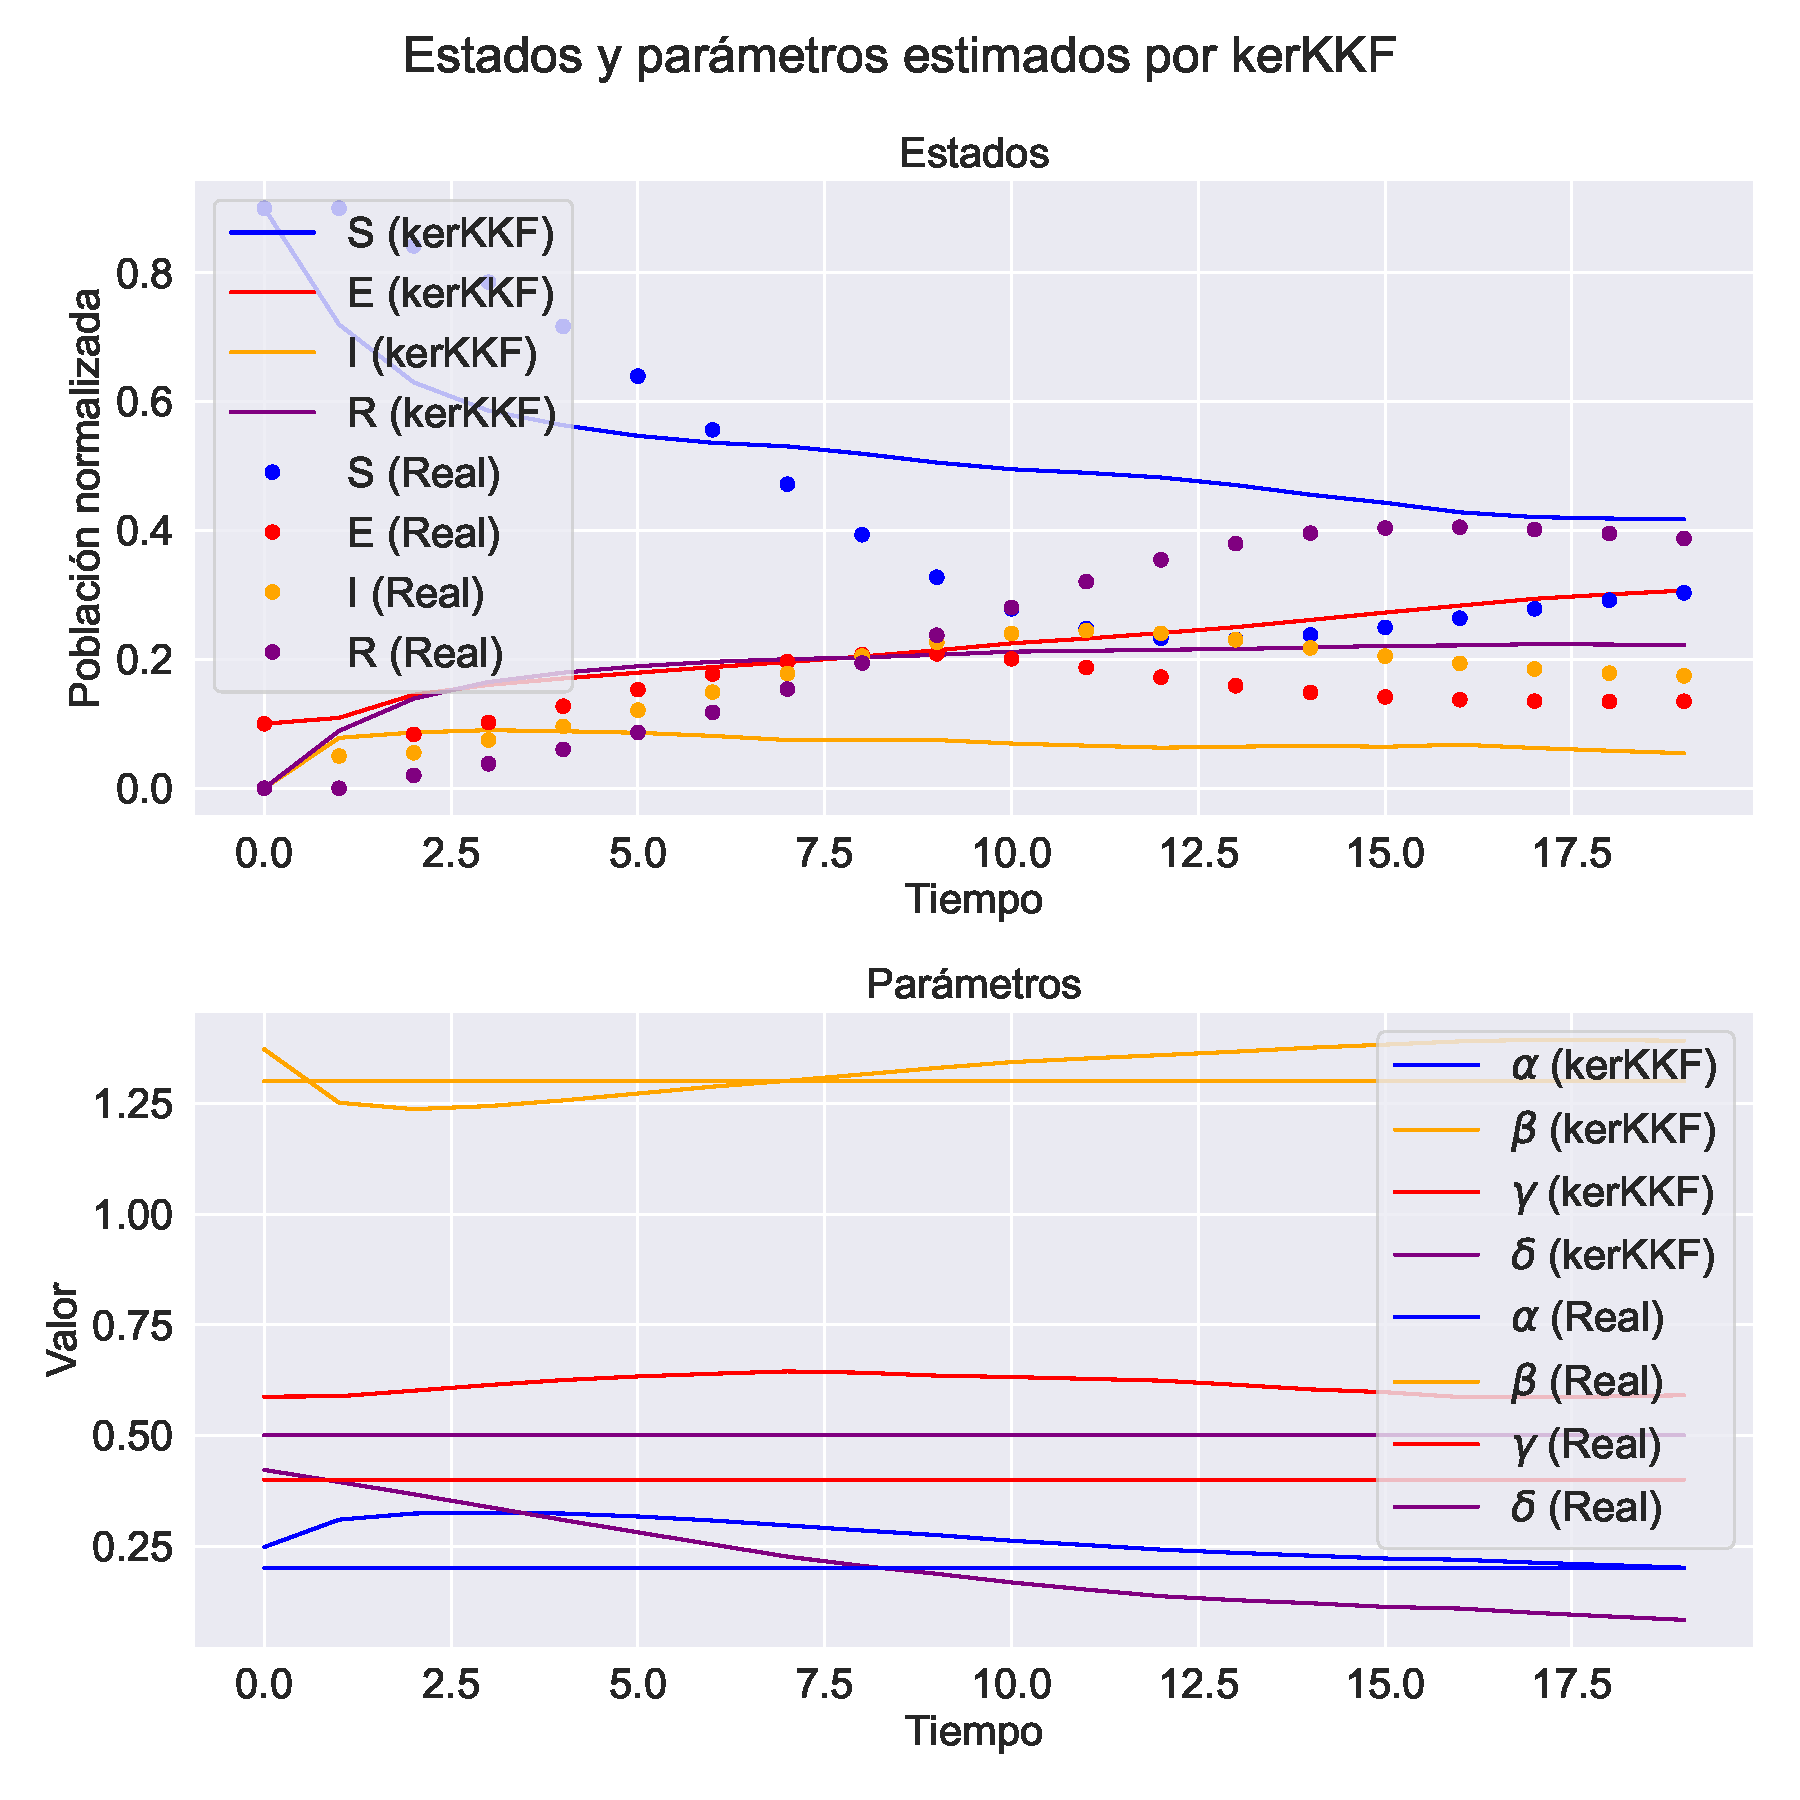
\includegraphics[height=\linewidth]{img/content/chapter4/nonlinear_filters_seir_params.pdf}
         \caption{}
         \label{fig:nonlinear_filters_sir_rec_params}
    \end{subfigure}
    \begin{subfigure}[b]{0.49\textwidth}
         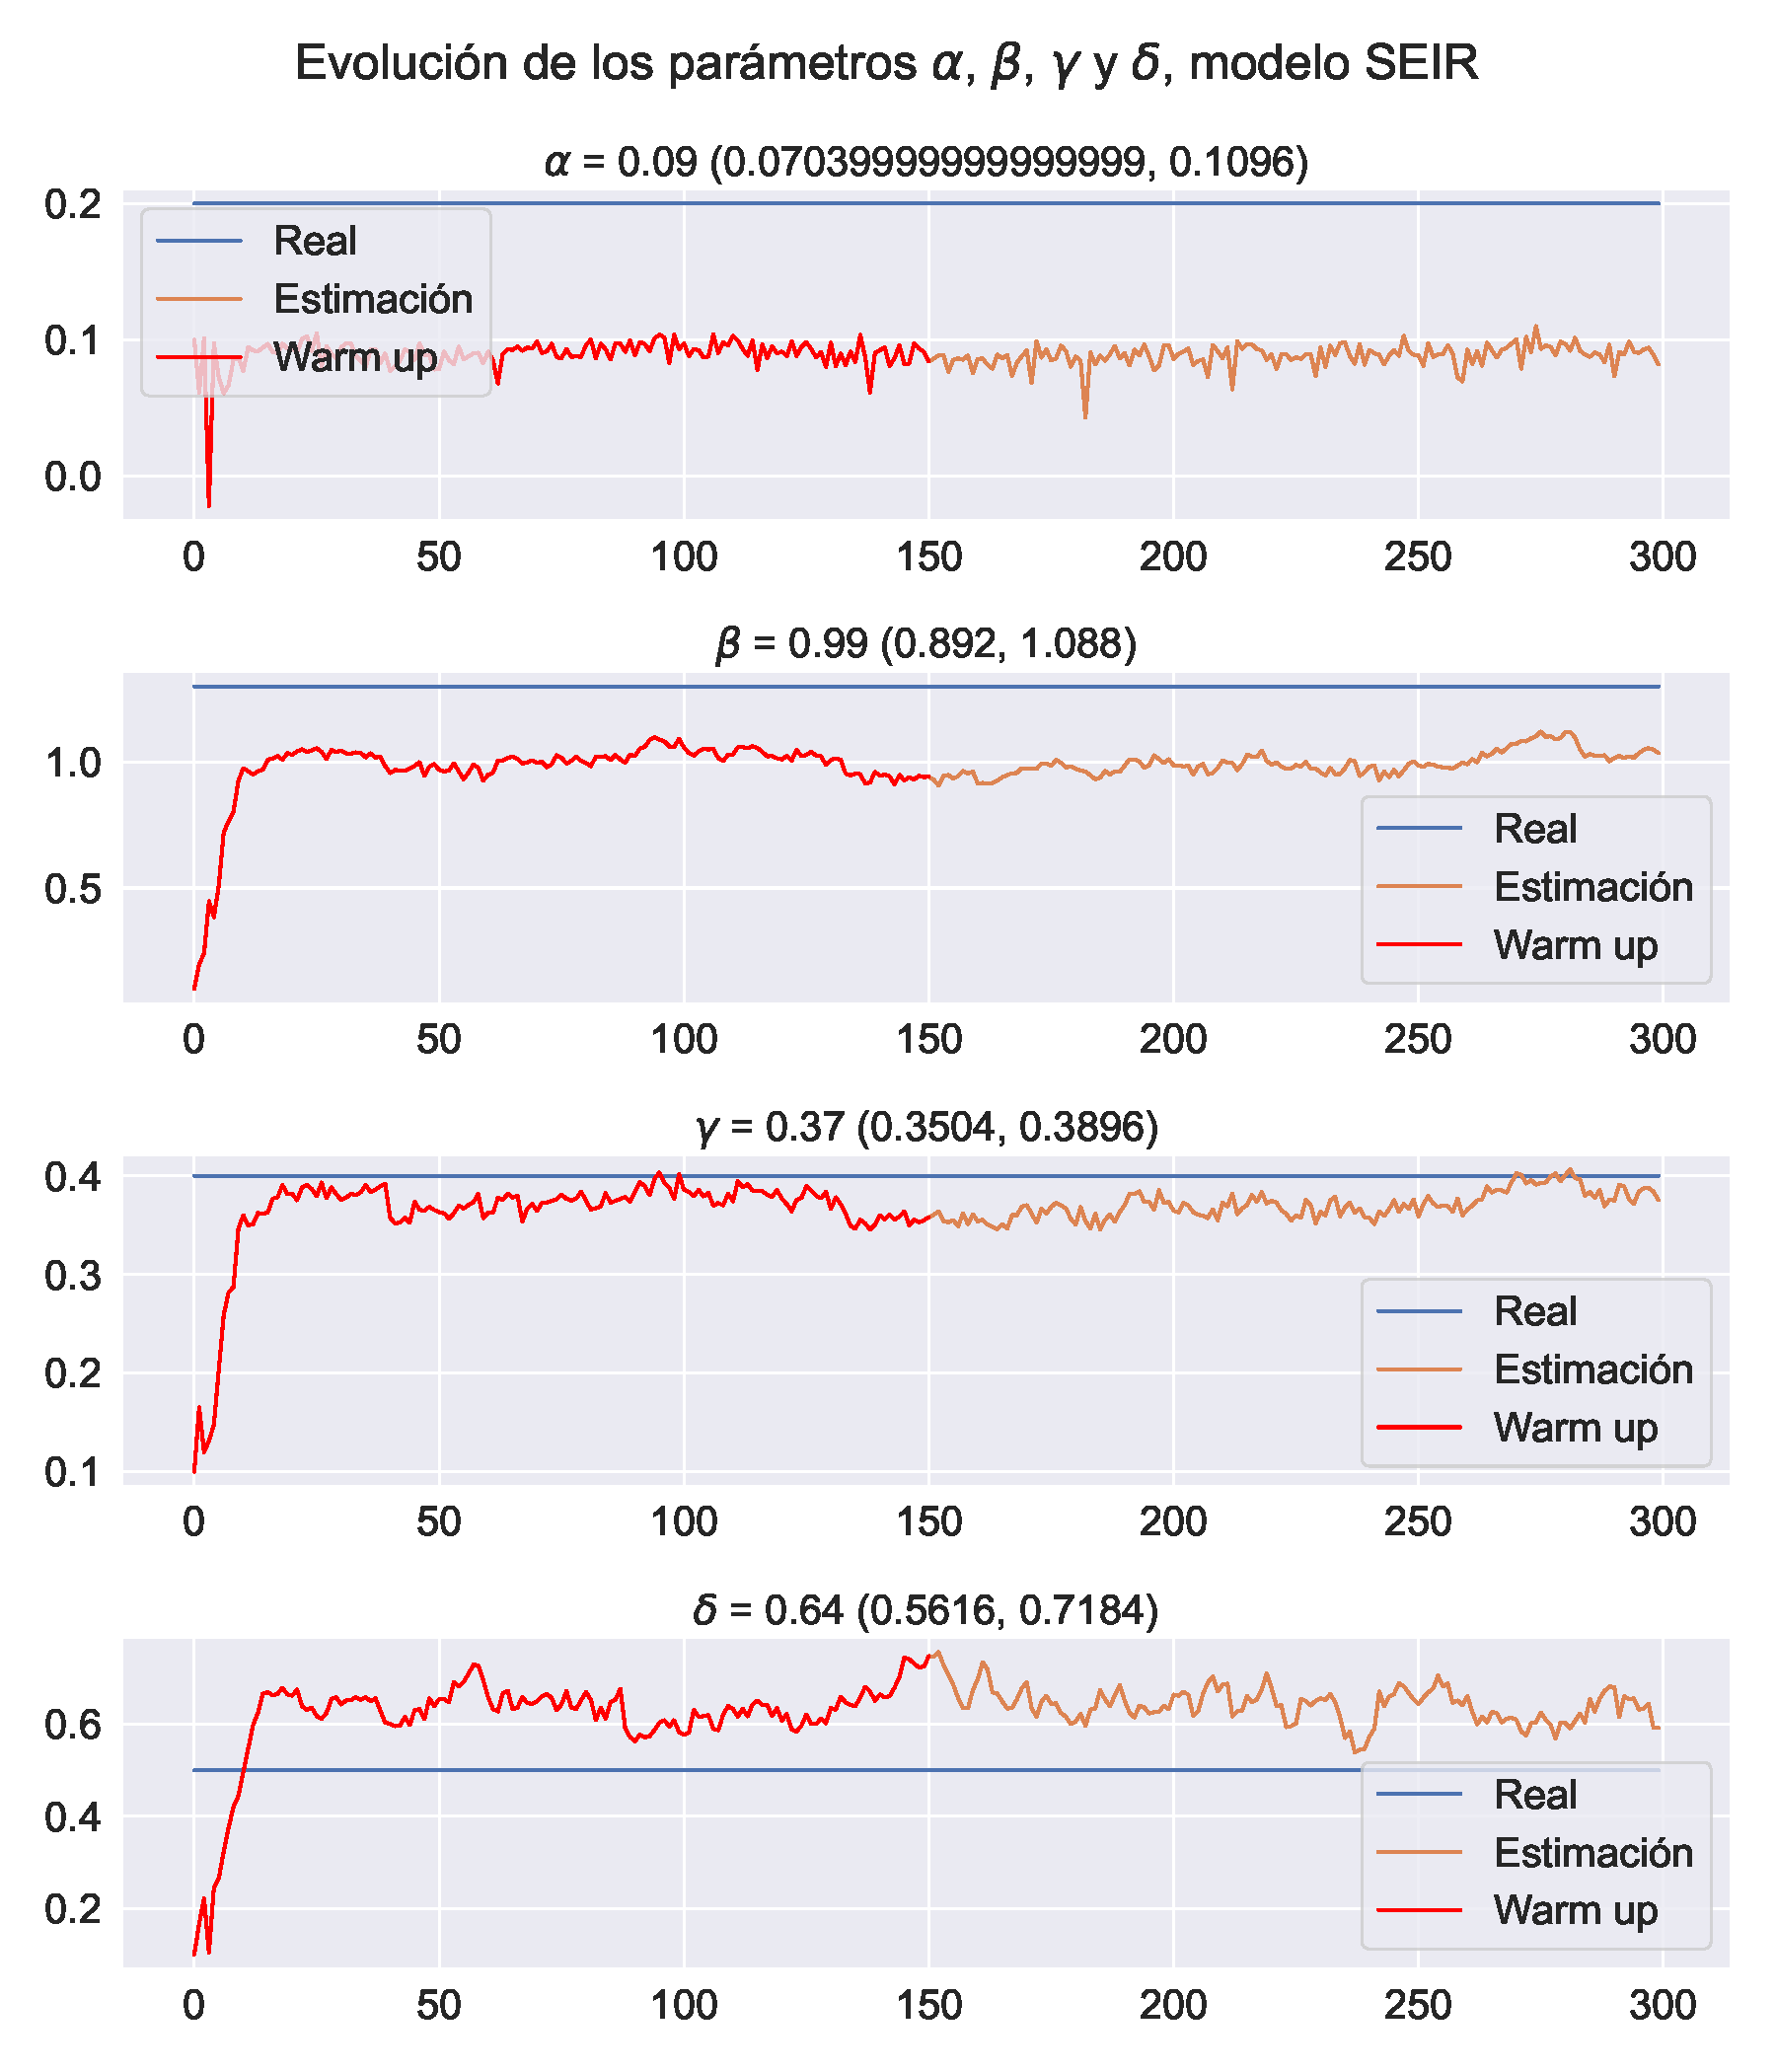
\includegraphics[height=\linewidth]{img/content/chapter4/nonlinear_filters_seir_params_evolution.pdf}
         \caption{}
         \label{fig:nonlinear_filters_seir_params_evolution}
    \end{subfigure}
    \caption{Resultado para modelo SEIR \eqref{eq:SEIR}. \\
    (a) Resultado de kerKKF para estimación de parámetros, primera cadena. \\
    (b) Evolución de la estimación de los parámetros a través de las iteraciones del algoritmo de estimación, primera cadena. De color rojo, el régimen de \textit{warm up}, mientras que en naranja se encuentran que sí serán consideradas para la estimación. En azul se encuentra el valor real del parámetro.}
    \label{fig:SEIR}
\end{figure}

\begin{figure}[h]
    \centering
    \begin{subfigure}[b]{0.8\textwidth}
        \centering 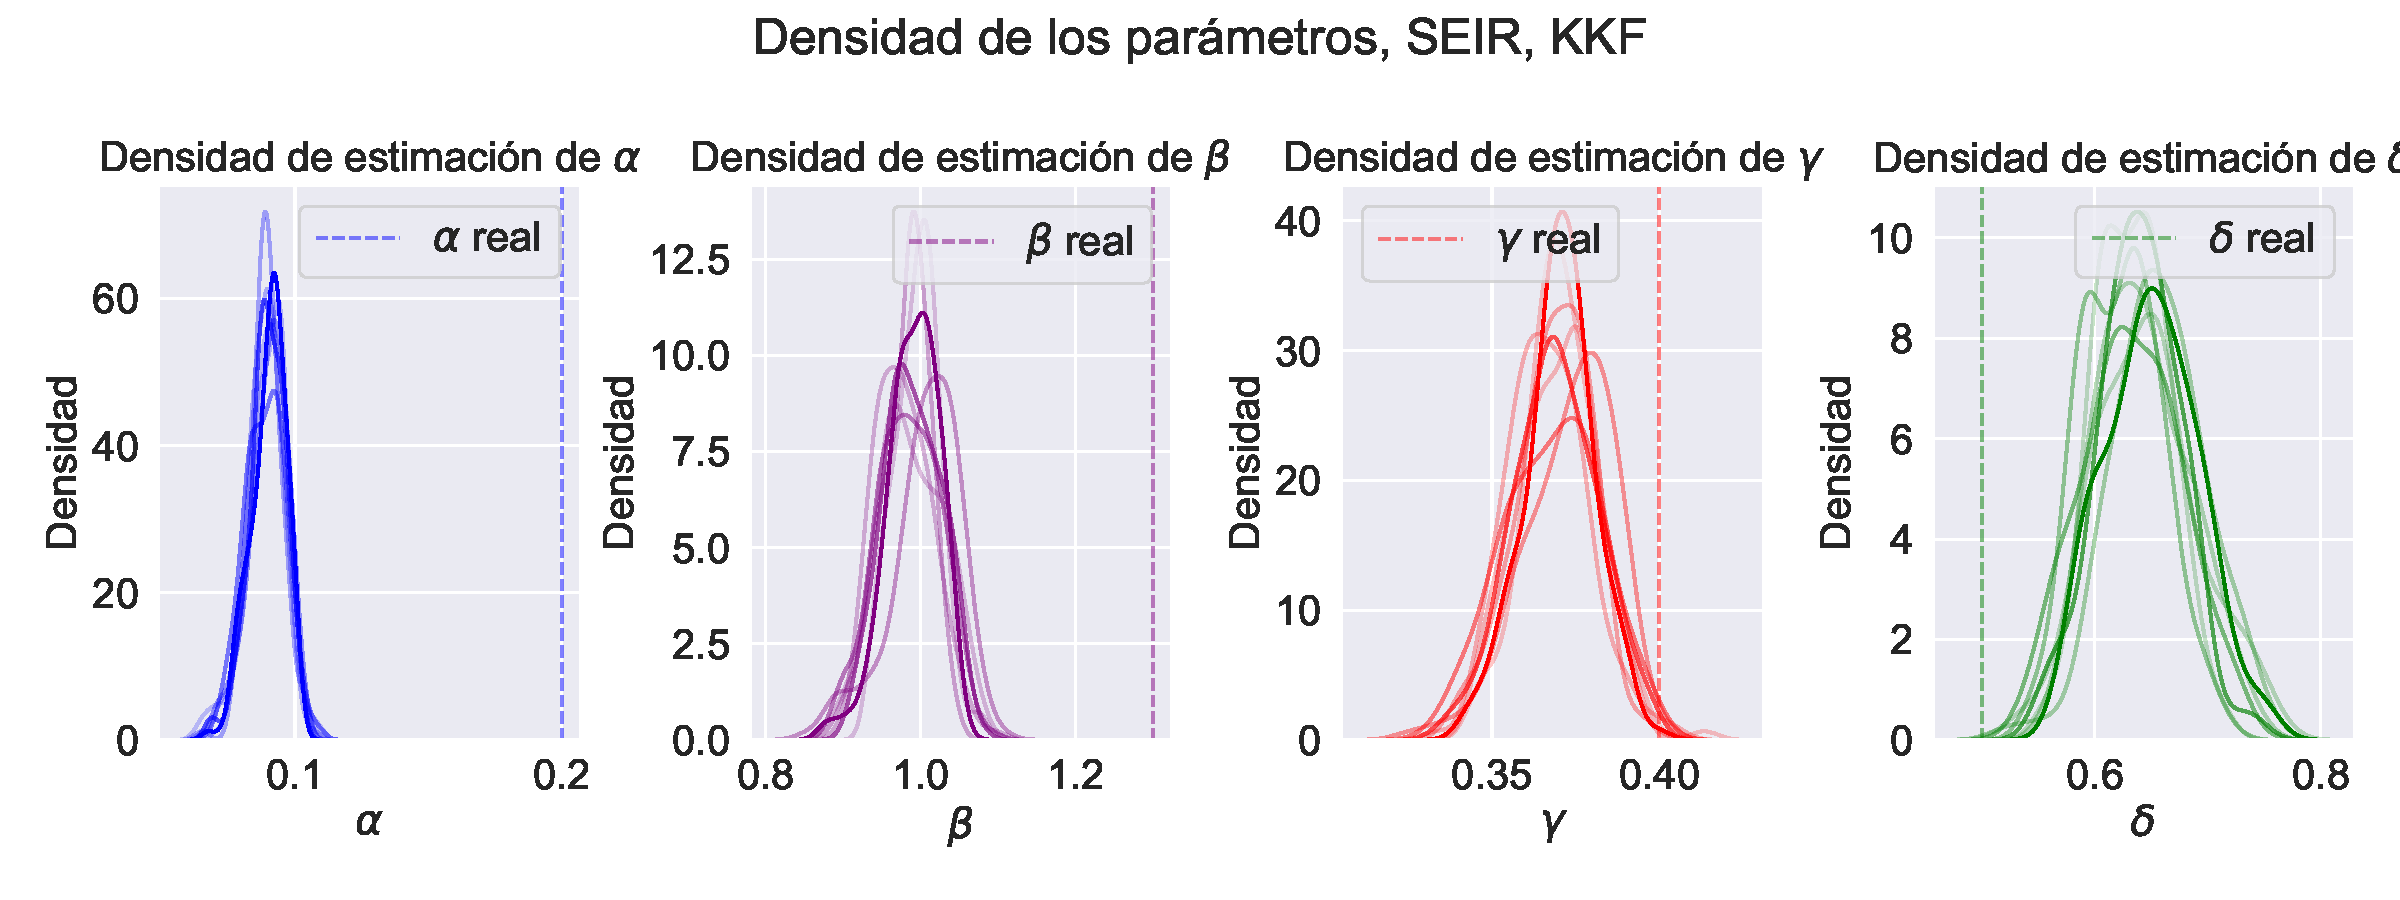
\includegraphics[width=0.9\linewidth]{img/content/chapter4/nonlinear_filters_seir_params_density.pdf}
    \caption{Densidades de las 8 cadenas.}
    \label{fig:nonlinear_filters_seir_params_density}
    \end{subfigure}
    \begin{subfigure}[b]{0.8\textwidth}
        \centering 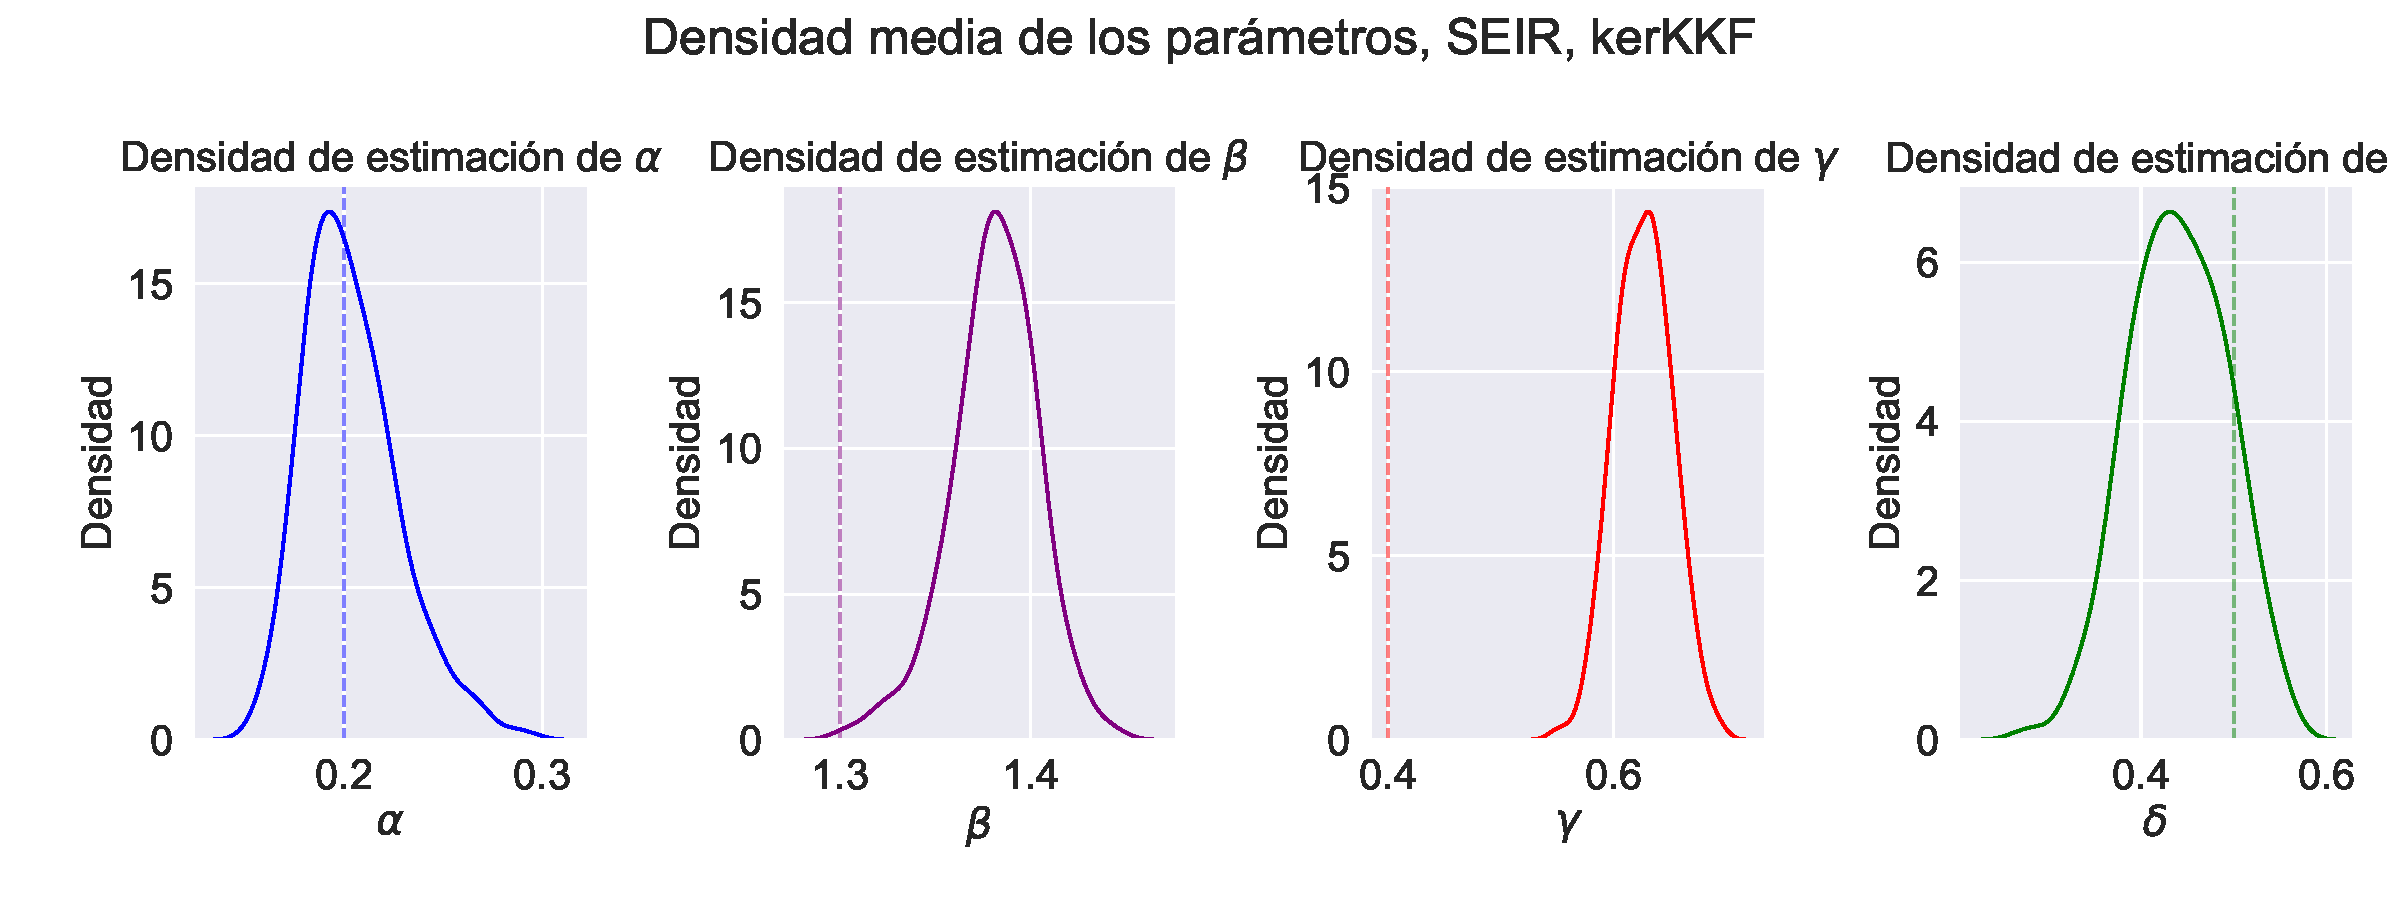
\includegraphics[width=0.9\linewidth]{img/content/chapter4/nonlinear_filters_seir_params_density_mean.pdf}
    \caption{Densidad promedio entre las 8 cadenas.}
    \label{fig:nonlinear_filters_seir_params_density_mean}
    \end{subfigure}
    \caption{Densidades de estimación para los parámetros del modelo SEIR.}
\end{figure}

\begin{figure}[h]
    \centering
    \begin{subfigure}[b]{0.49\linewidth}
        \centering 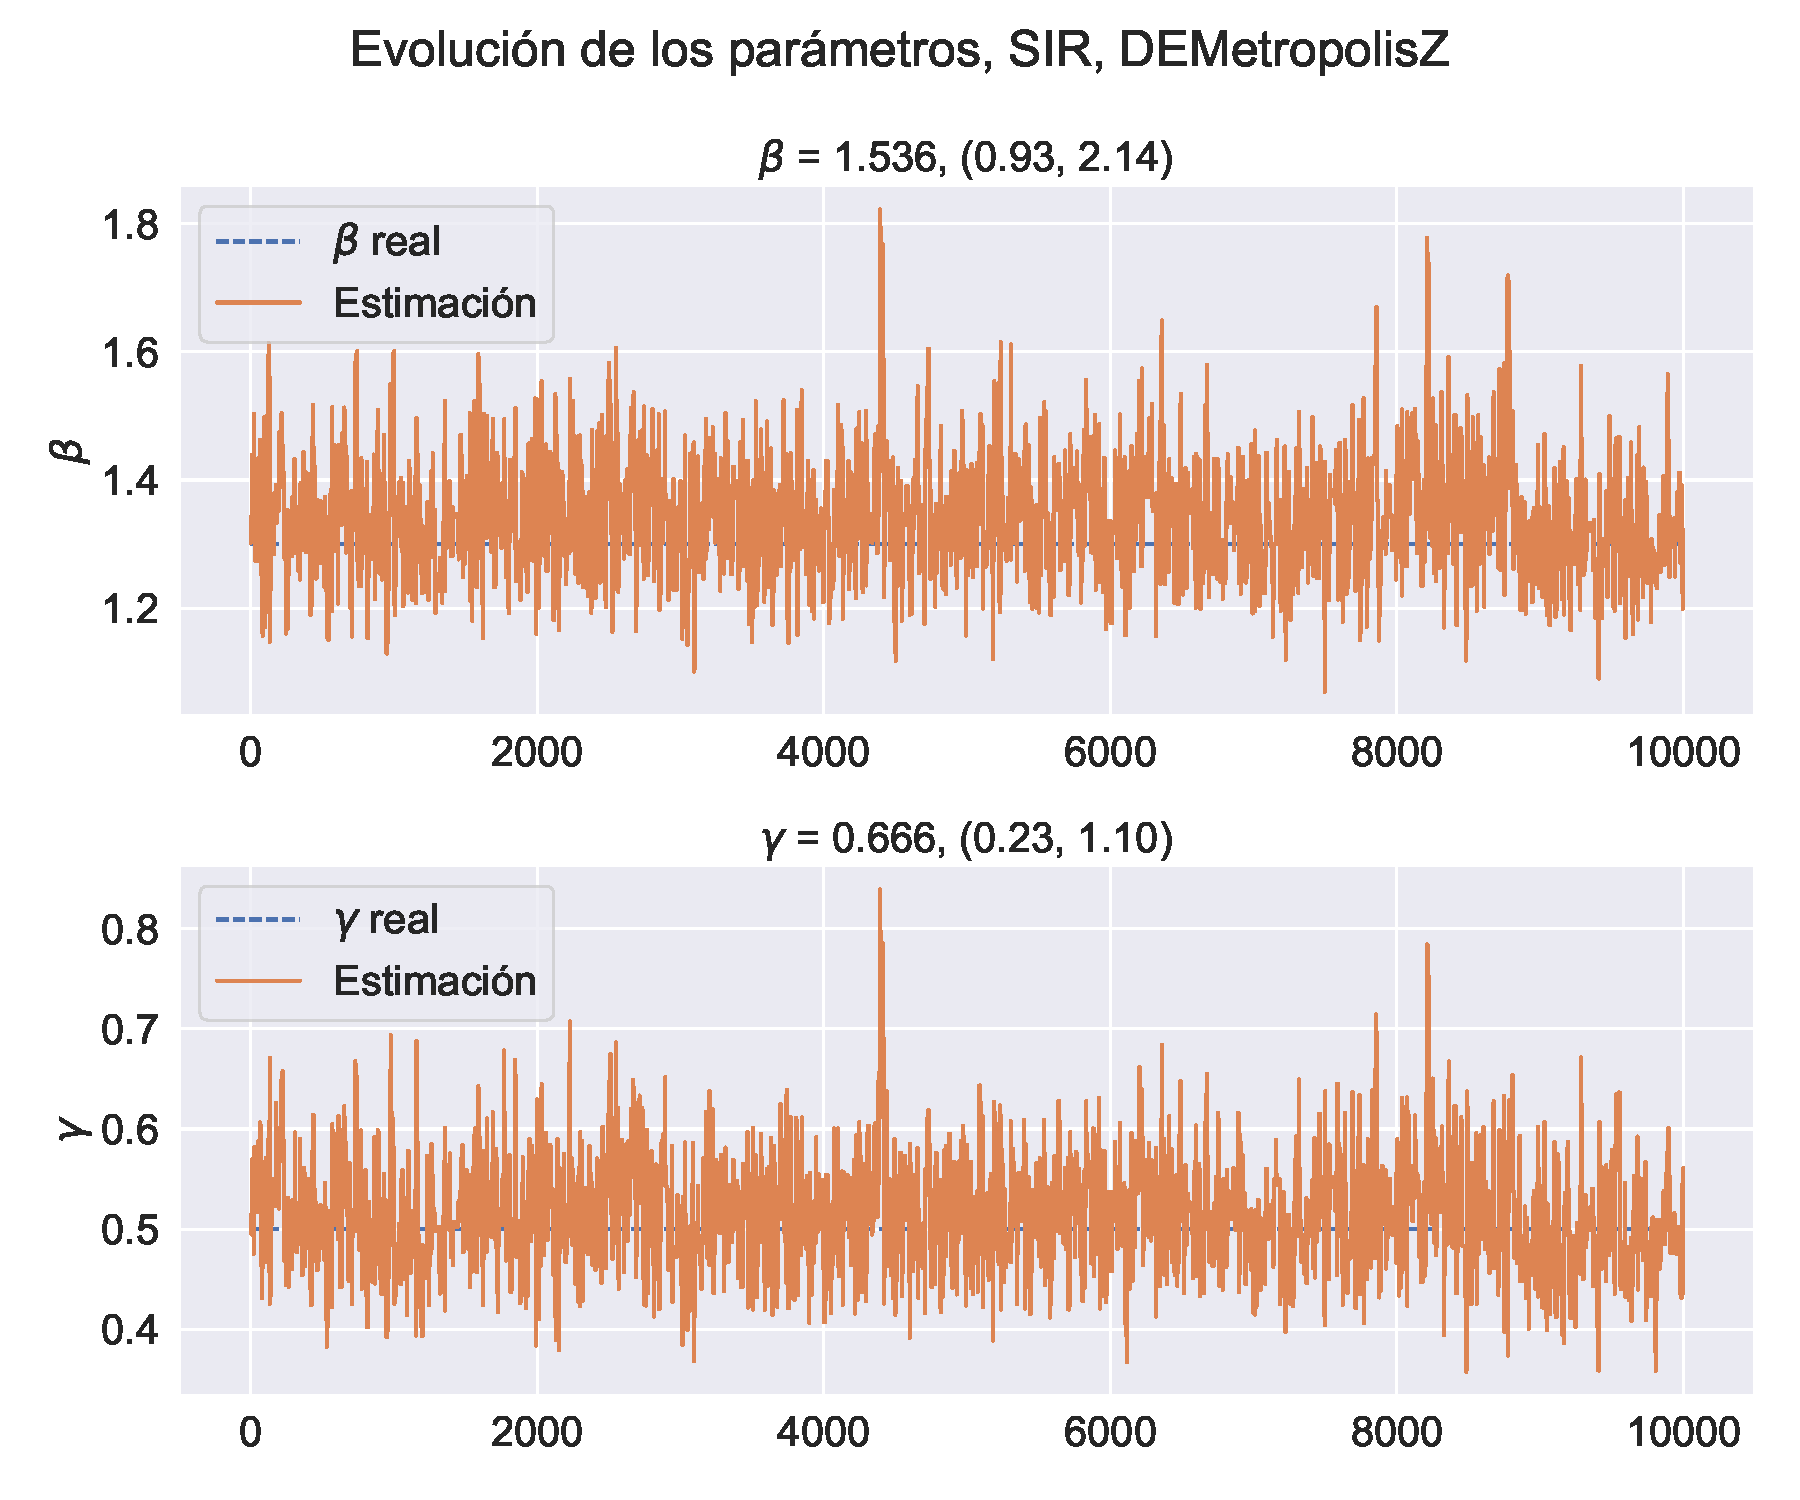
\includegraphics[height=0.65\linewidth]{img/content/chapter4/DEMetropolis_sir_params_trace.pdf}
        \caption{DEMetropolisZ, 20000 iteraciones de estimación y 20000 de \textit{warm up}.}
        \label{fig:DEMetropolis_sir_rec_params_trace}
    \end{subfigure}
    \begin{subfigure}[b]{0.49\linewidth}
        \centering 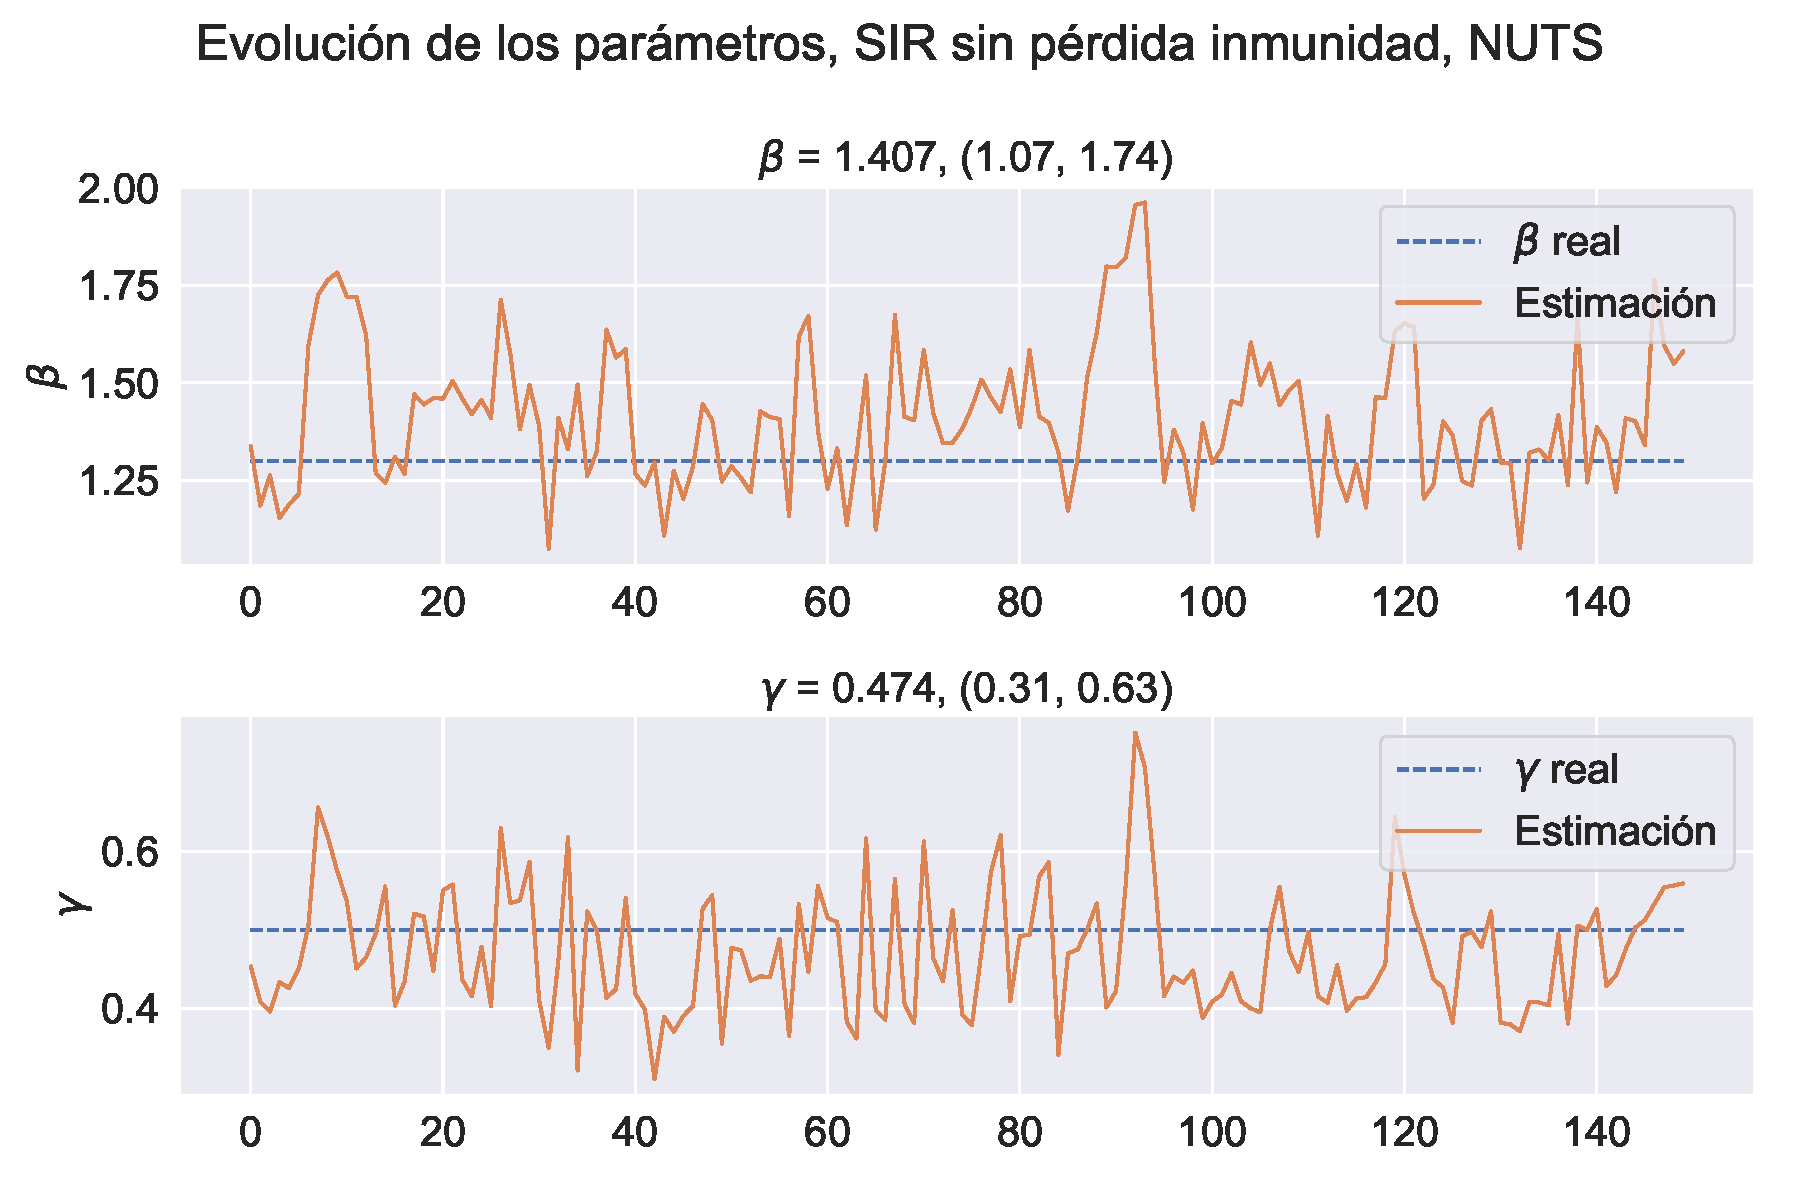
\includegraphics[height=0.65\linewidth]{img/content/chapter4/NUTS_sir_params_trace.pdf}
        \caption{NUTS, 150 iteraciones de estimación y 150 de \textit{warm up}.}
        \label{fig:NUTS_sir_params_trace}
    \end{subfigure}
    \caption{Evolución de los parámetros de SIR para una cadena de MCMC. Se muestran las iteraciones posteriores a las de \textit{warm up}, en naranjo el valor estimado del parámetro y en línea punteada el valor real.}
    \label{fig:MCMC_sir_params_trace}
\end{figure}

\begin{figure}[h]
    \centering
    \begin{subfigure}[b]{\linewidth}
        \centering
        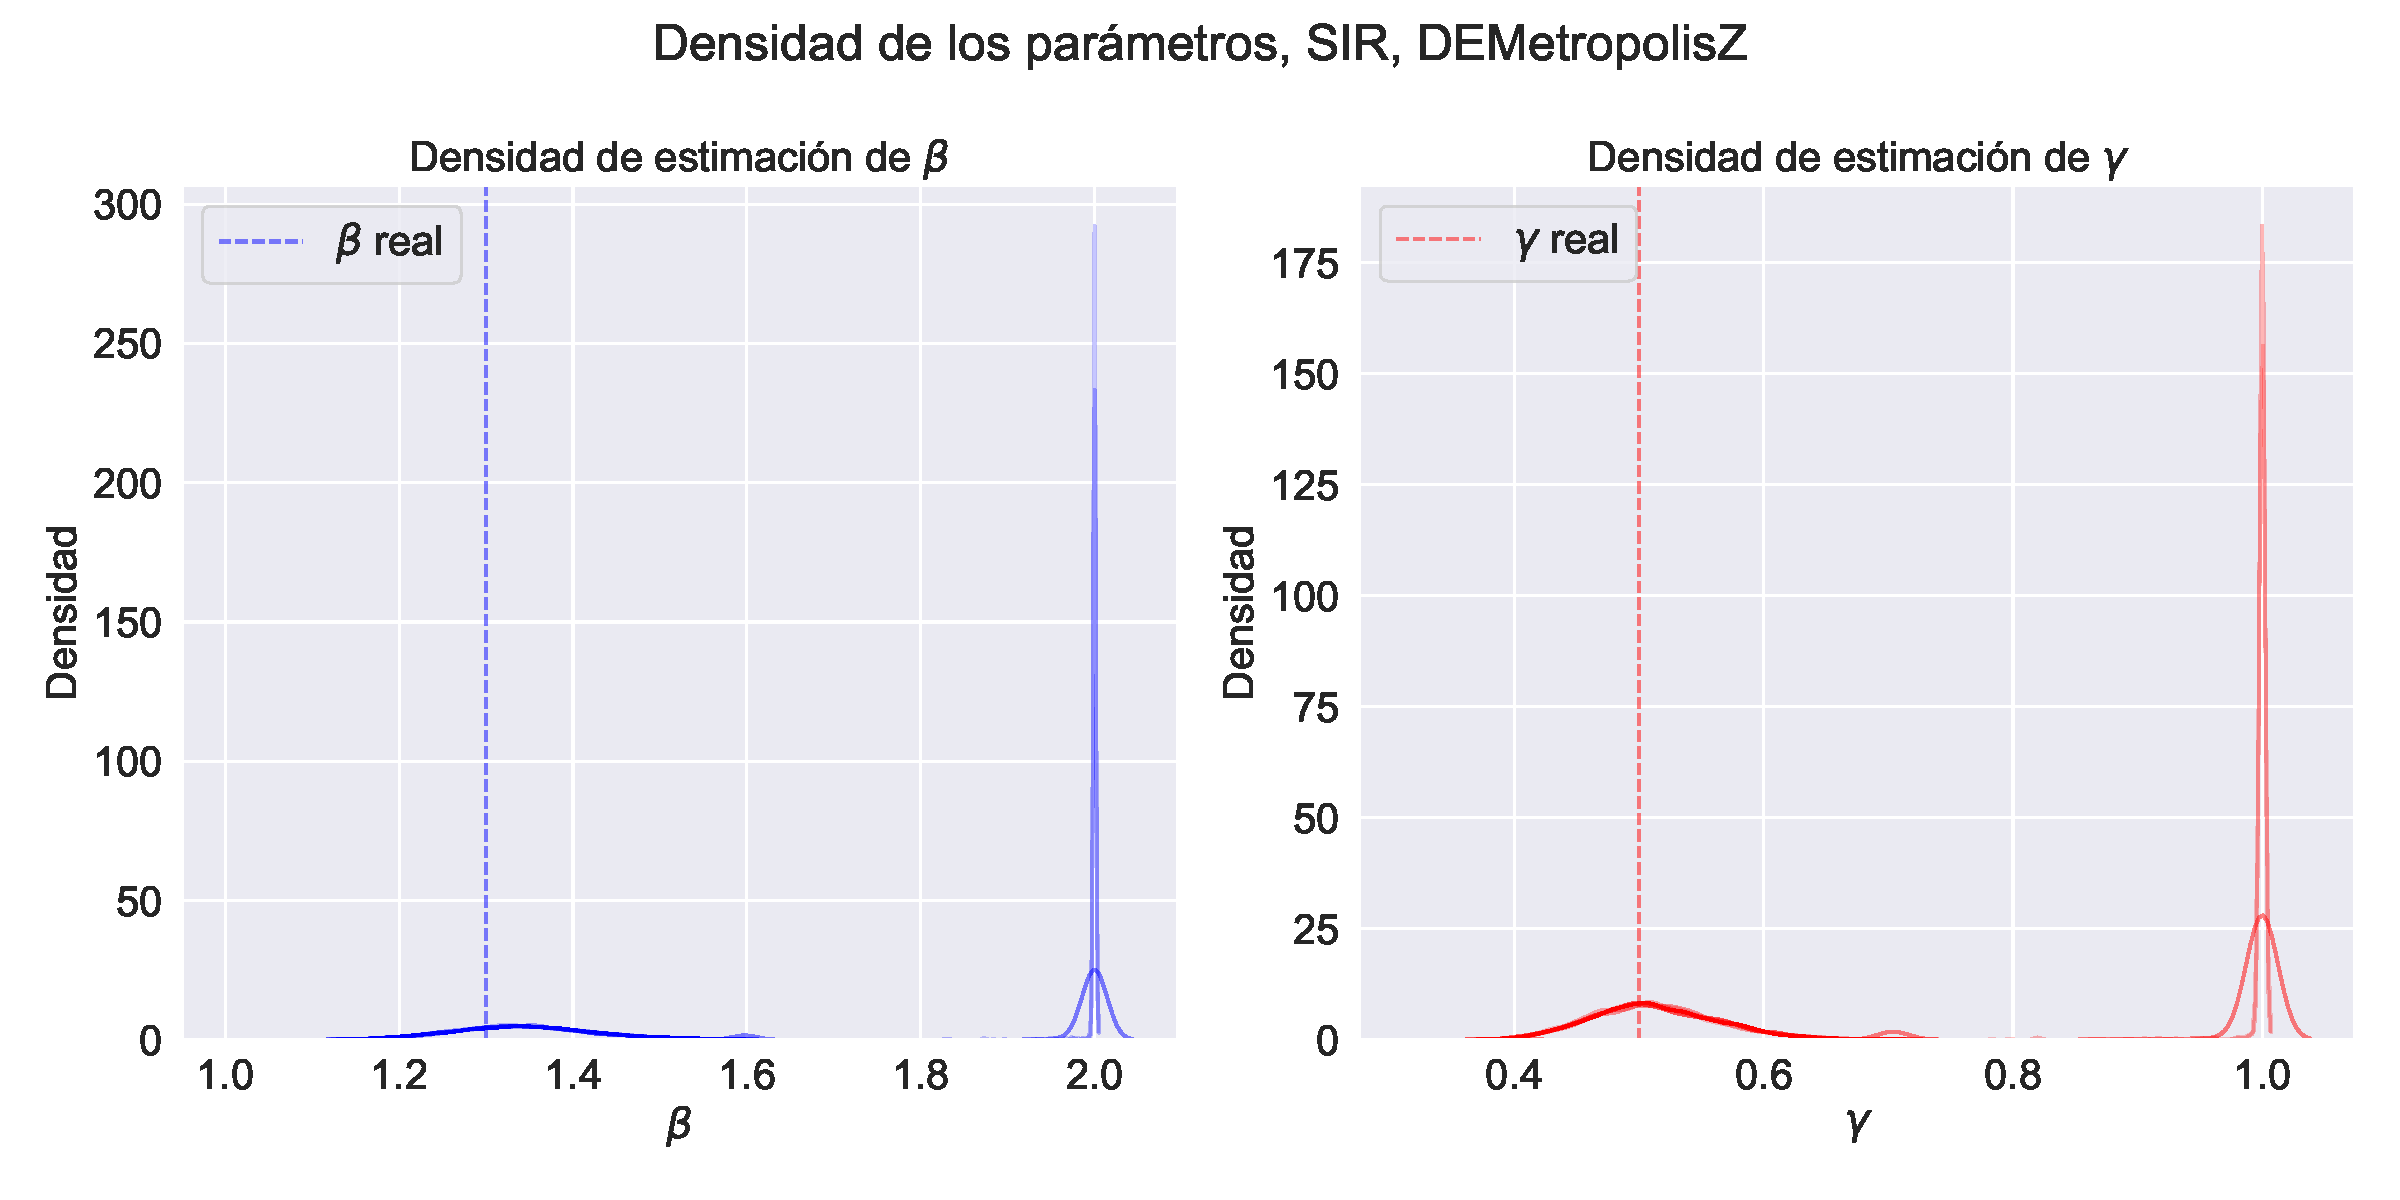
\includegraphics[width=0.7\linewidth]{img/content/chapter4/DEMetropolis_sir_params_density.pdf}
        \caption{Densidad de las 8 cadenas.}
    \end{subfigure}
     \begin{subfigure}[b]{\linewidth}
        \centering
        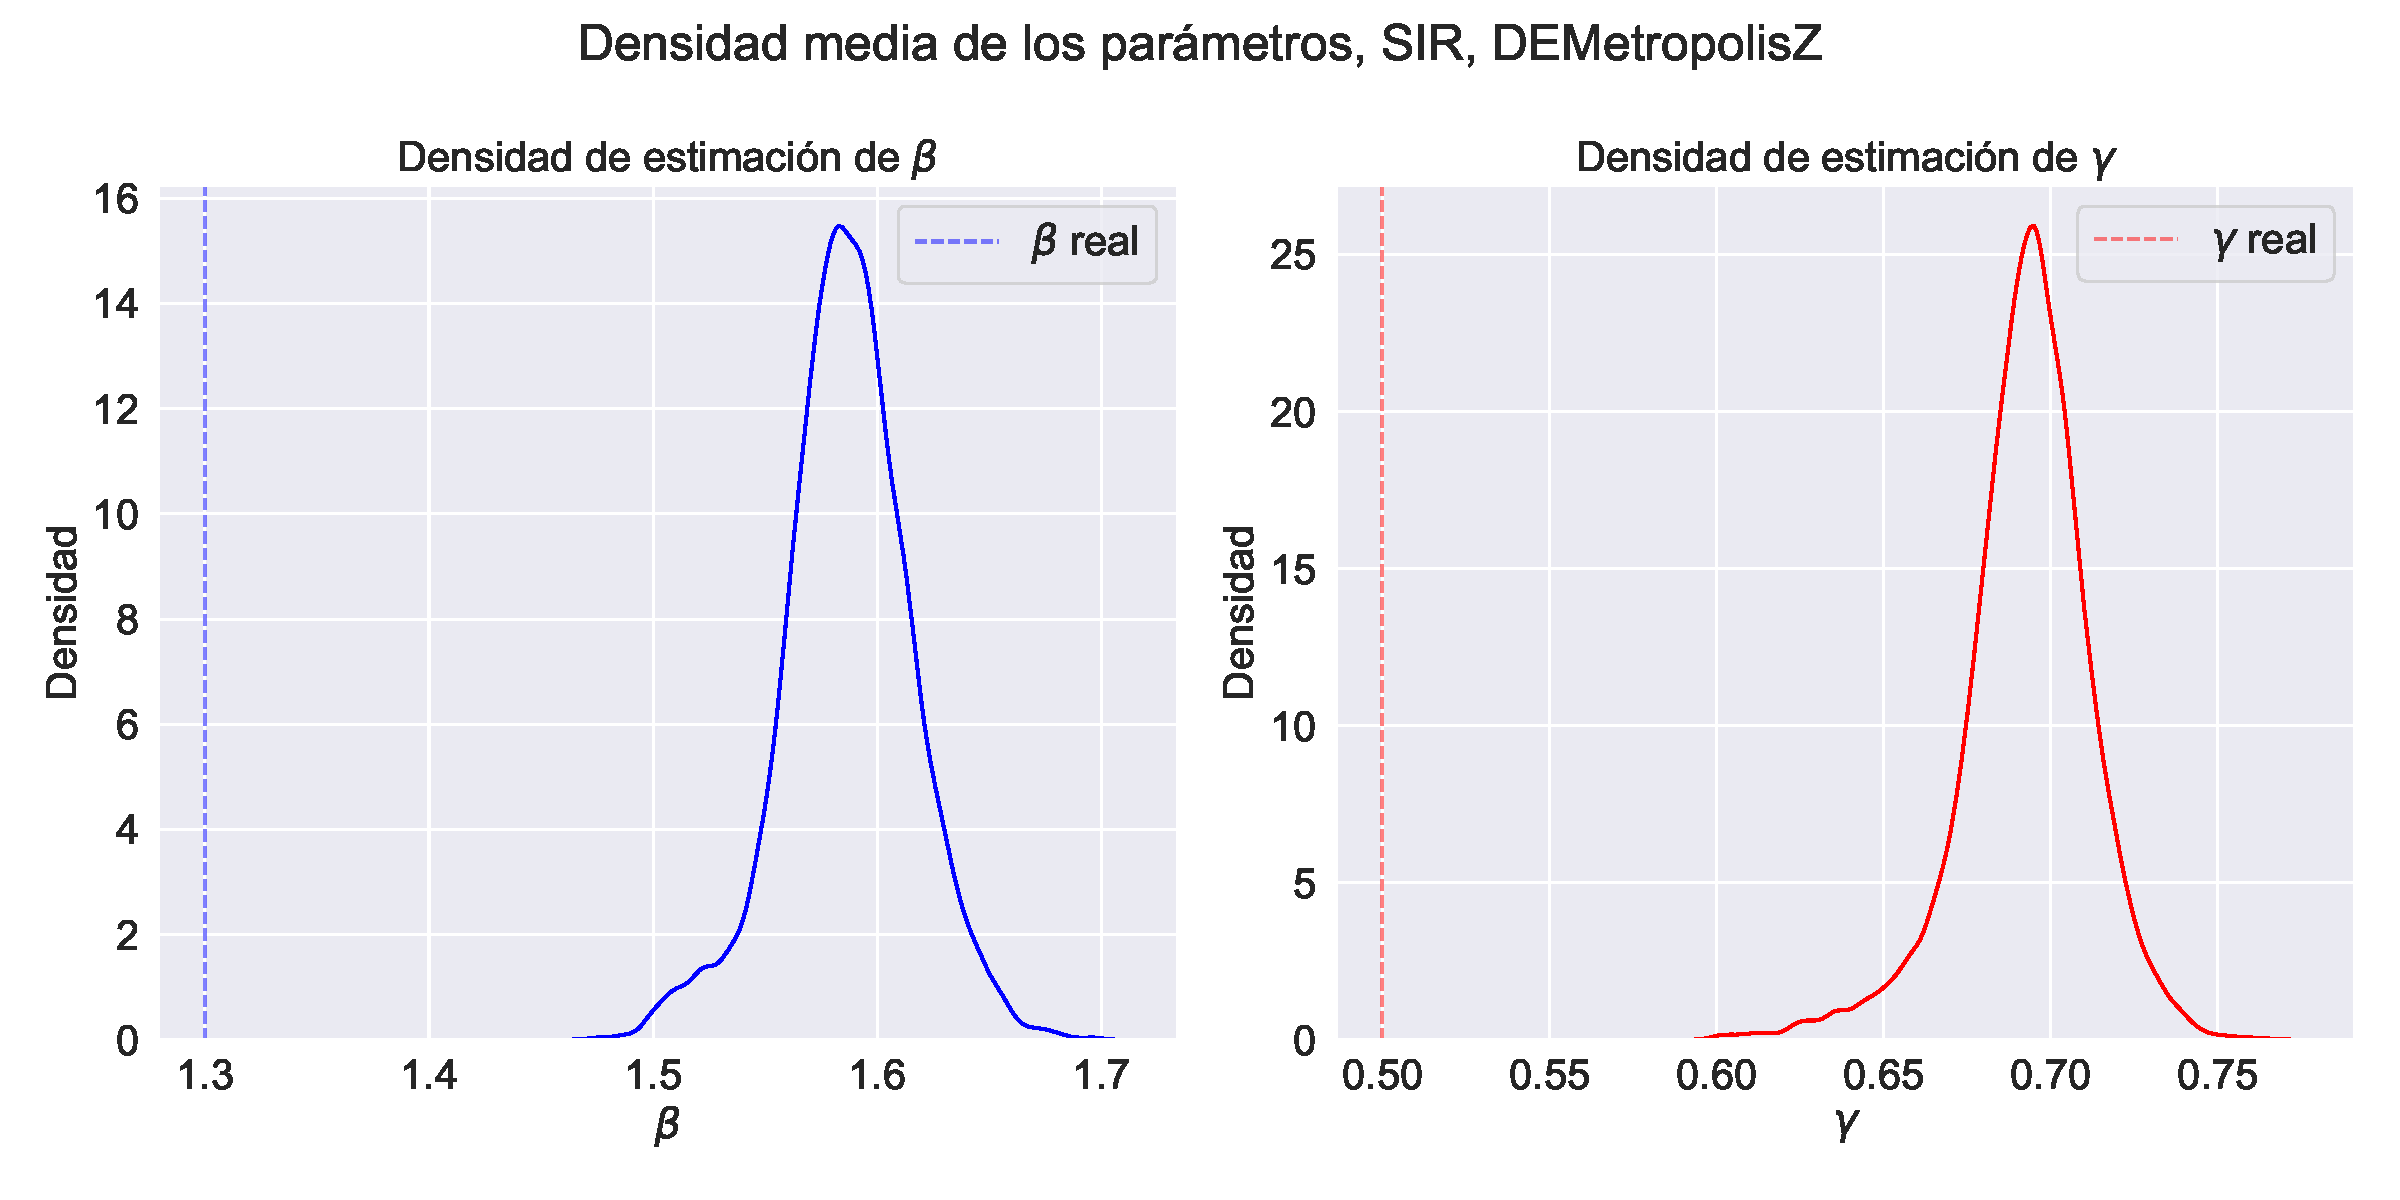
\includegraphics[width=0.7\linewidth]{img/content/chapter4/DEMetropolis_sir_params_density_mean.pdf}
        \caption{Densidad de las 8 cadenas.}
    \end{subfigure}
    \caption{Densidad de los parámetros del modelo SIR estimados con MCMC con \textit{sampler} DEMEtropolisZ.}
\end{figure}

\begin{figure}[h]
    \centering
    \begin{subfigure}[b]{\linewidth}
        \centering
        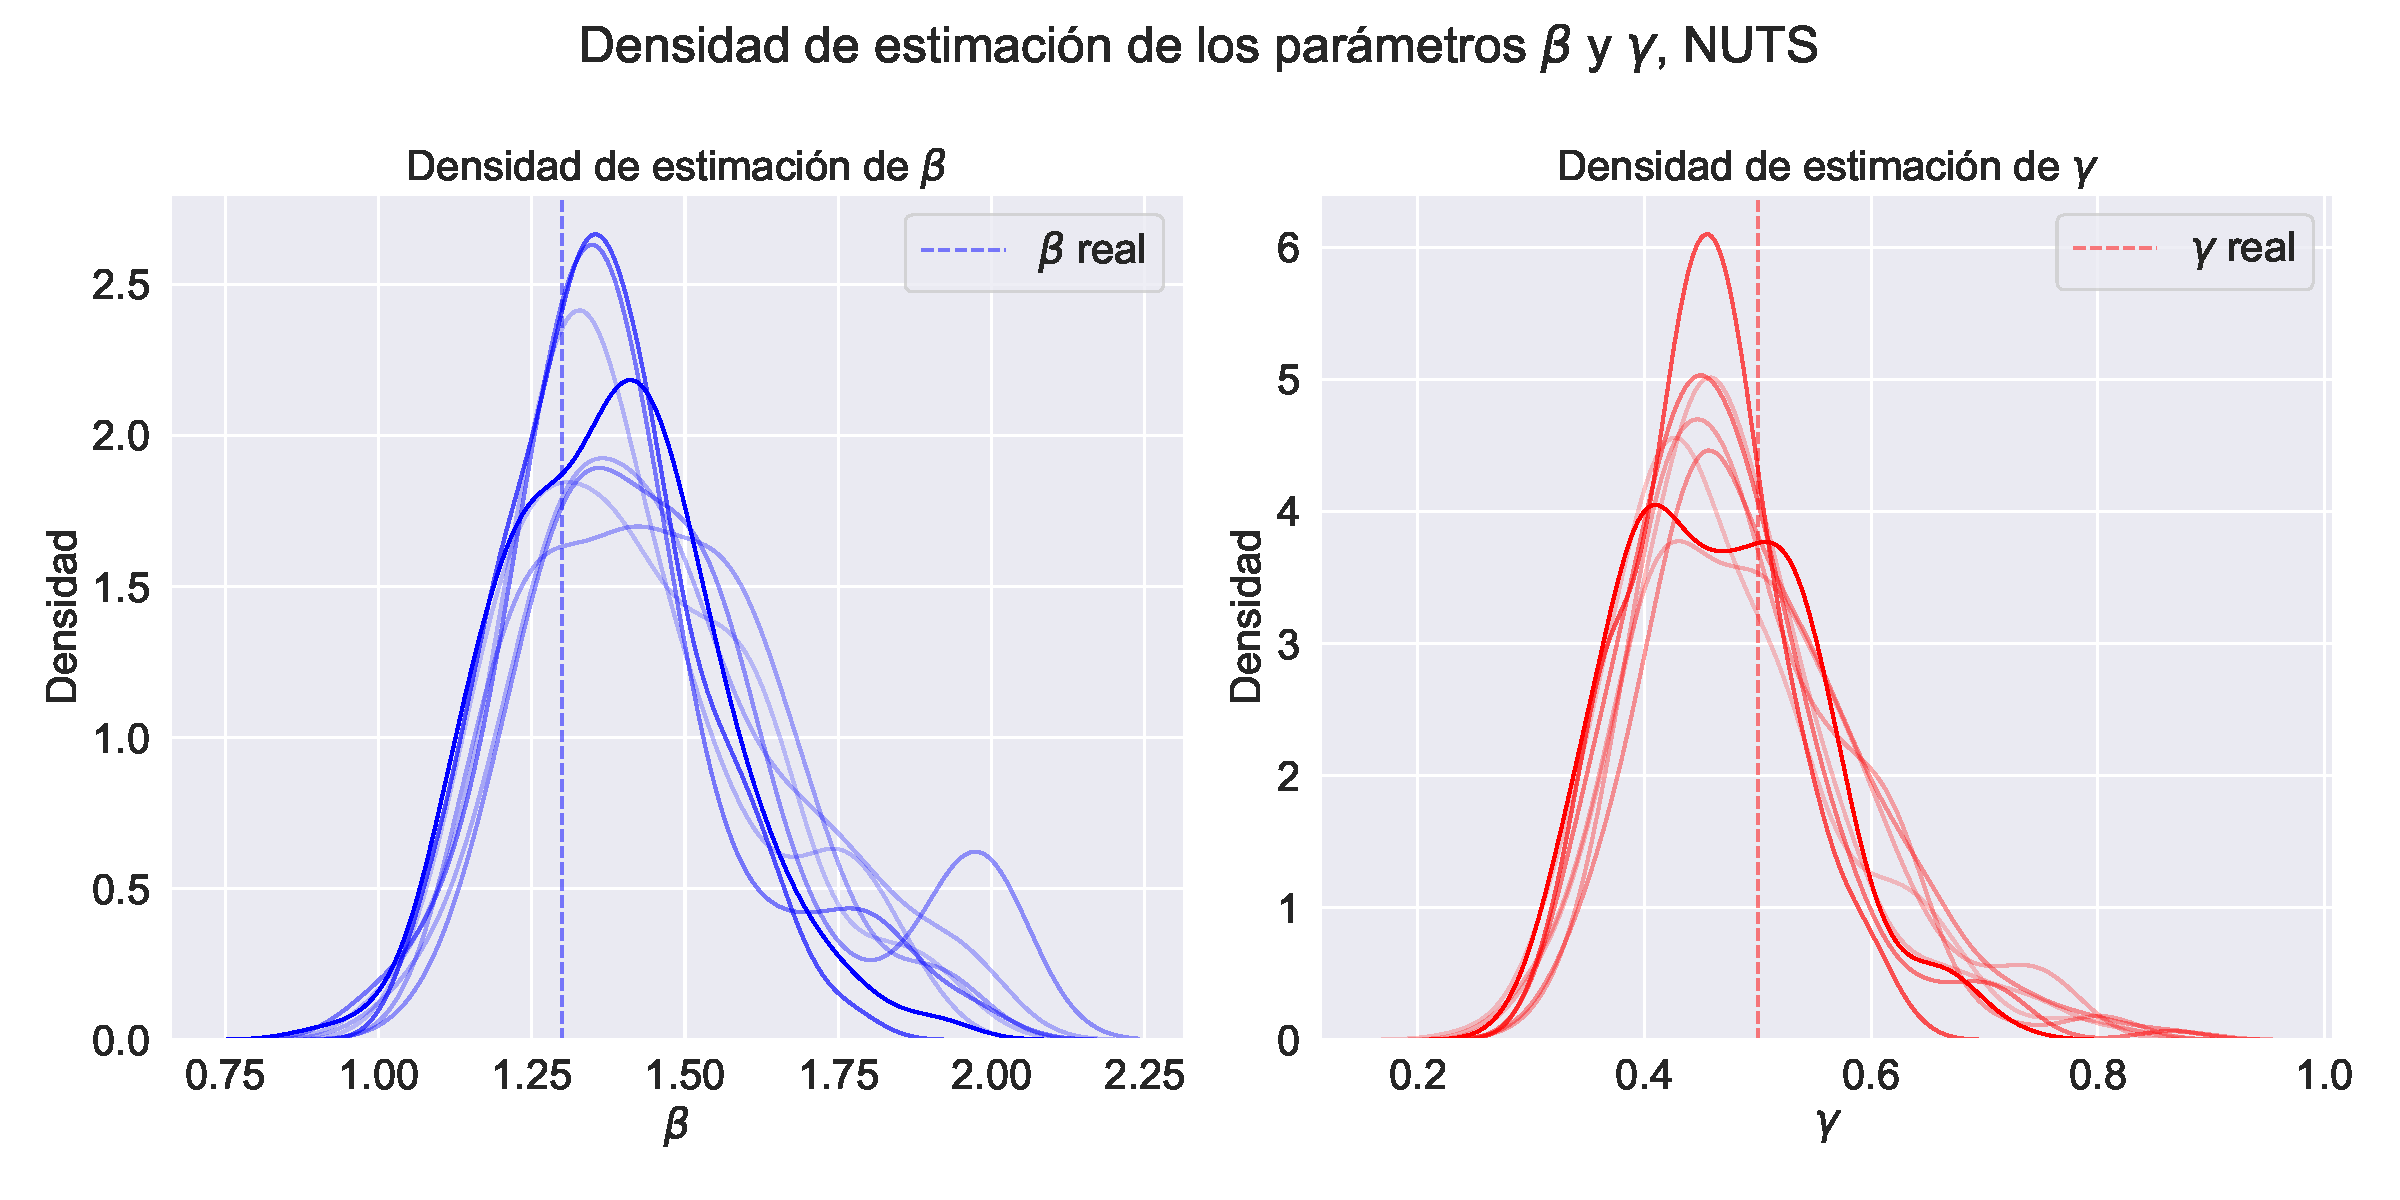
\includegraphics[width=0.55\linewidth]{img/content/chapter4/NUTS_sir_params_density.pdf}
        \caption{Densidad de las 8 cadenas.}
    \end{subfigure}
     \begin{subfigure}[b]{\linewidth}
        \centering
        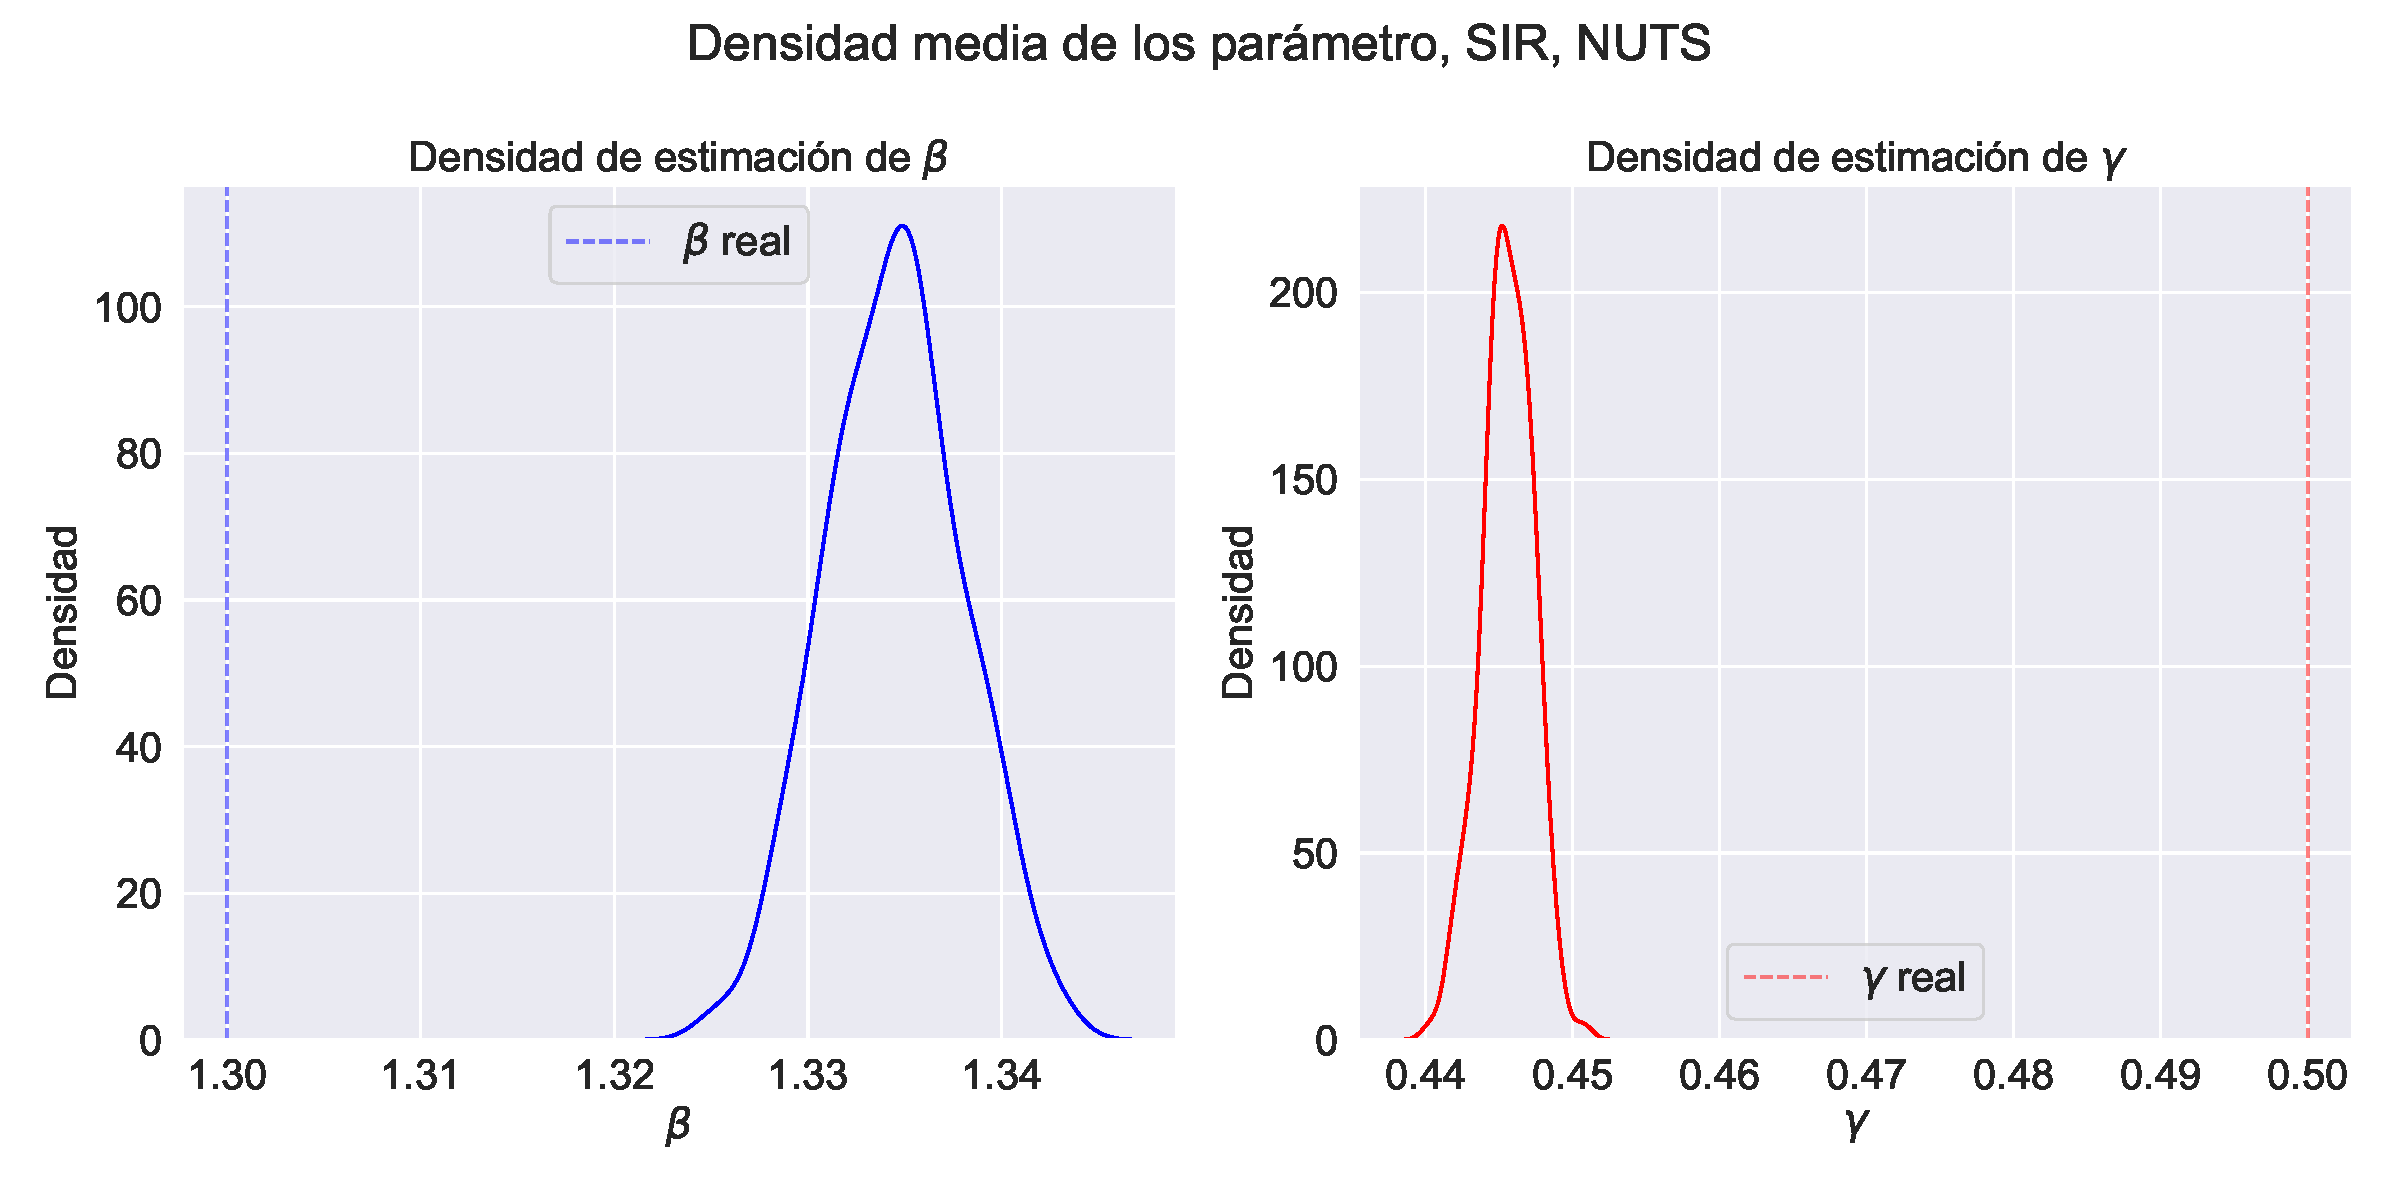
\includegraphics[width=0.55\linewidth]{img/content/chapter4/NUTS_sir_params_density_mean.pdf}
        \caption{Densidad de las 8 cadenas.}
    \end{subfigure}
    \caption{Densidad de los parámetros del modelo SIR estimados con MCMC con \textit{sampler} NUTS.}
\end{figure}

\begin{figure}[h]
    \centering
    \begin{subfigure}[b]{0.49\linewidth}
        \centering
        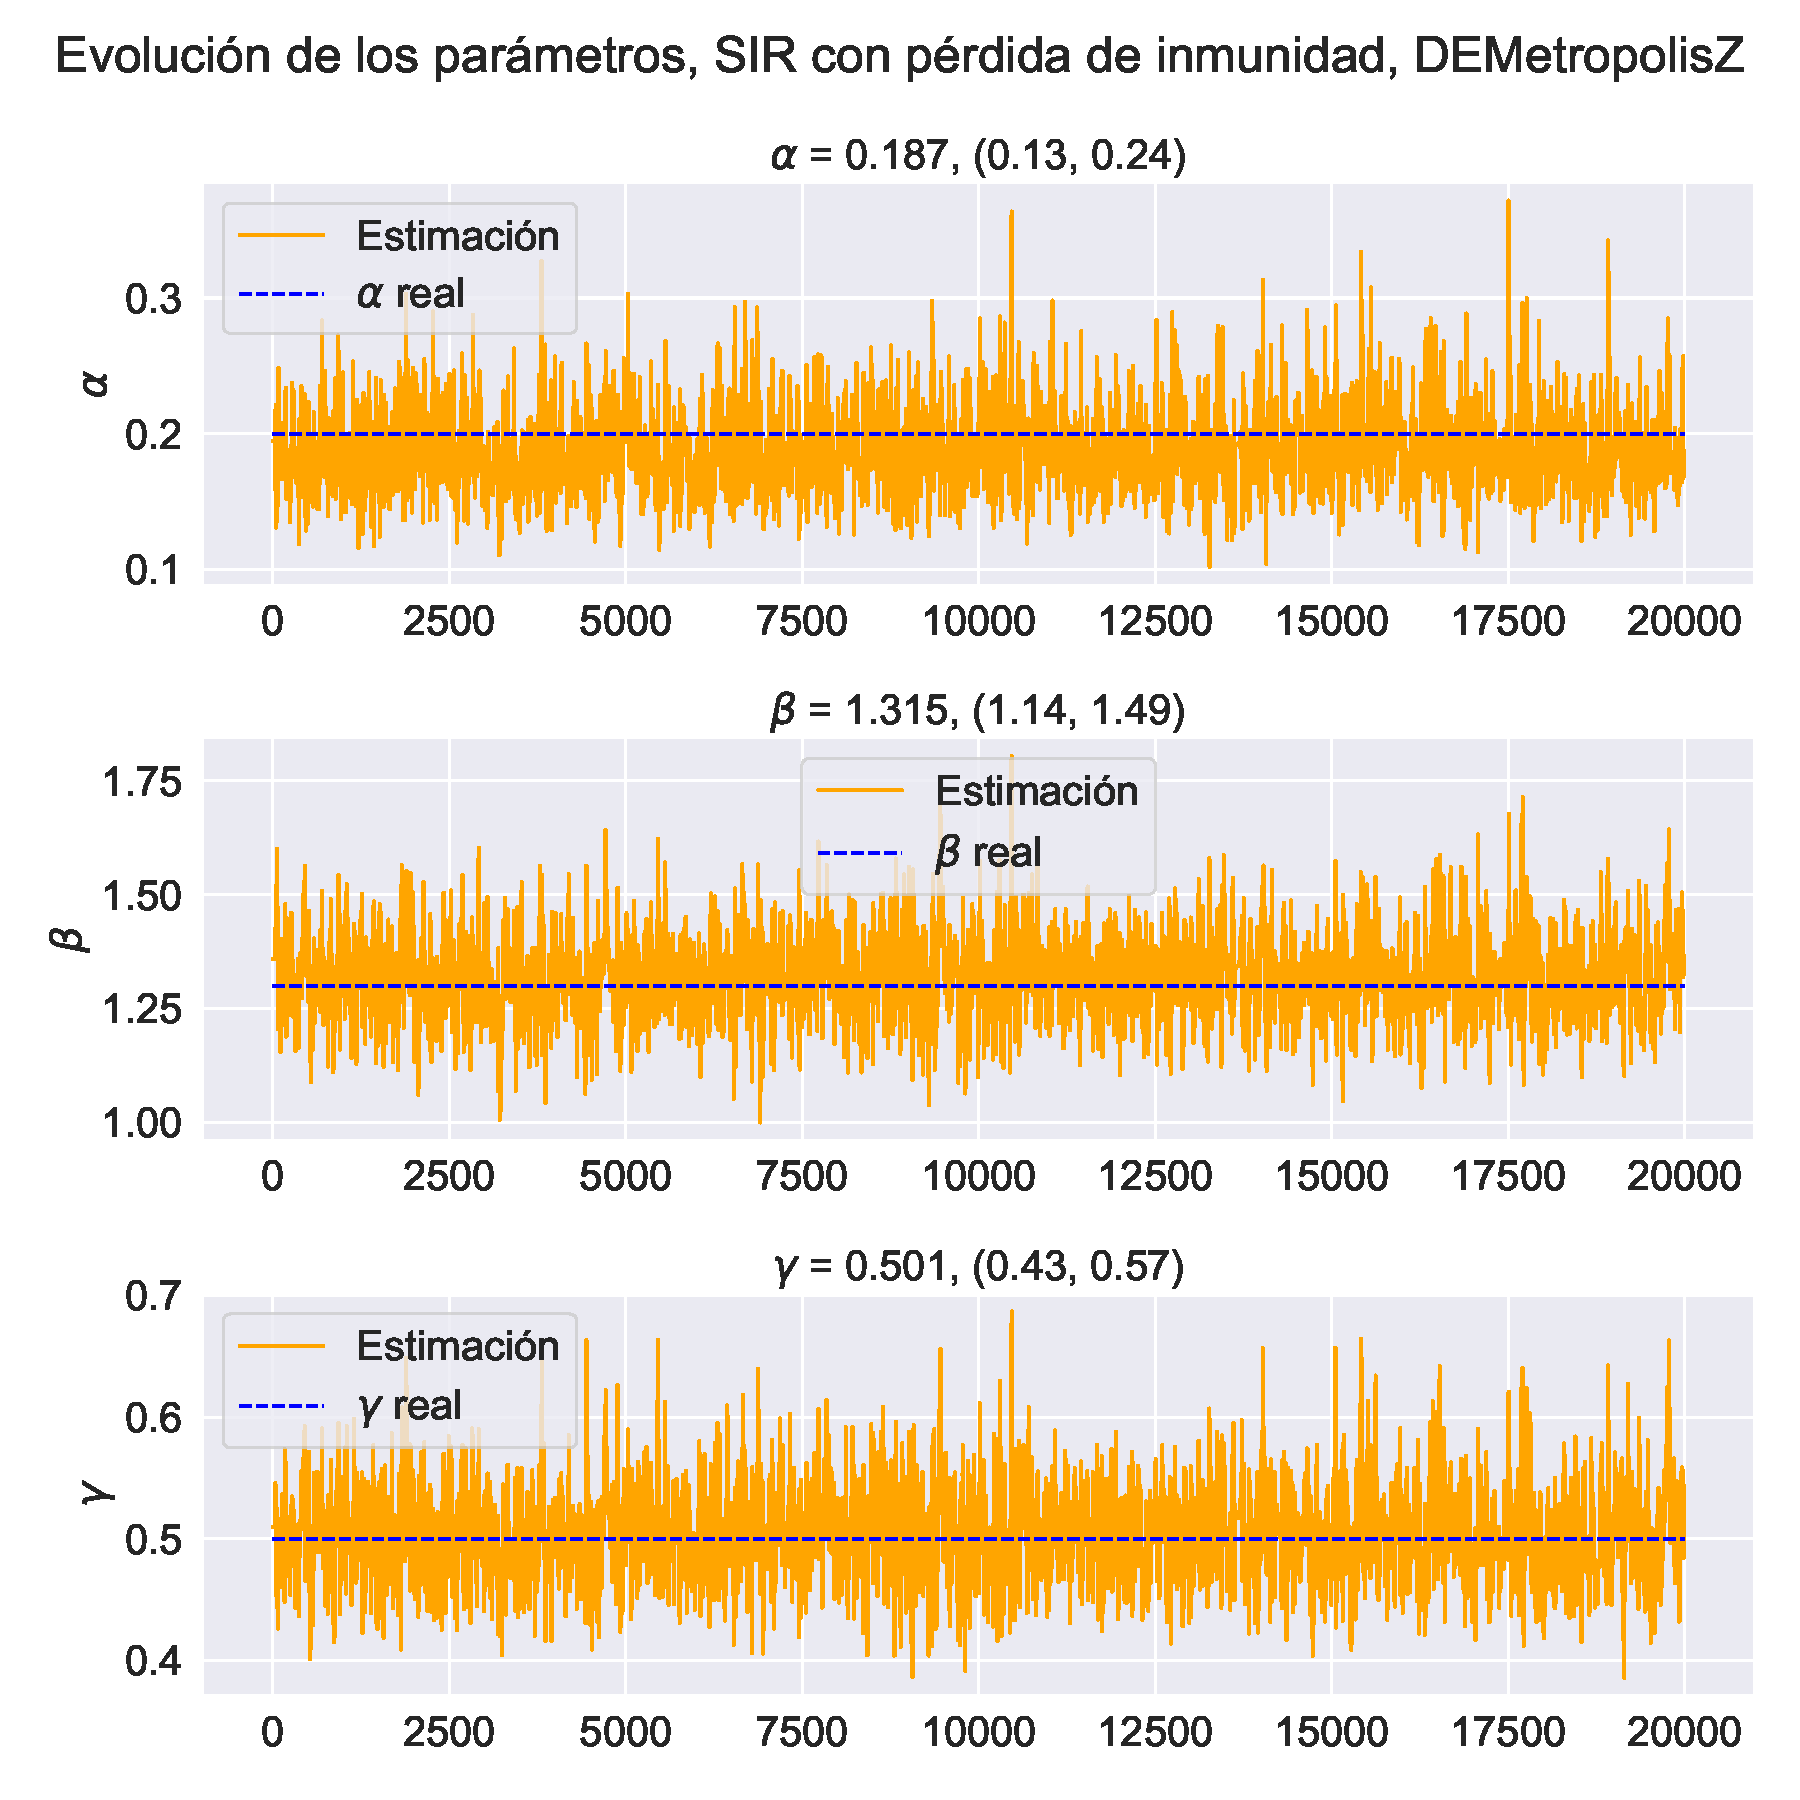
\includegraphics[width=\linewidth]{img/content/chapter4/DEMetropolis_sir_rec_params_trace.pdf}
        \caption{DEMetropolisZ, 20000 iteraciones de estimación y 20000 de \textit{warm up}.}
        \label{fig:NUTS_sir_rec_params_trace}
    \end{subfigure}
    \begin{subfigure}[b]{0.49\linewidth}
        \centering
        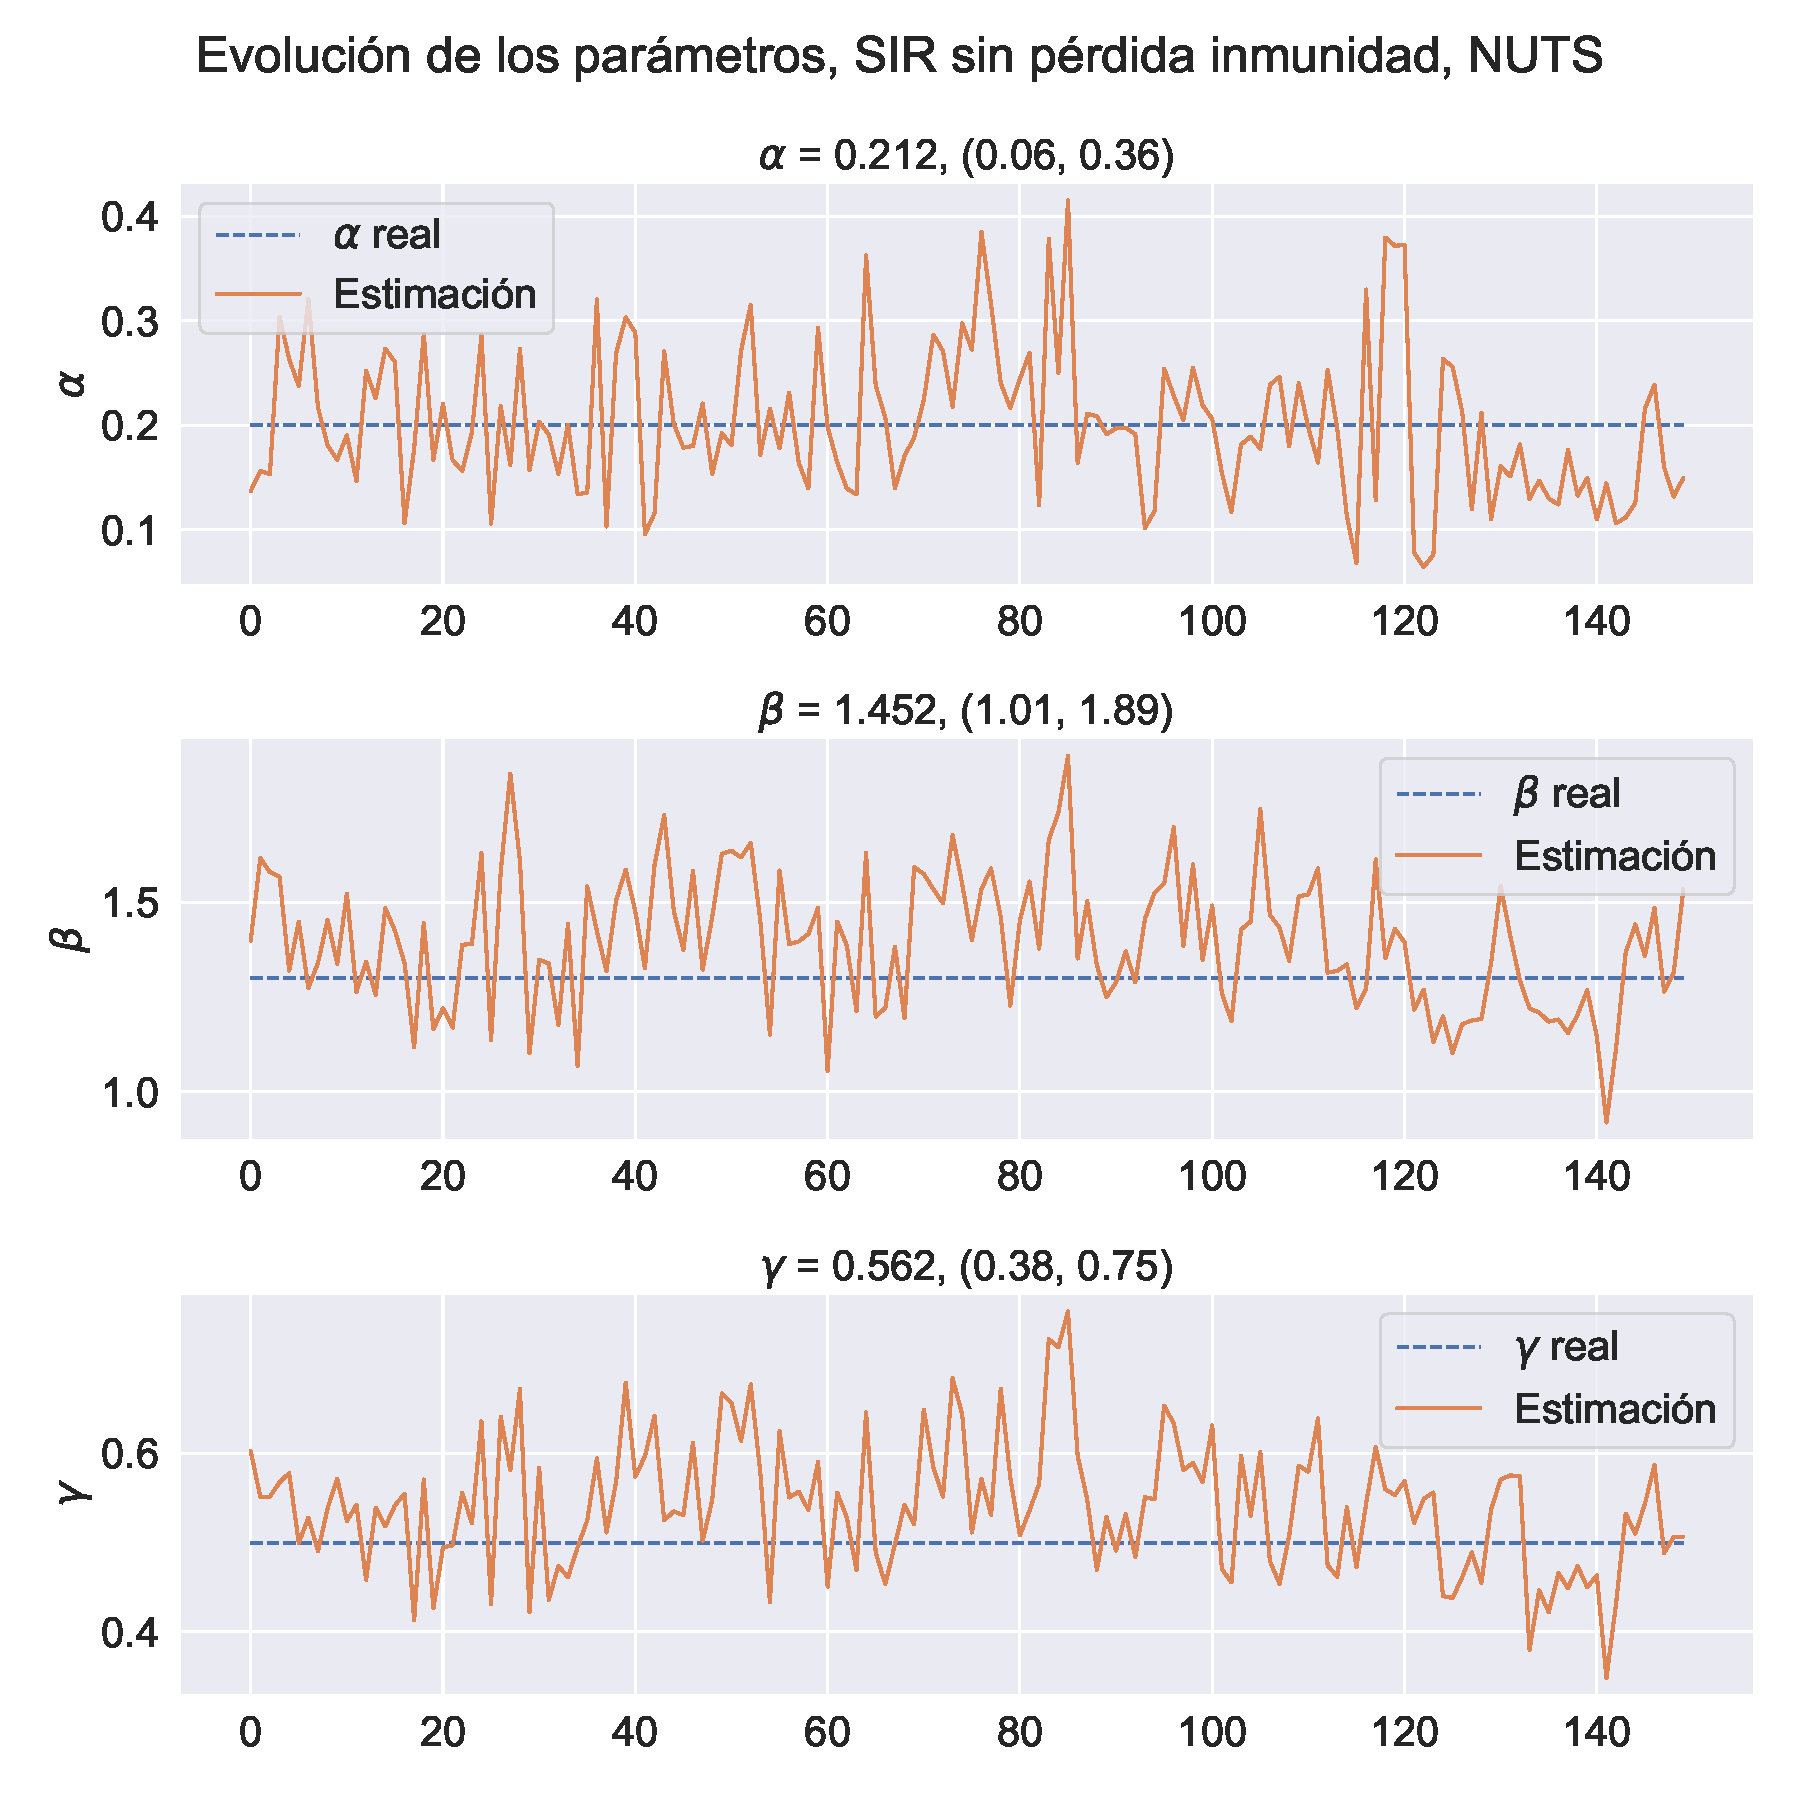
\includegraphics[width=\linewidth]{img/content/chapter4/NUTS_sir_rec_params_trace.pdf}
        \caption{NUTS, 150 iteraciones de estimación y 150 de \textit{warm up}.}
        \label{fig:NUTS_sir_rec_params_trace}
    \end{subfigure}
    \caption{Evolución de los parámetros de SIR con pérdida de inmunidad para una cadena de MCMC. Se muestran las iteraciones posteriores a las de \textit{warm up}, en naranjo el valor estimado del parámetro y en línea punteada el valor real.}
    \label{fig:MCMC_sir_params_trace}
\end{figure}

\begin{figure}[h]
    \centering
    \begin{subfigure}[b]{\linewidth}
        \centering
        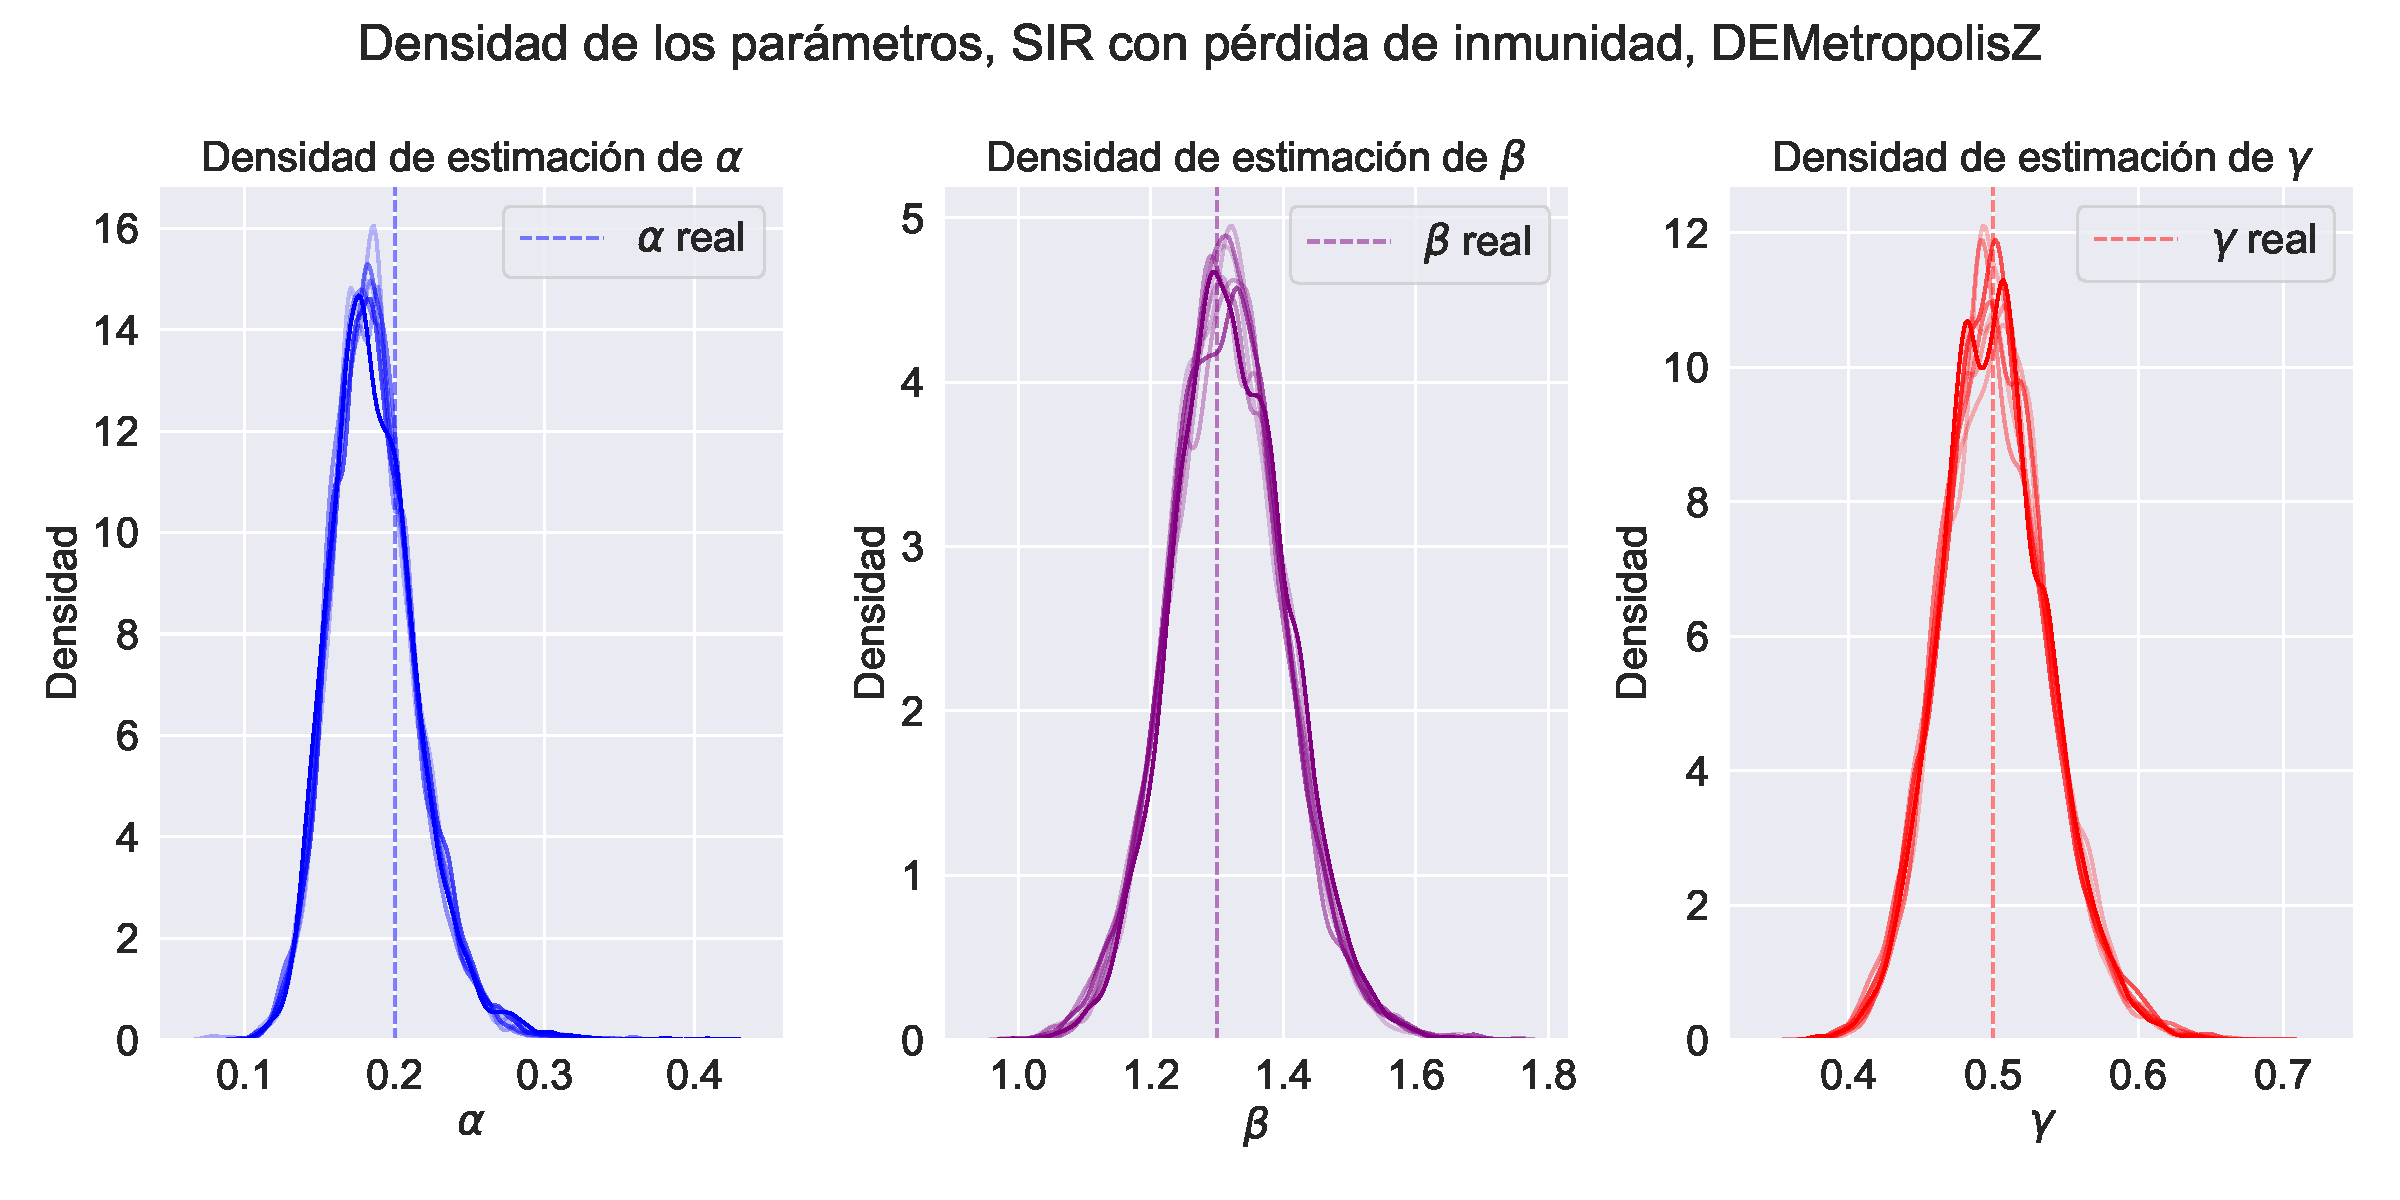
\includegraphics[width=0.55\linewidth]{img/content/chapter4/DEMetropolis_sir_rec_params_density.pdf}
        \caption{Densidad de las 8 cadenas.}
    \end{subfigure}
     \begin{subfigure}[b]{\linewidth}
        \centering
        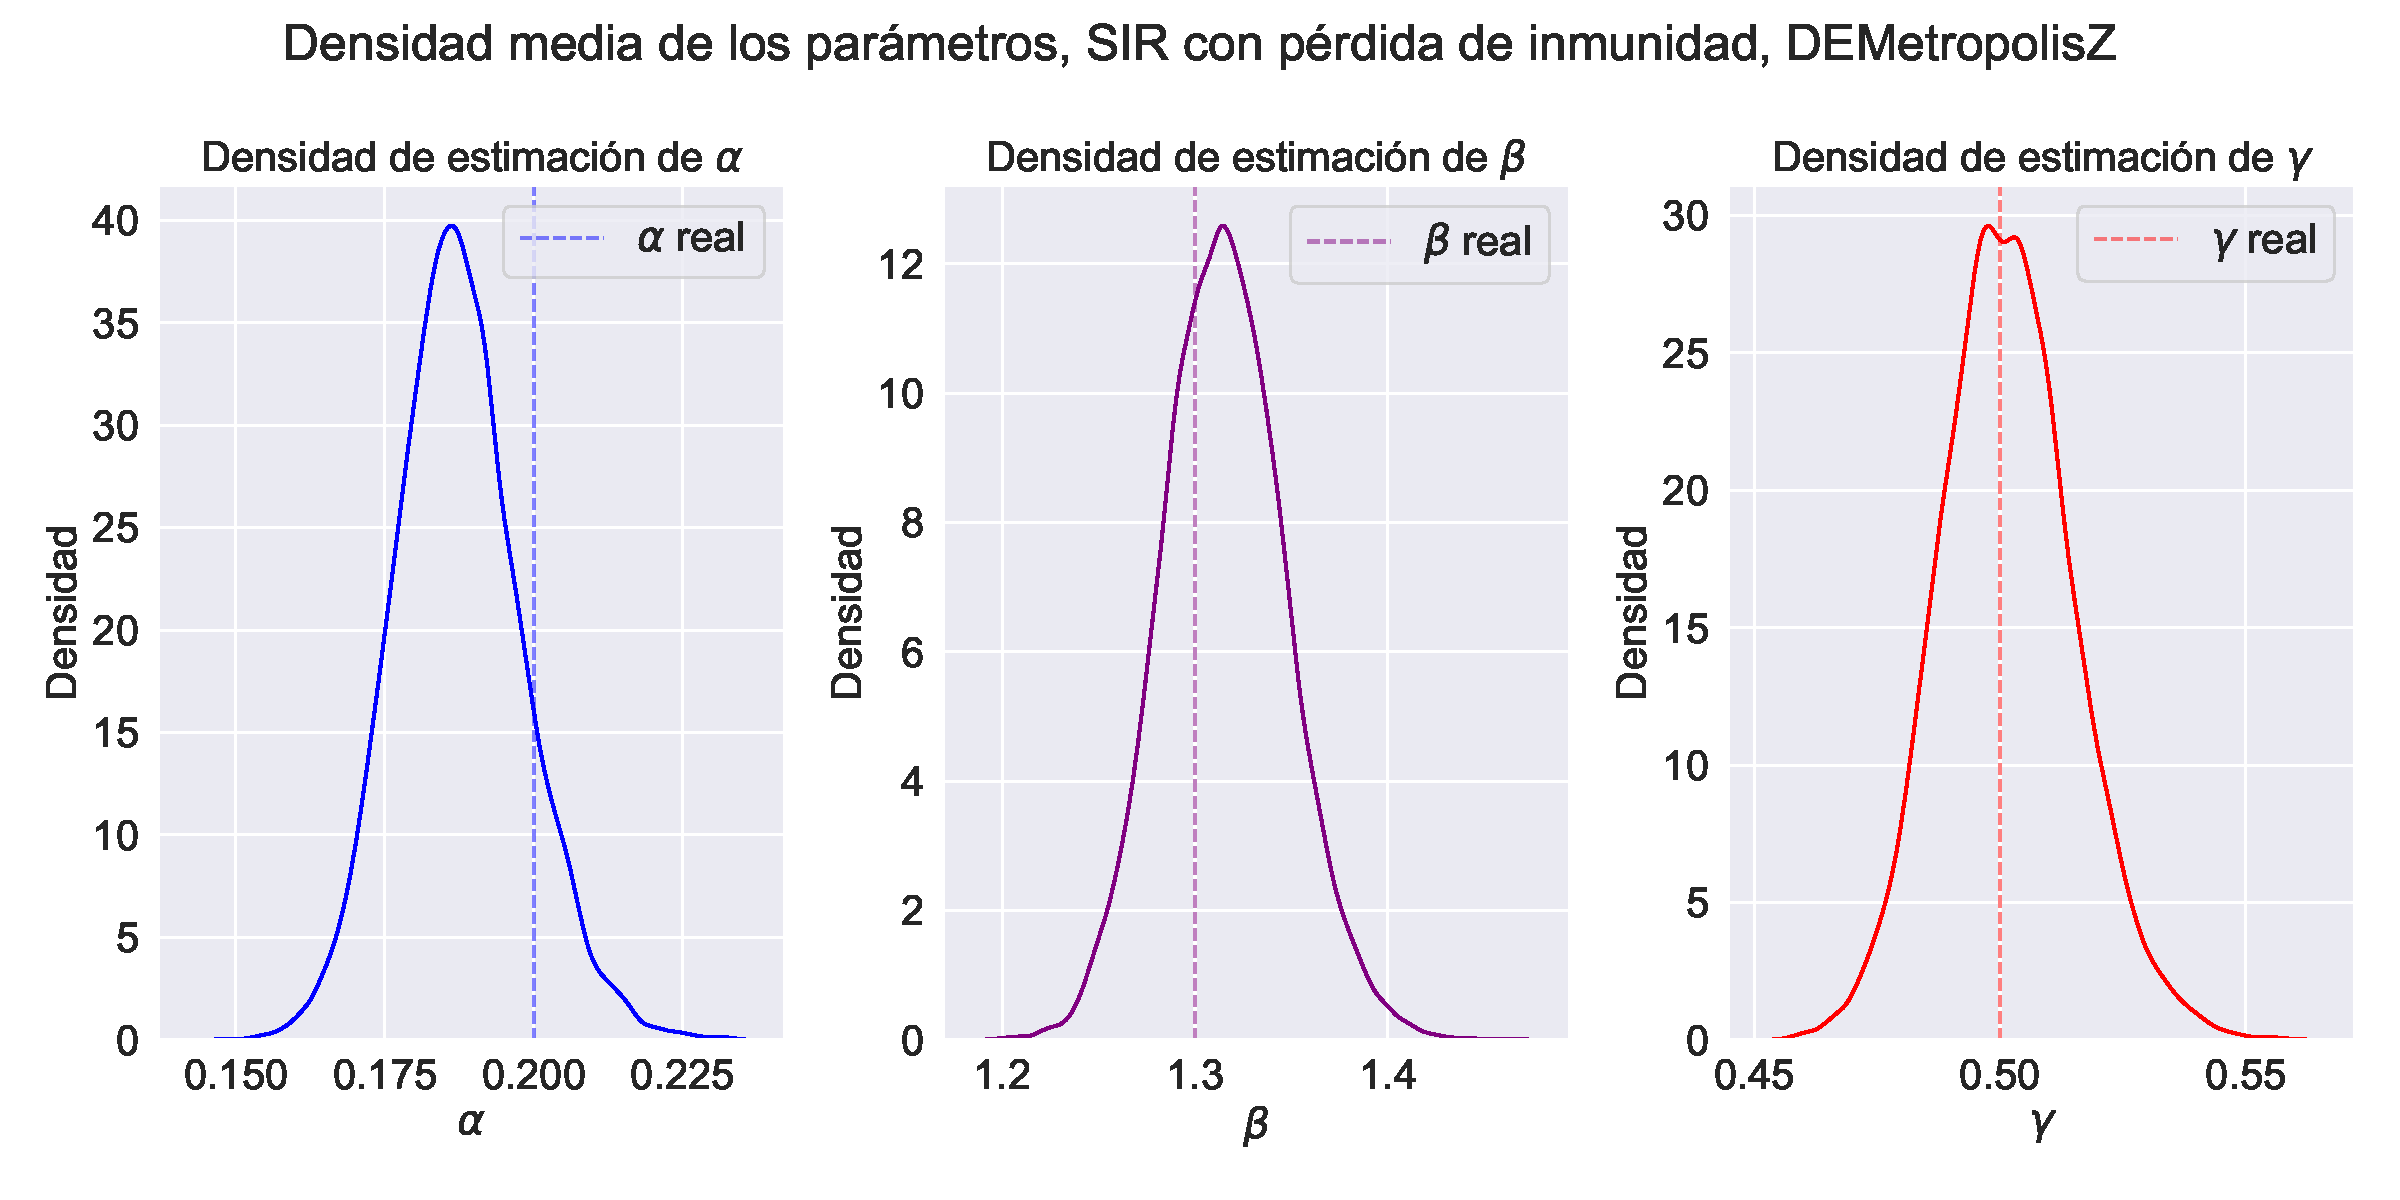
\includegraphics[width=0.55\linewidth]{img/content/chapter4/DEMetropolis_sir_rec_params_density_mean.pdf}
        \caption{Densidad promedio entre las 8 cadenas.}
    \end{subfigure}
    \caption{Densidad de los parámetros del modelo SIR con pérdidad de inmunidad estimados con MCMC con \textit{sampler} DEMetropolisZ.}
\end{figure}

\begin{figure}[h]
    \centering
    \begin{subfigure}[b]{\linewidth}
        \centering
        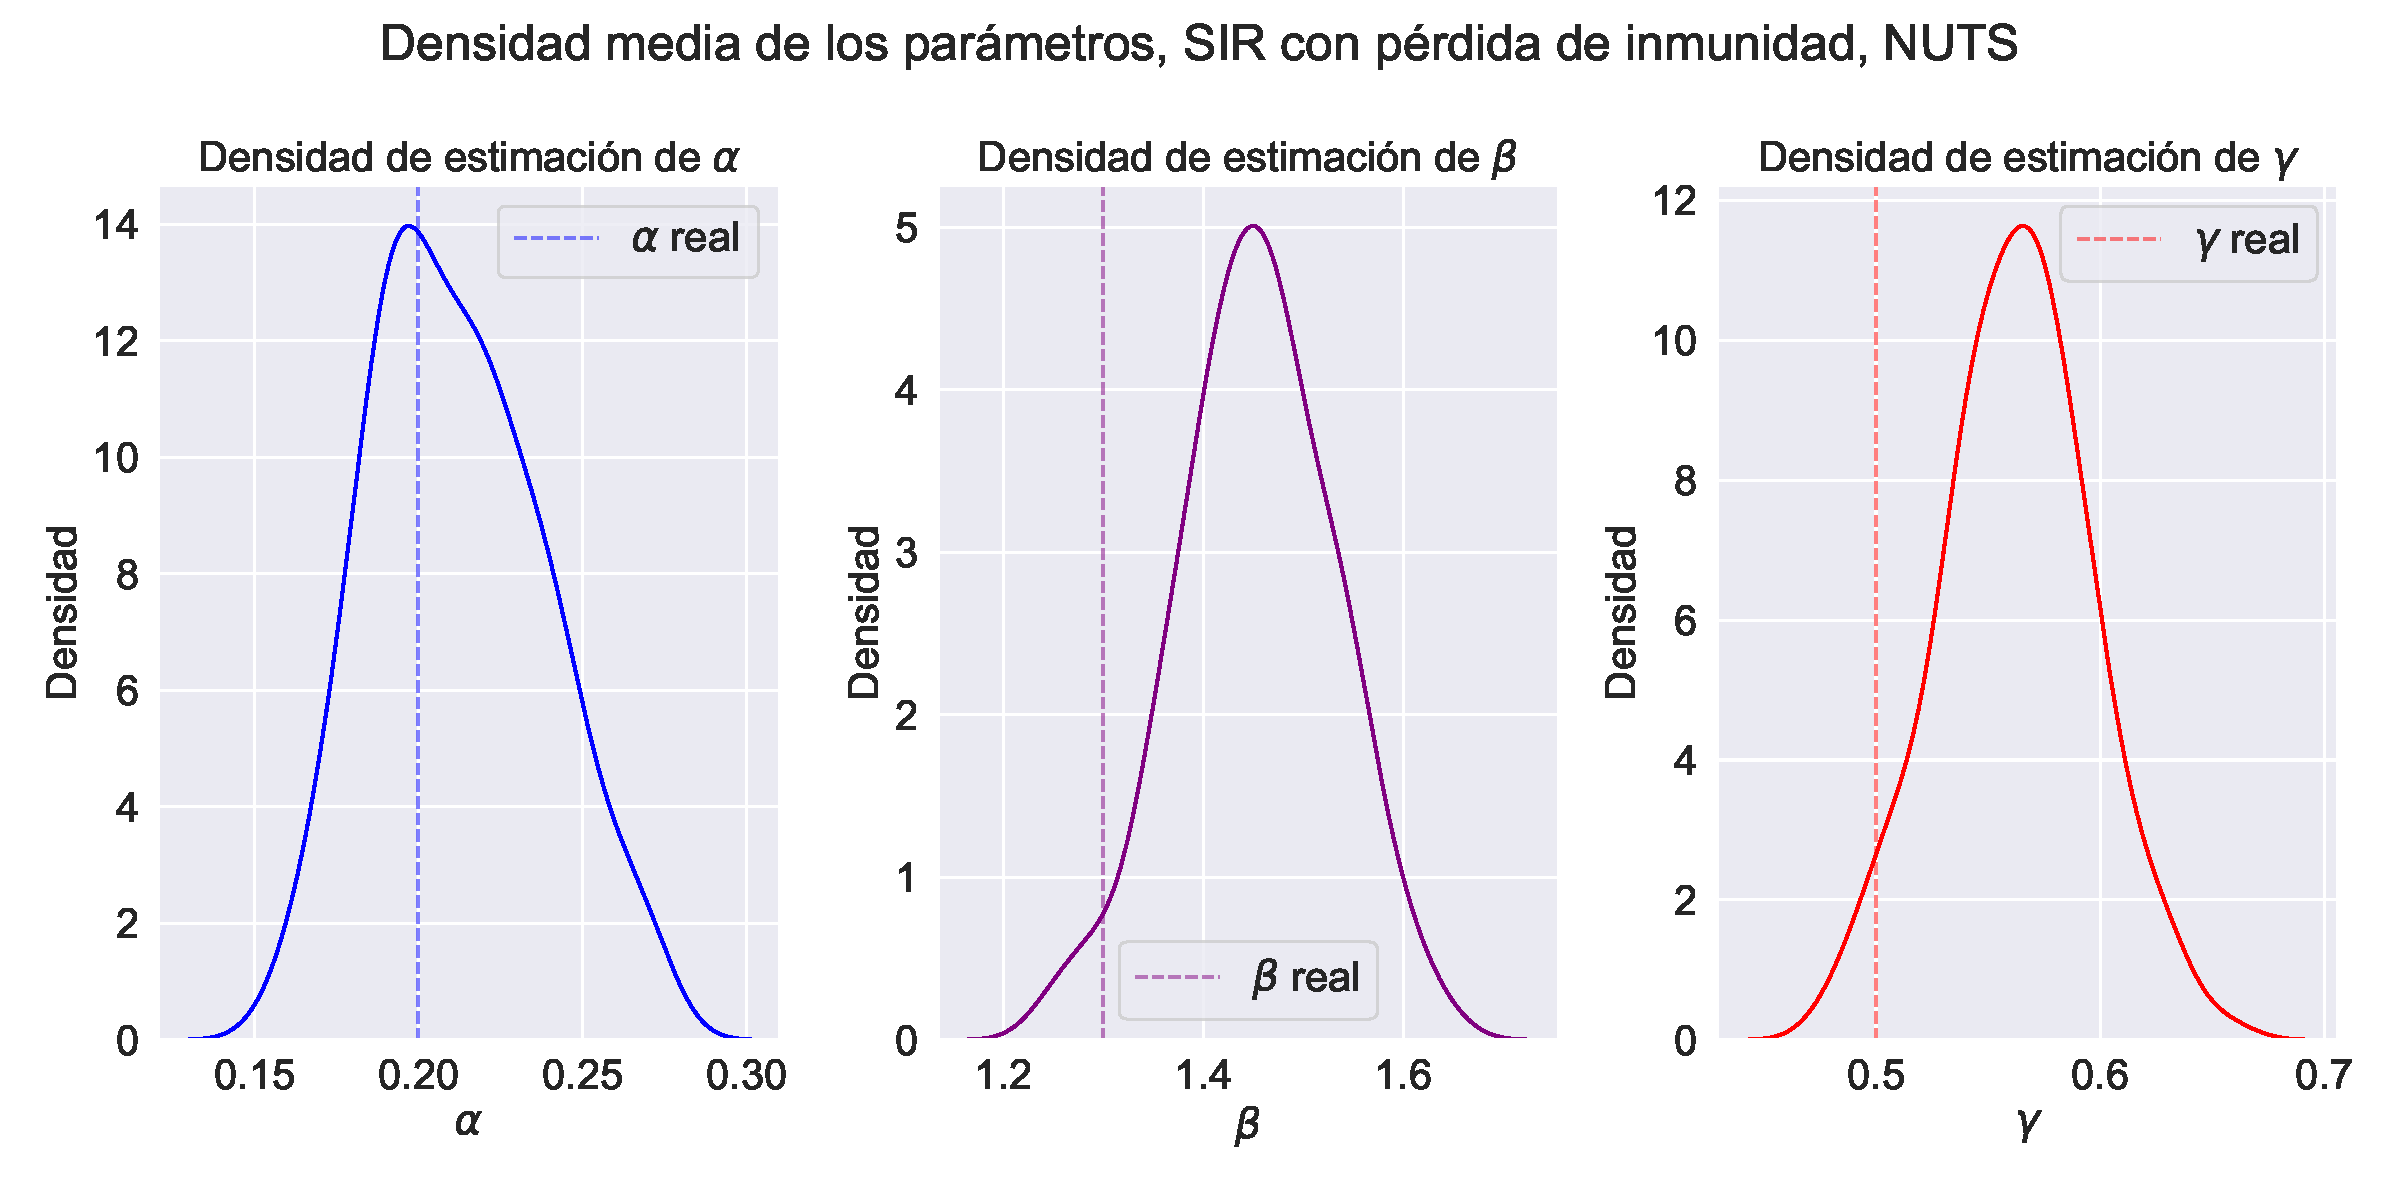
\includegraphics[width=0.55\linewidth]{img/content/chapter4/NUTS_sir_rec_params_density.pdf}
        \caption{Densidad de las 8 cadenas.}
    \end{subfigure}
     \begin{subfigure}[b]{\linewidth}
        \centering
        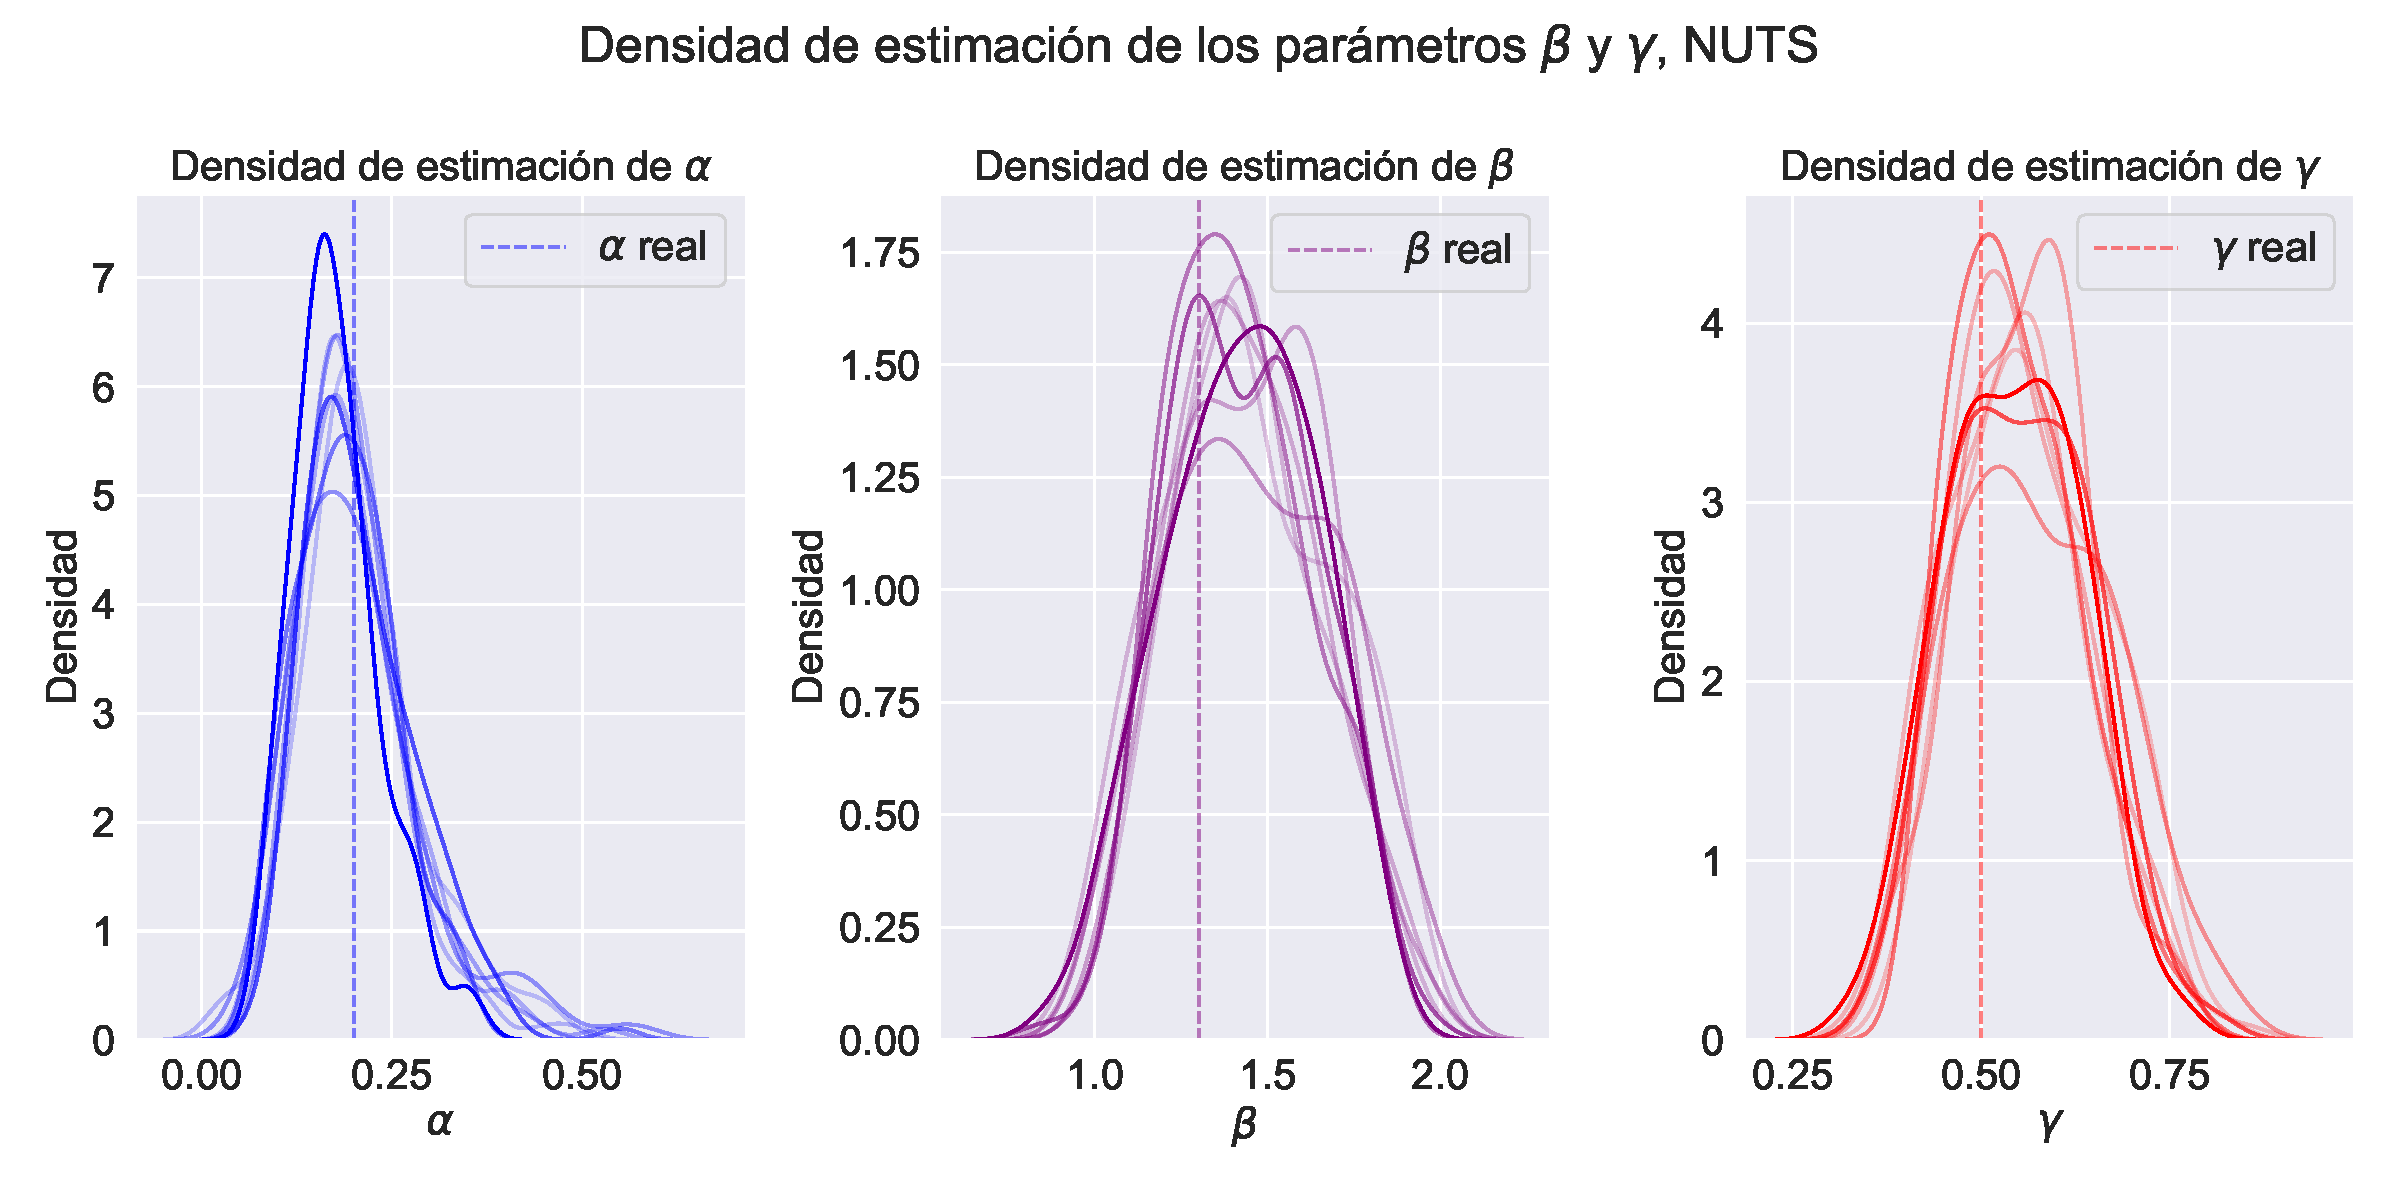
\includegraphics[width=0.55\linewidth]{img/content/chapter4/NUTS_sir_rec_params_density_mean.pdf}
        \caption{Densidad promedio entre las 8 cadenas.}
    \end{subfigure}
    \caption{Densidad de los parámetros del modelo SIR con pérdida de inmunidad estimados con MCMC con \textit{sampler} NUTS.}
\end{figure}

\begin{figure}[h]
    \centering
    \begin{subfigure}[b]{0.49\linewidth}
        \centering
        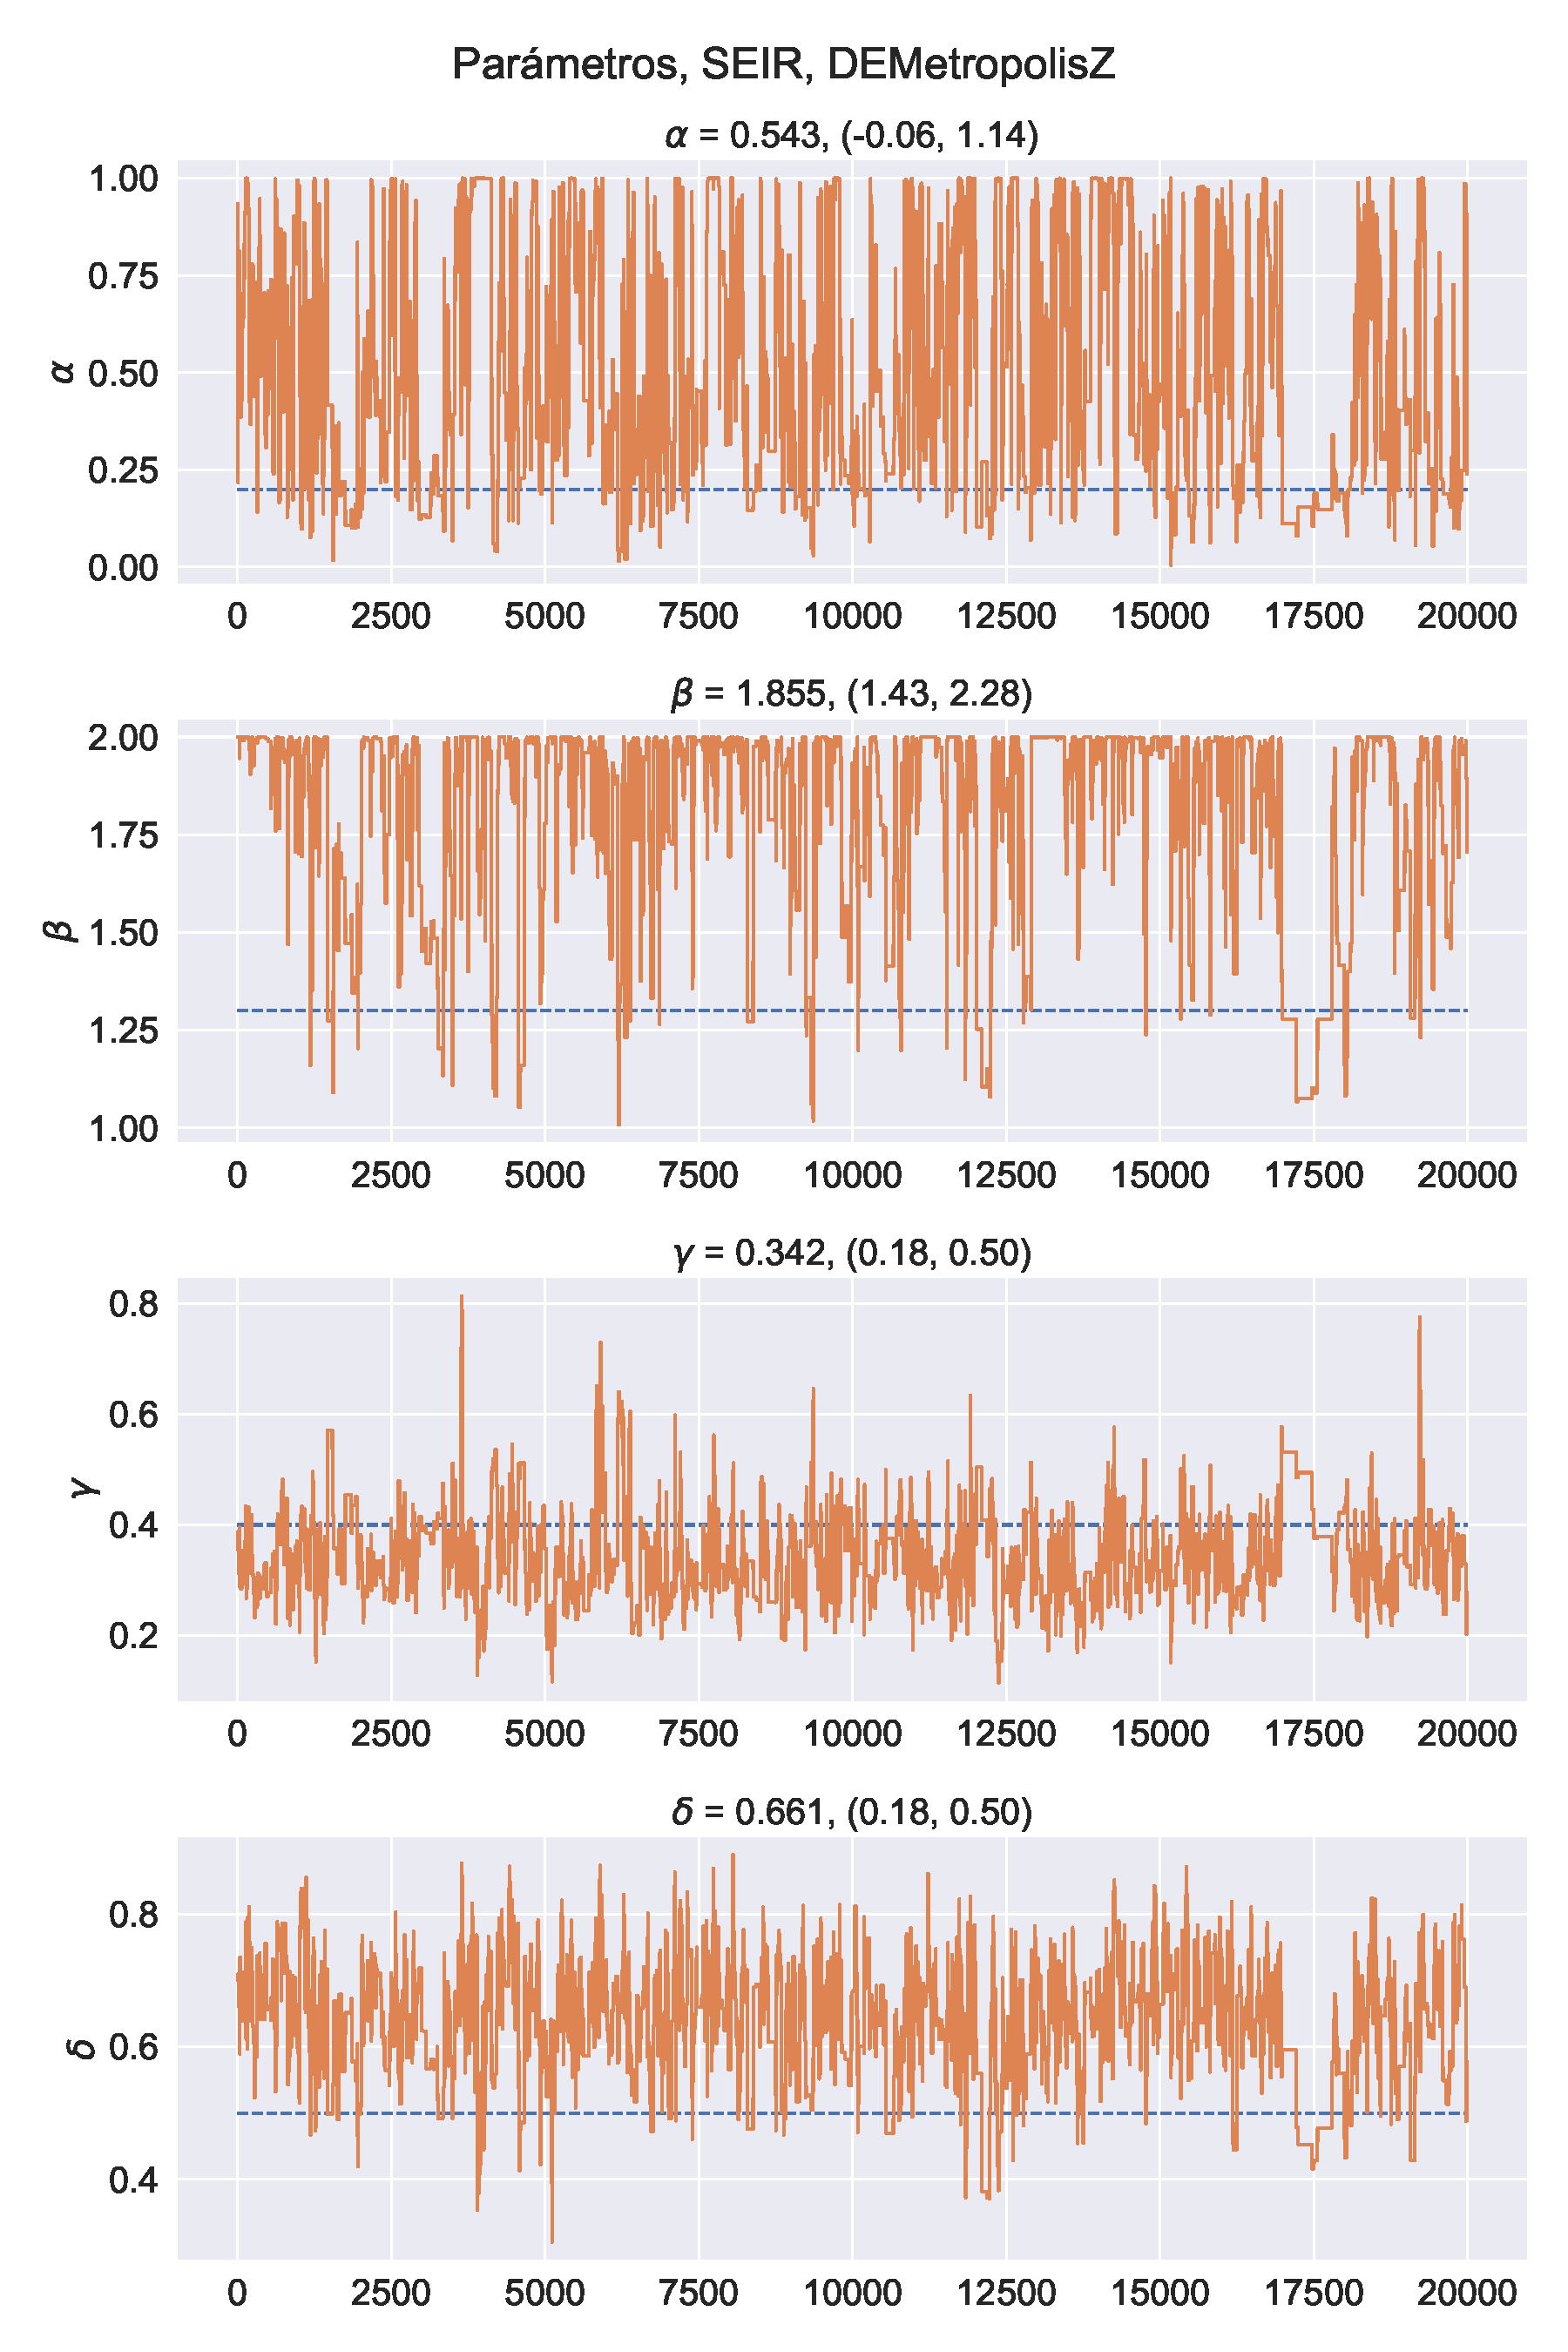
\includegraphics[width=\linewidth]{img/content/chapter4/DEMetropolis_seir_params_trace.pdf}
        \caption{DEMetropolisZ, 20000 iteraciones de estimación y 20000 de \textit{warm up}.}
        \label{fig:NUTS_seir_params_trace}
    \end{subfigure}
    \begin{subfigure}[b]{0.49\linewidth}
        \centering
        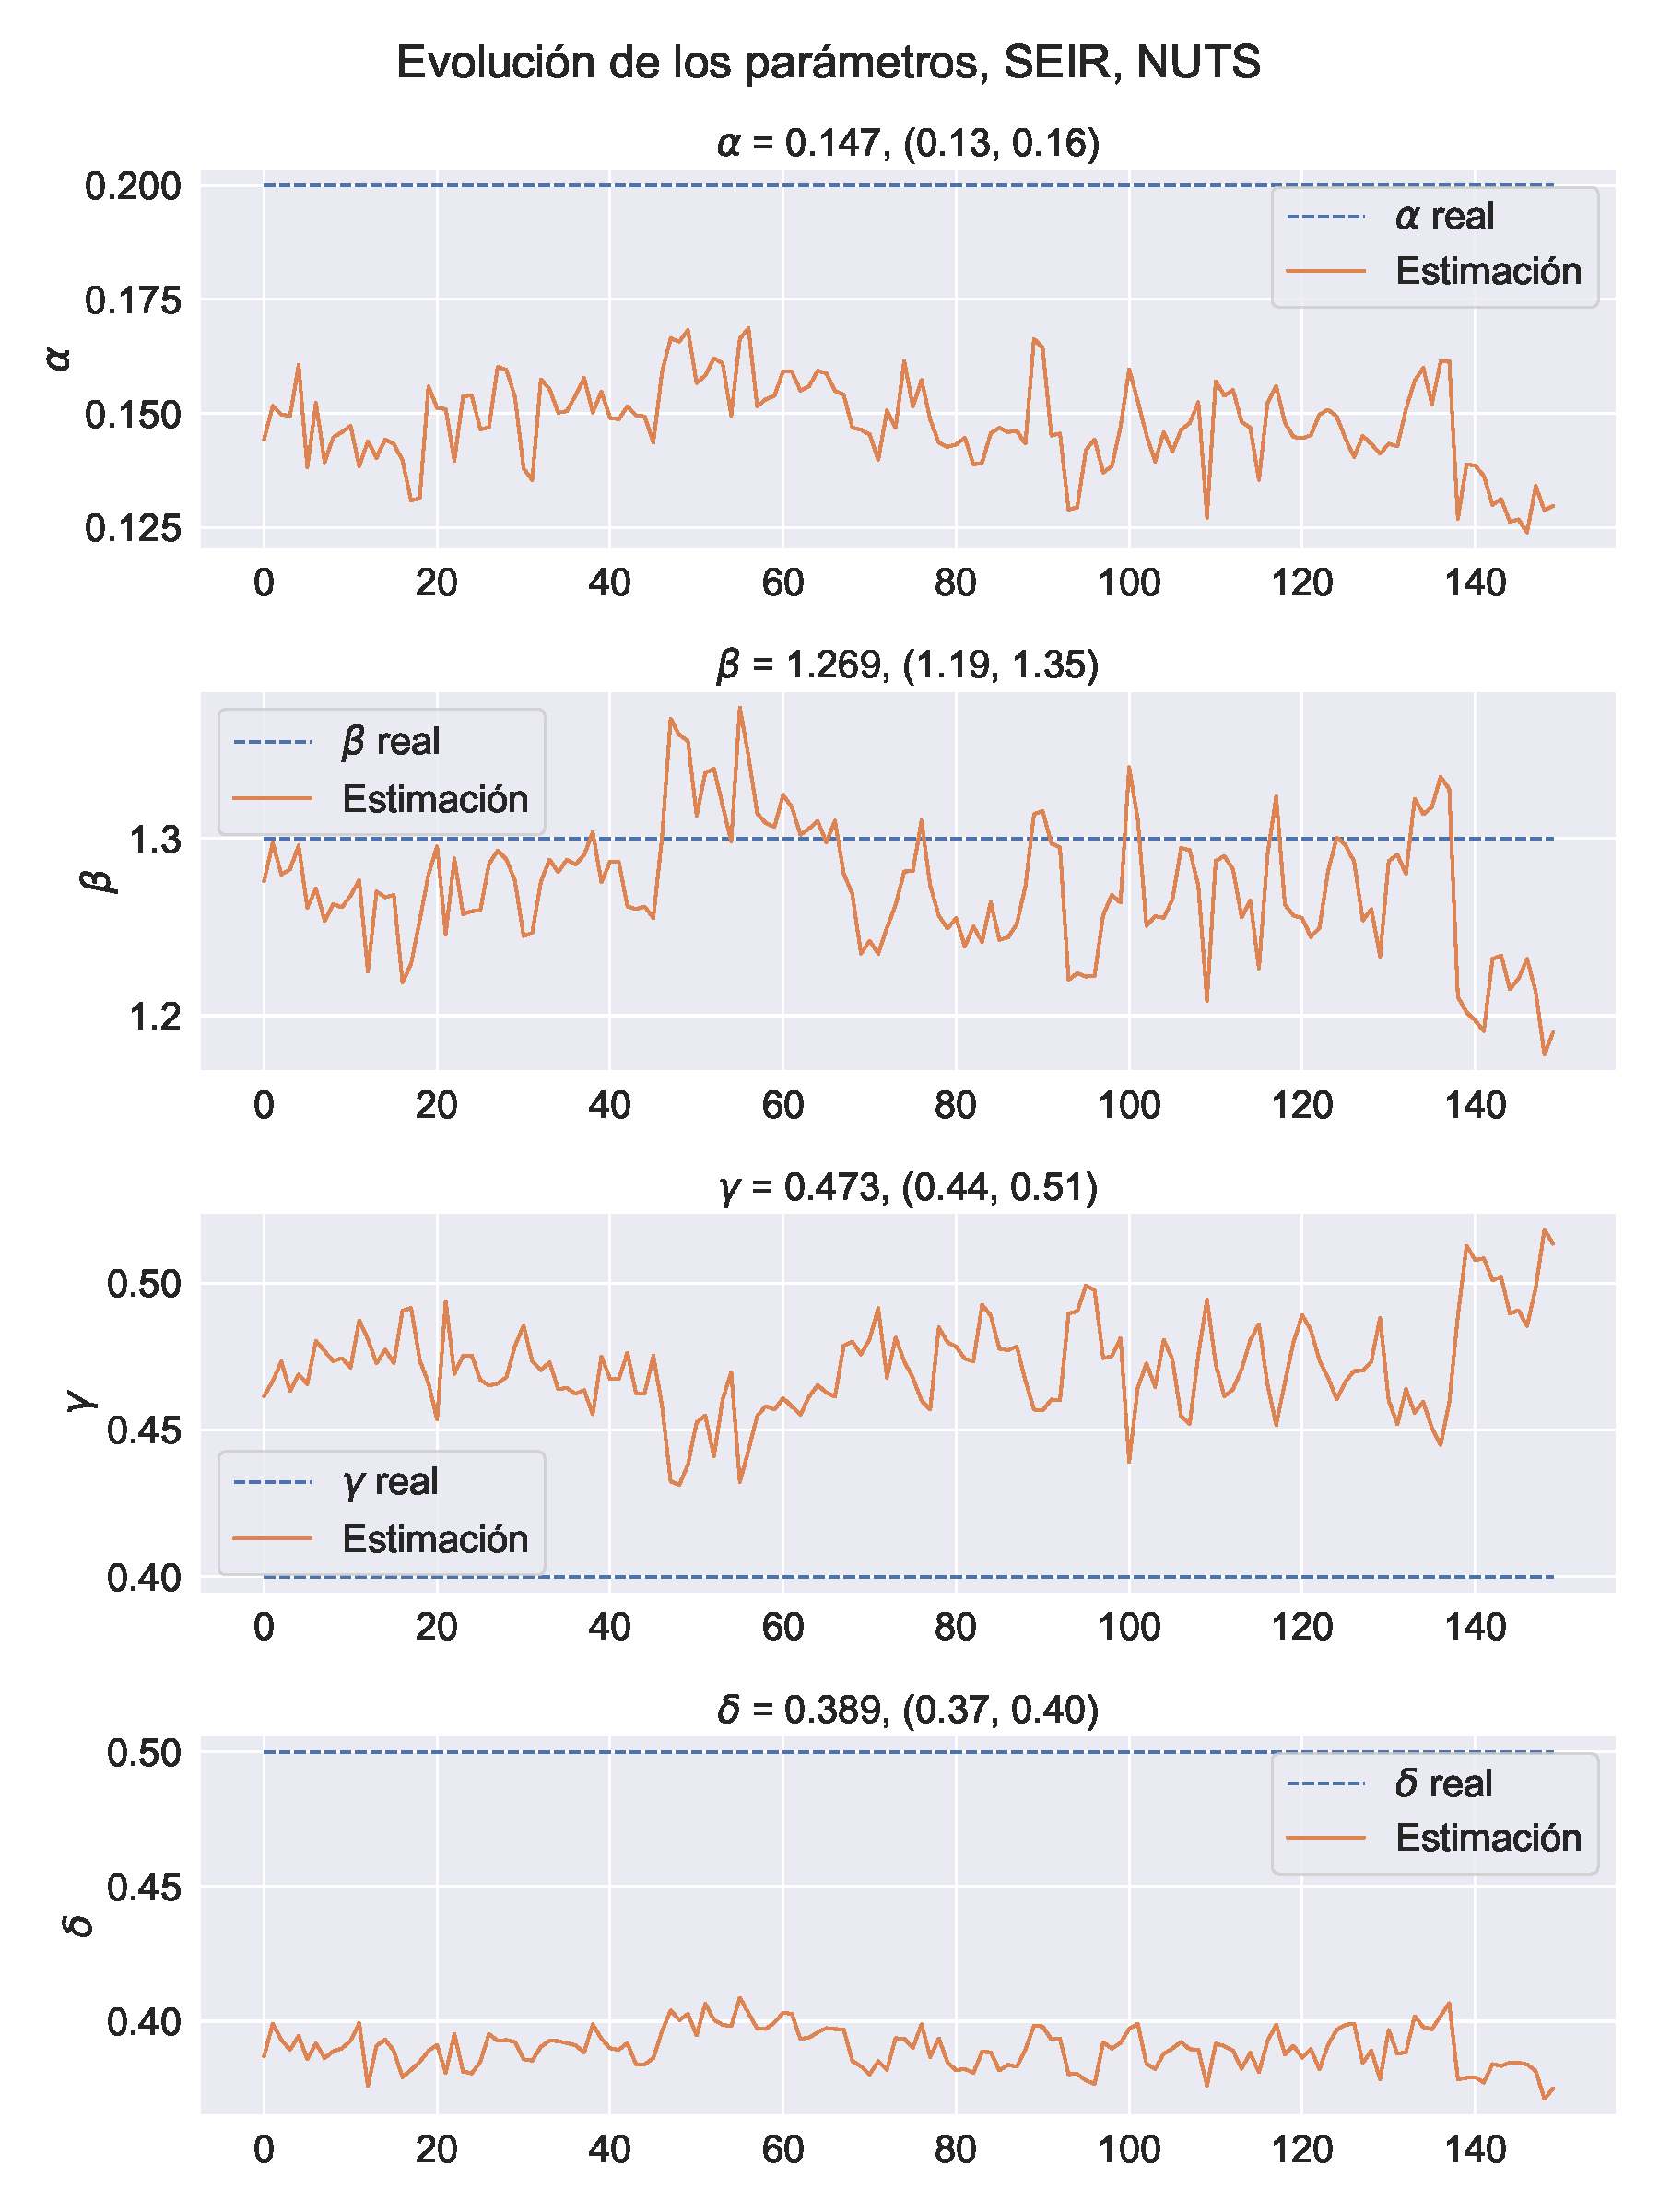
\includegraphics[width=\linewidth]{img/content/chapter4/NUTS_seir_params_trace.pdf}
        \caption{NUTS, 150 iteraciones de estimación y 150 de \textit{warm up}.}
        \label{fig:NUTS_seir_params_trace}
    \end{subfigure}
    \caption{Evolución de los parámetros de SEIR para una cadena de MCMC. Se muestran las iteraciones posteriores a las de \textit{warm up}, en naranjo el valor estimado del parámetro y en línea punteada el valor real.}
    \label{fig:MCMC_seir_params_trace}
\end{figure}

\begin{figure}[h]
    \centering
    \begin{subfigure}[b]{\linewidth}
        \centering
        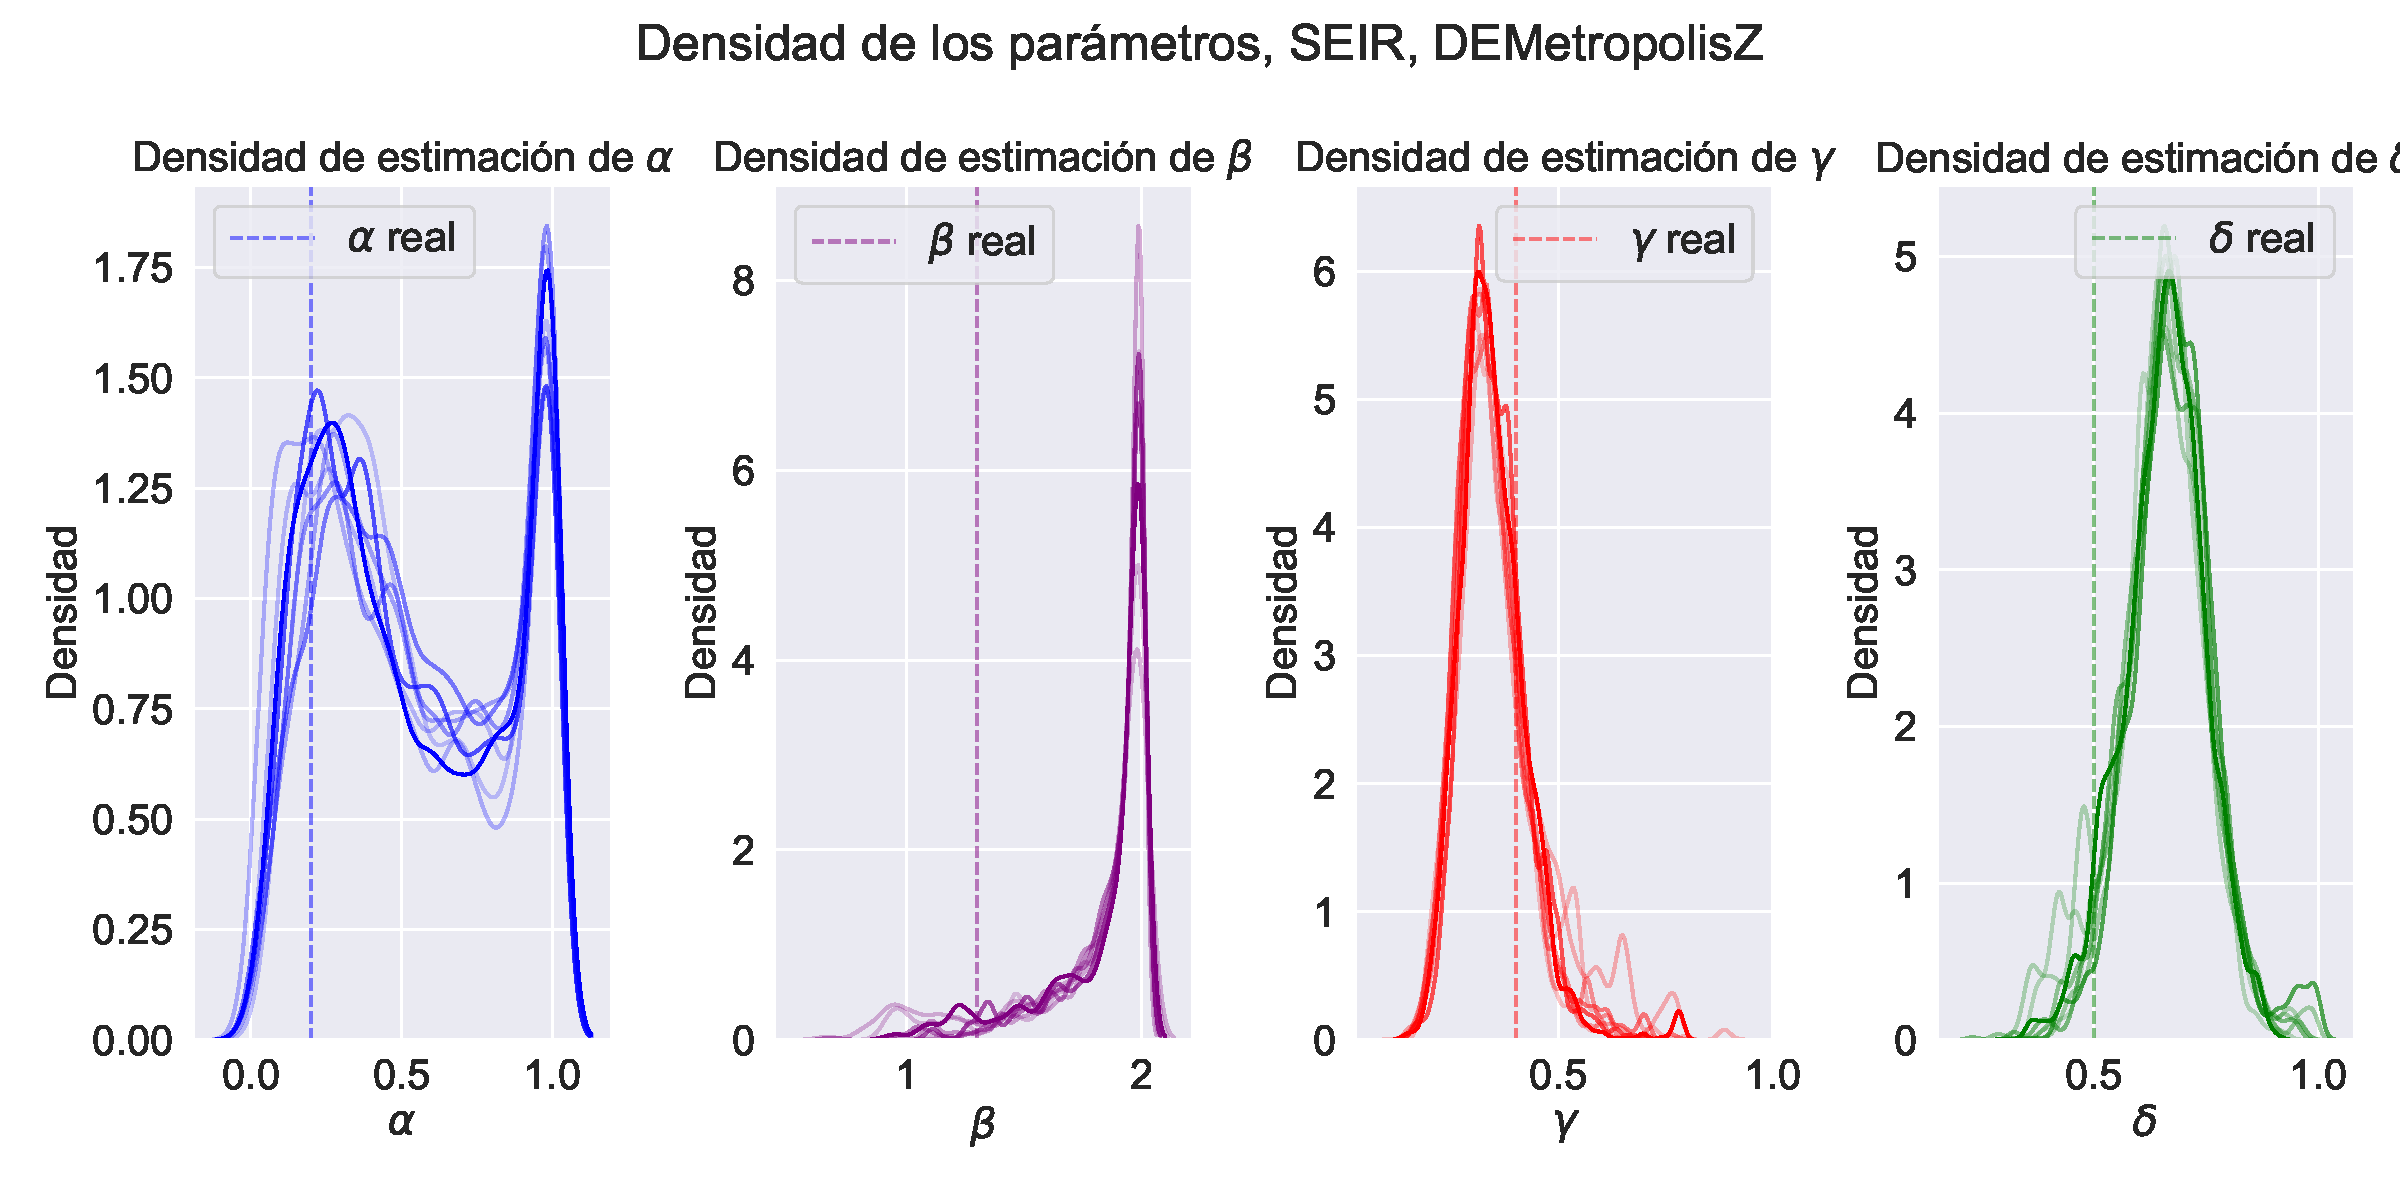
\includegraphics[width=0.55\linewidth]{img/content/chapter4/DEMetropolis_seir_params_density.pdf}
        \caption{Densidad de las 8 cadenas.}
    \end{subfigure}
     \begin{subfigure}[b]{\linewidth}
        \centering
        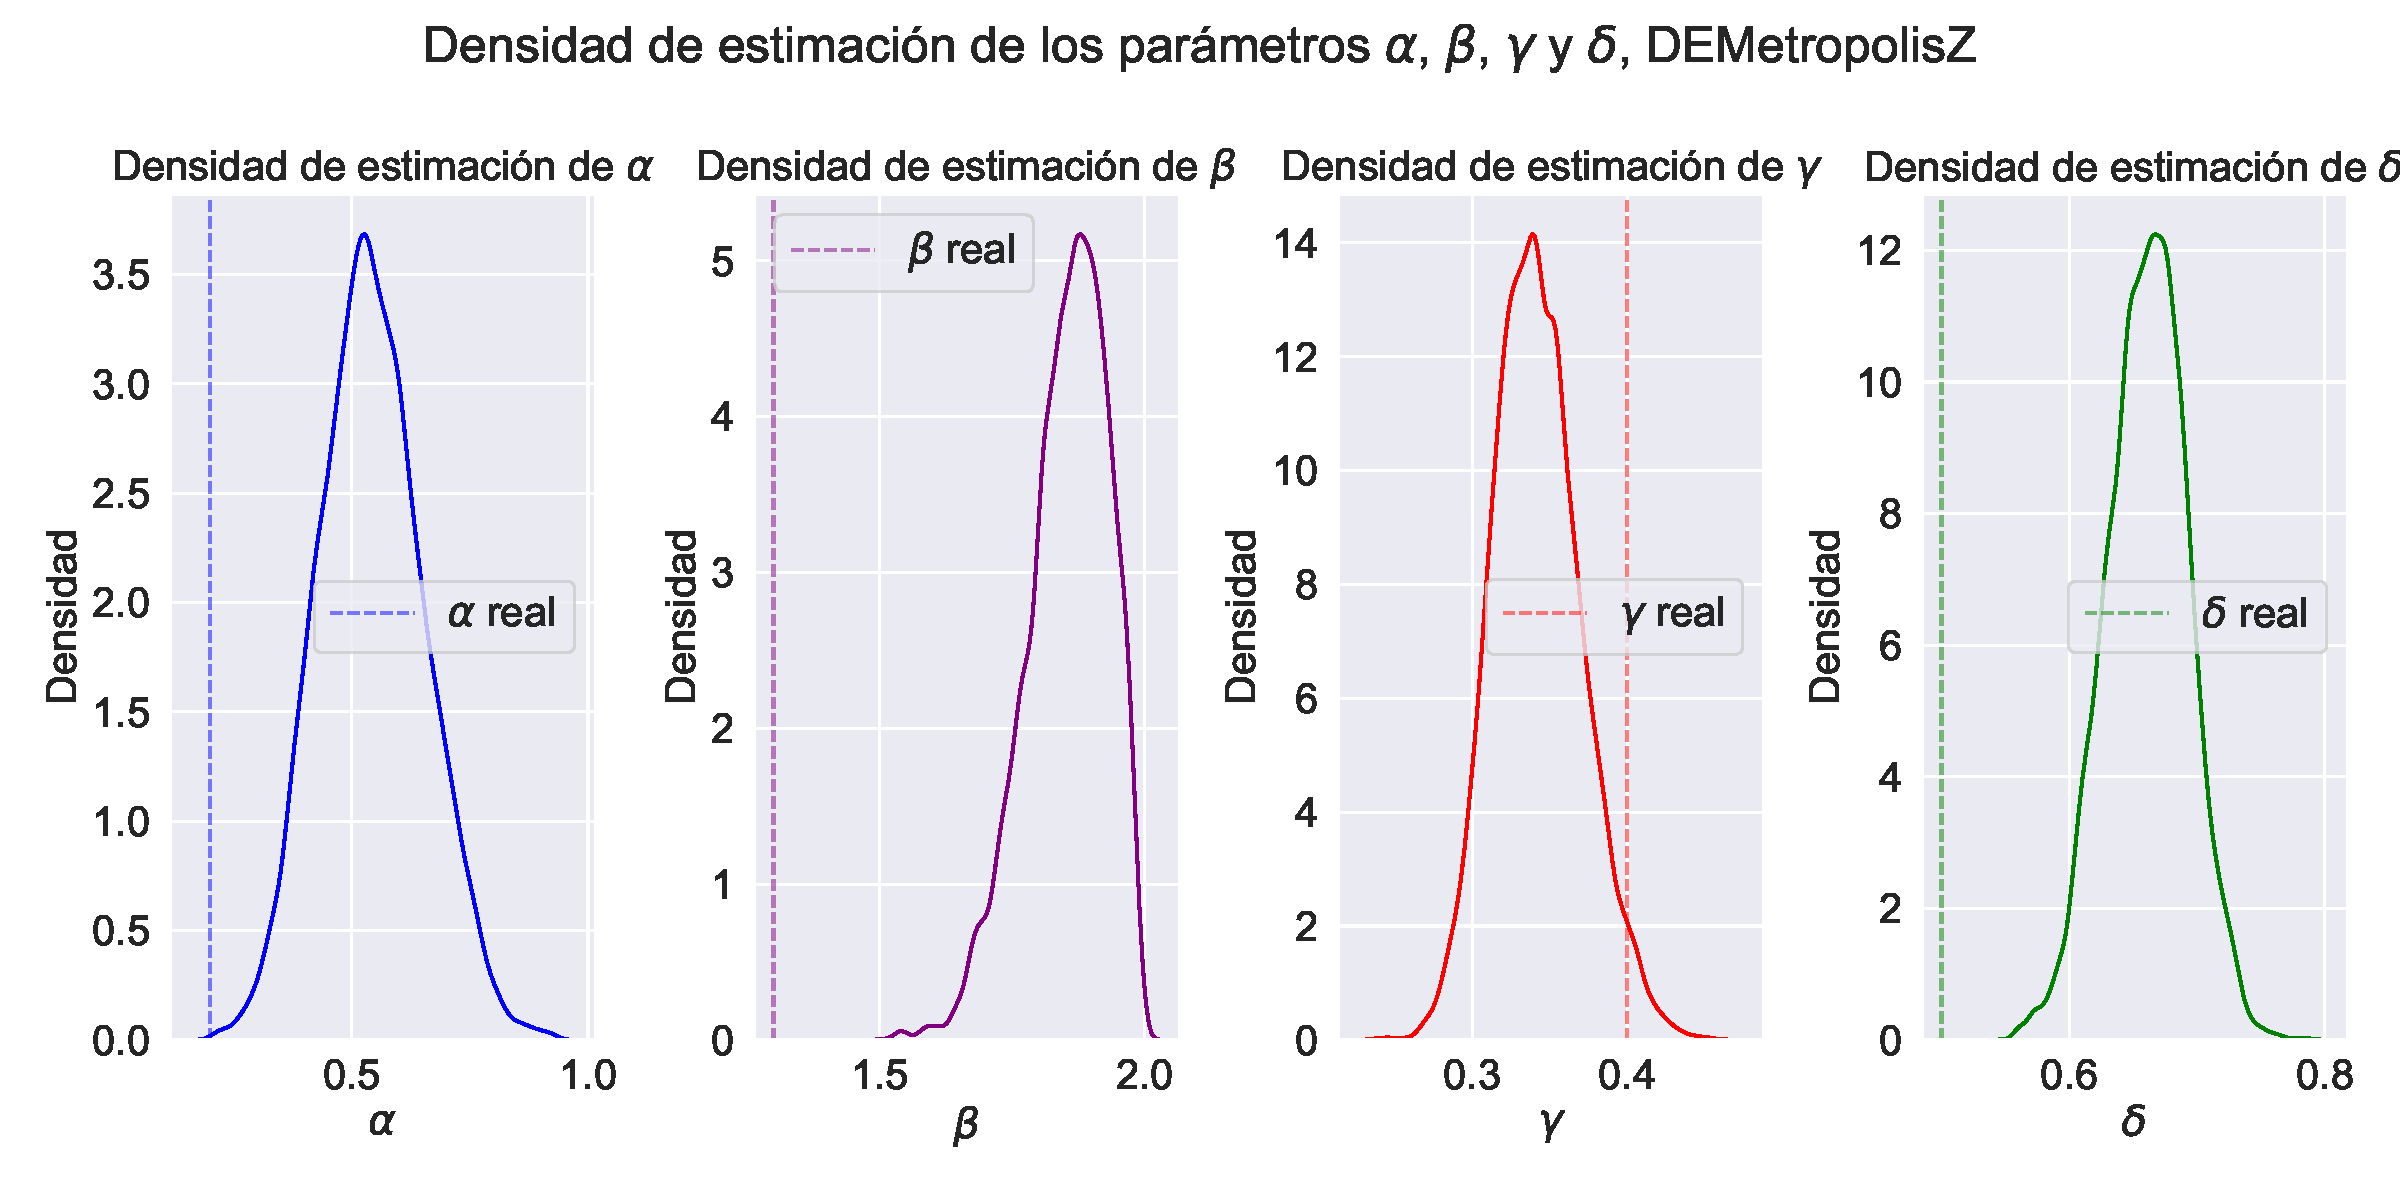
\includegraphics[width=0.55\linewidth]{img/content/chapter4/DEMetropolis_seir_params_density_mean.pdf}
        \caption{Densidad promedio entre las 8 cadenas.}
    \end{subfigure}
    \caption{Densidad de los parámetros del modelo SEIR estimados con MCMC con \textit{sampler} DEMEtropolisZ.}
\end{figure}

\begin{figure}[h]
    \centering
    \begin{subfigure}[b]{\linewidth}
        \centering
        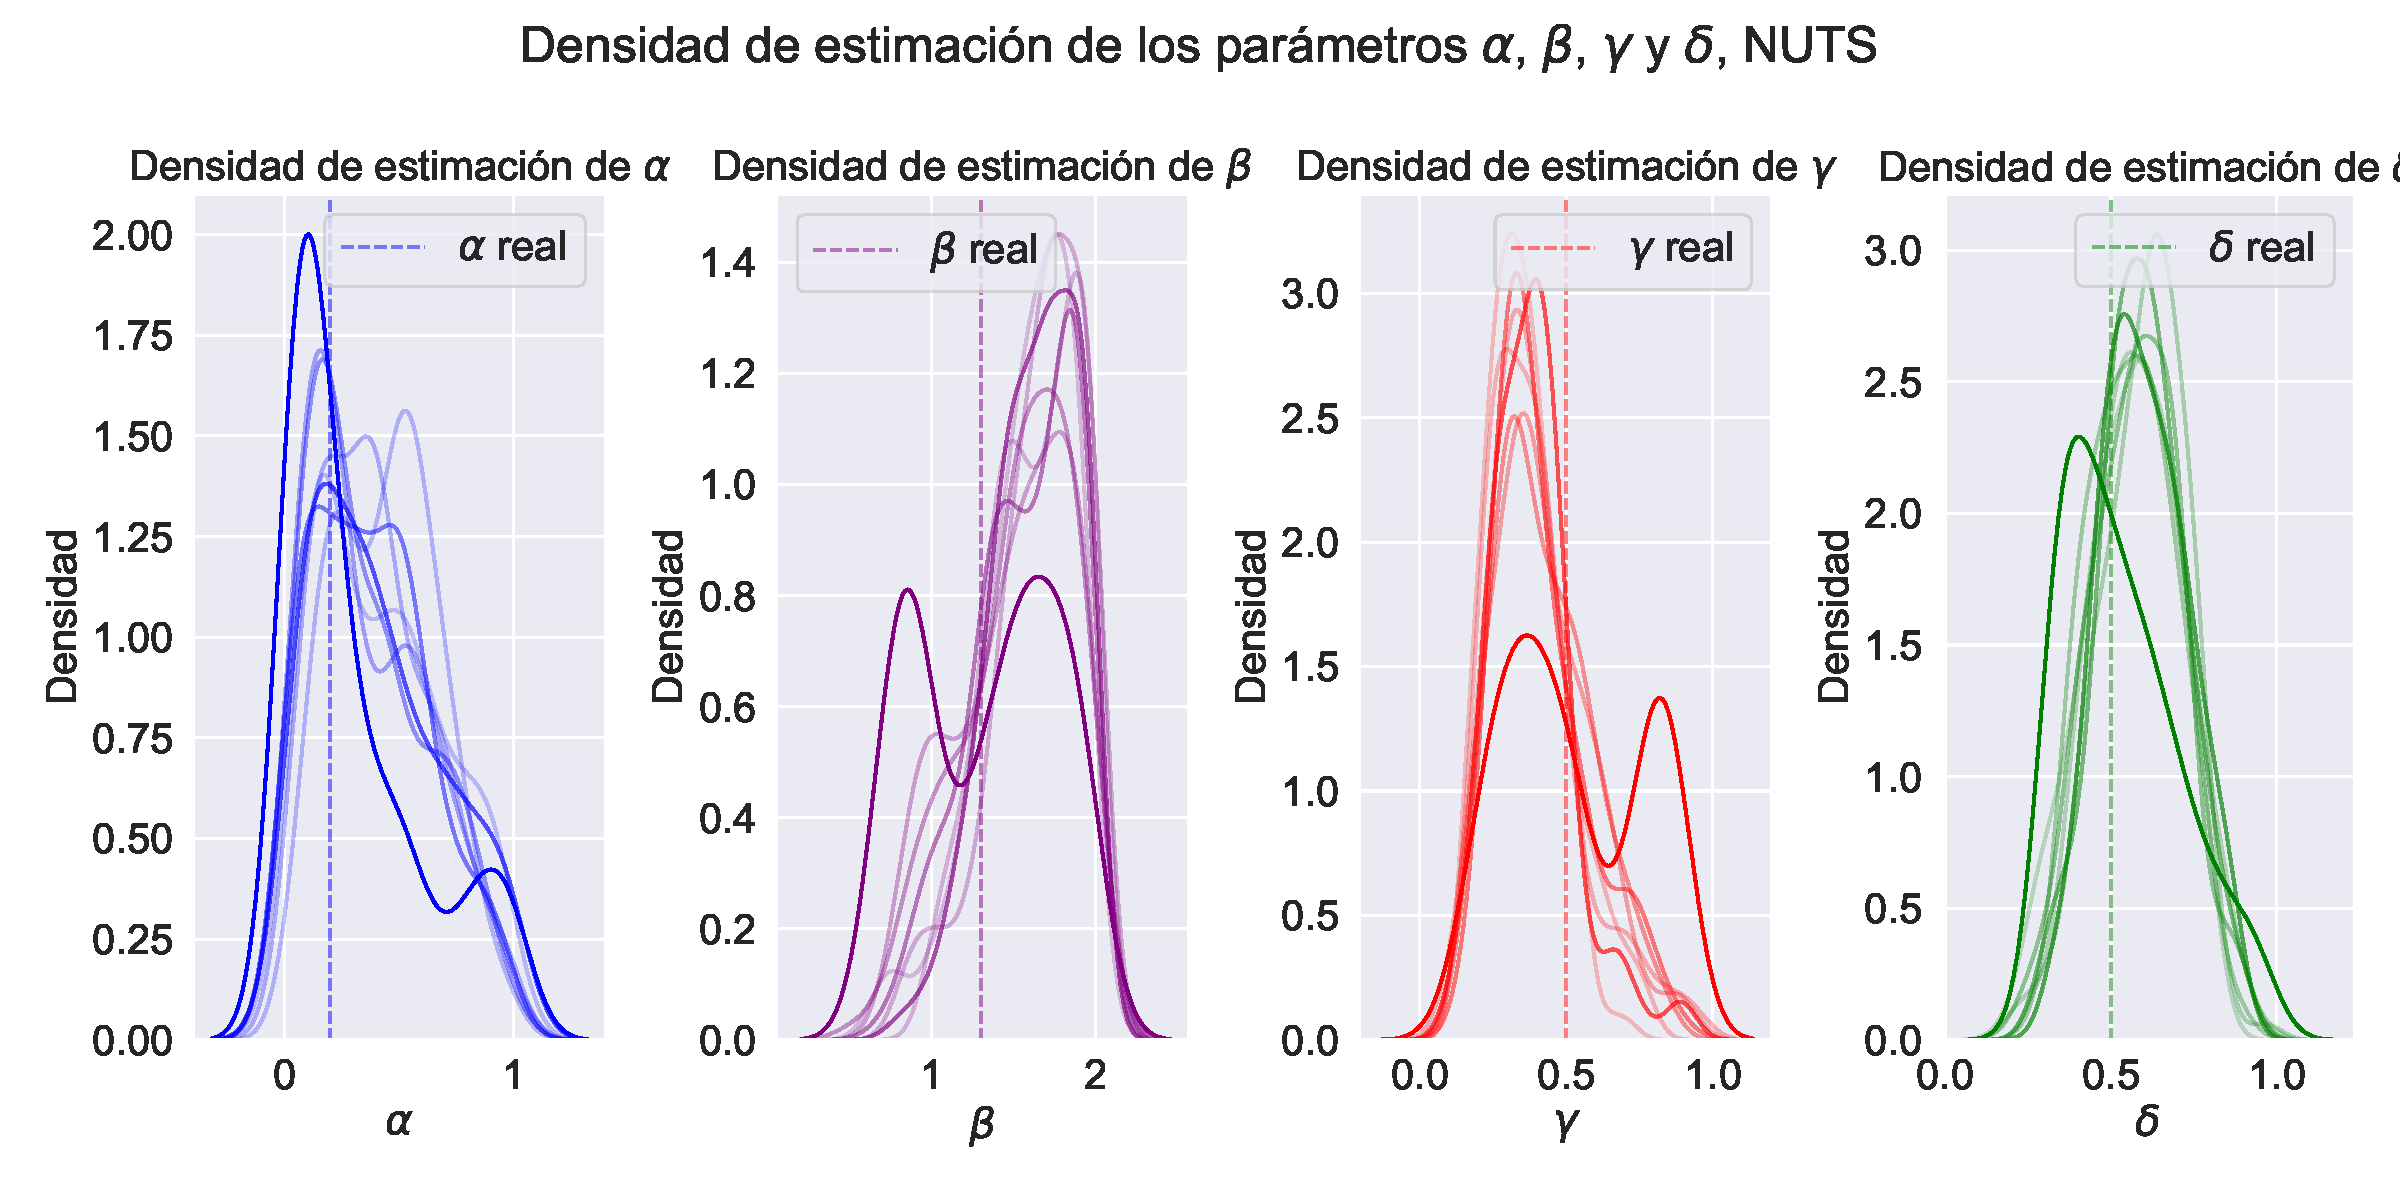
\includegraphics[width=0.55\linewidth]{img/content/chapter4/NUTS_seir_params_density.pdf}
        \caption{Densidad de las 8 cadenas.}
    \end{subfigure}
     \begin{subfigure}[b]{\linewidth}
        \centering
        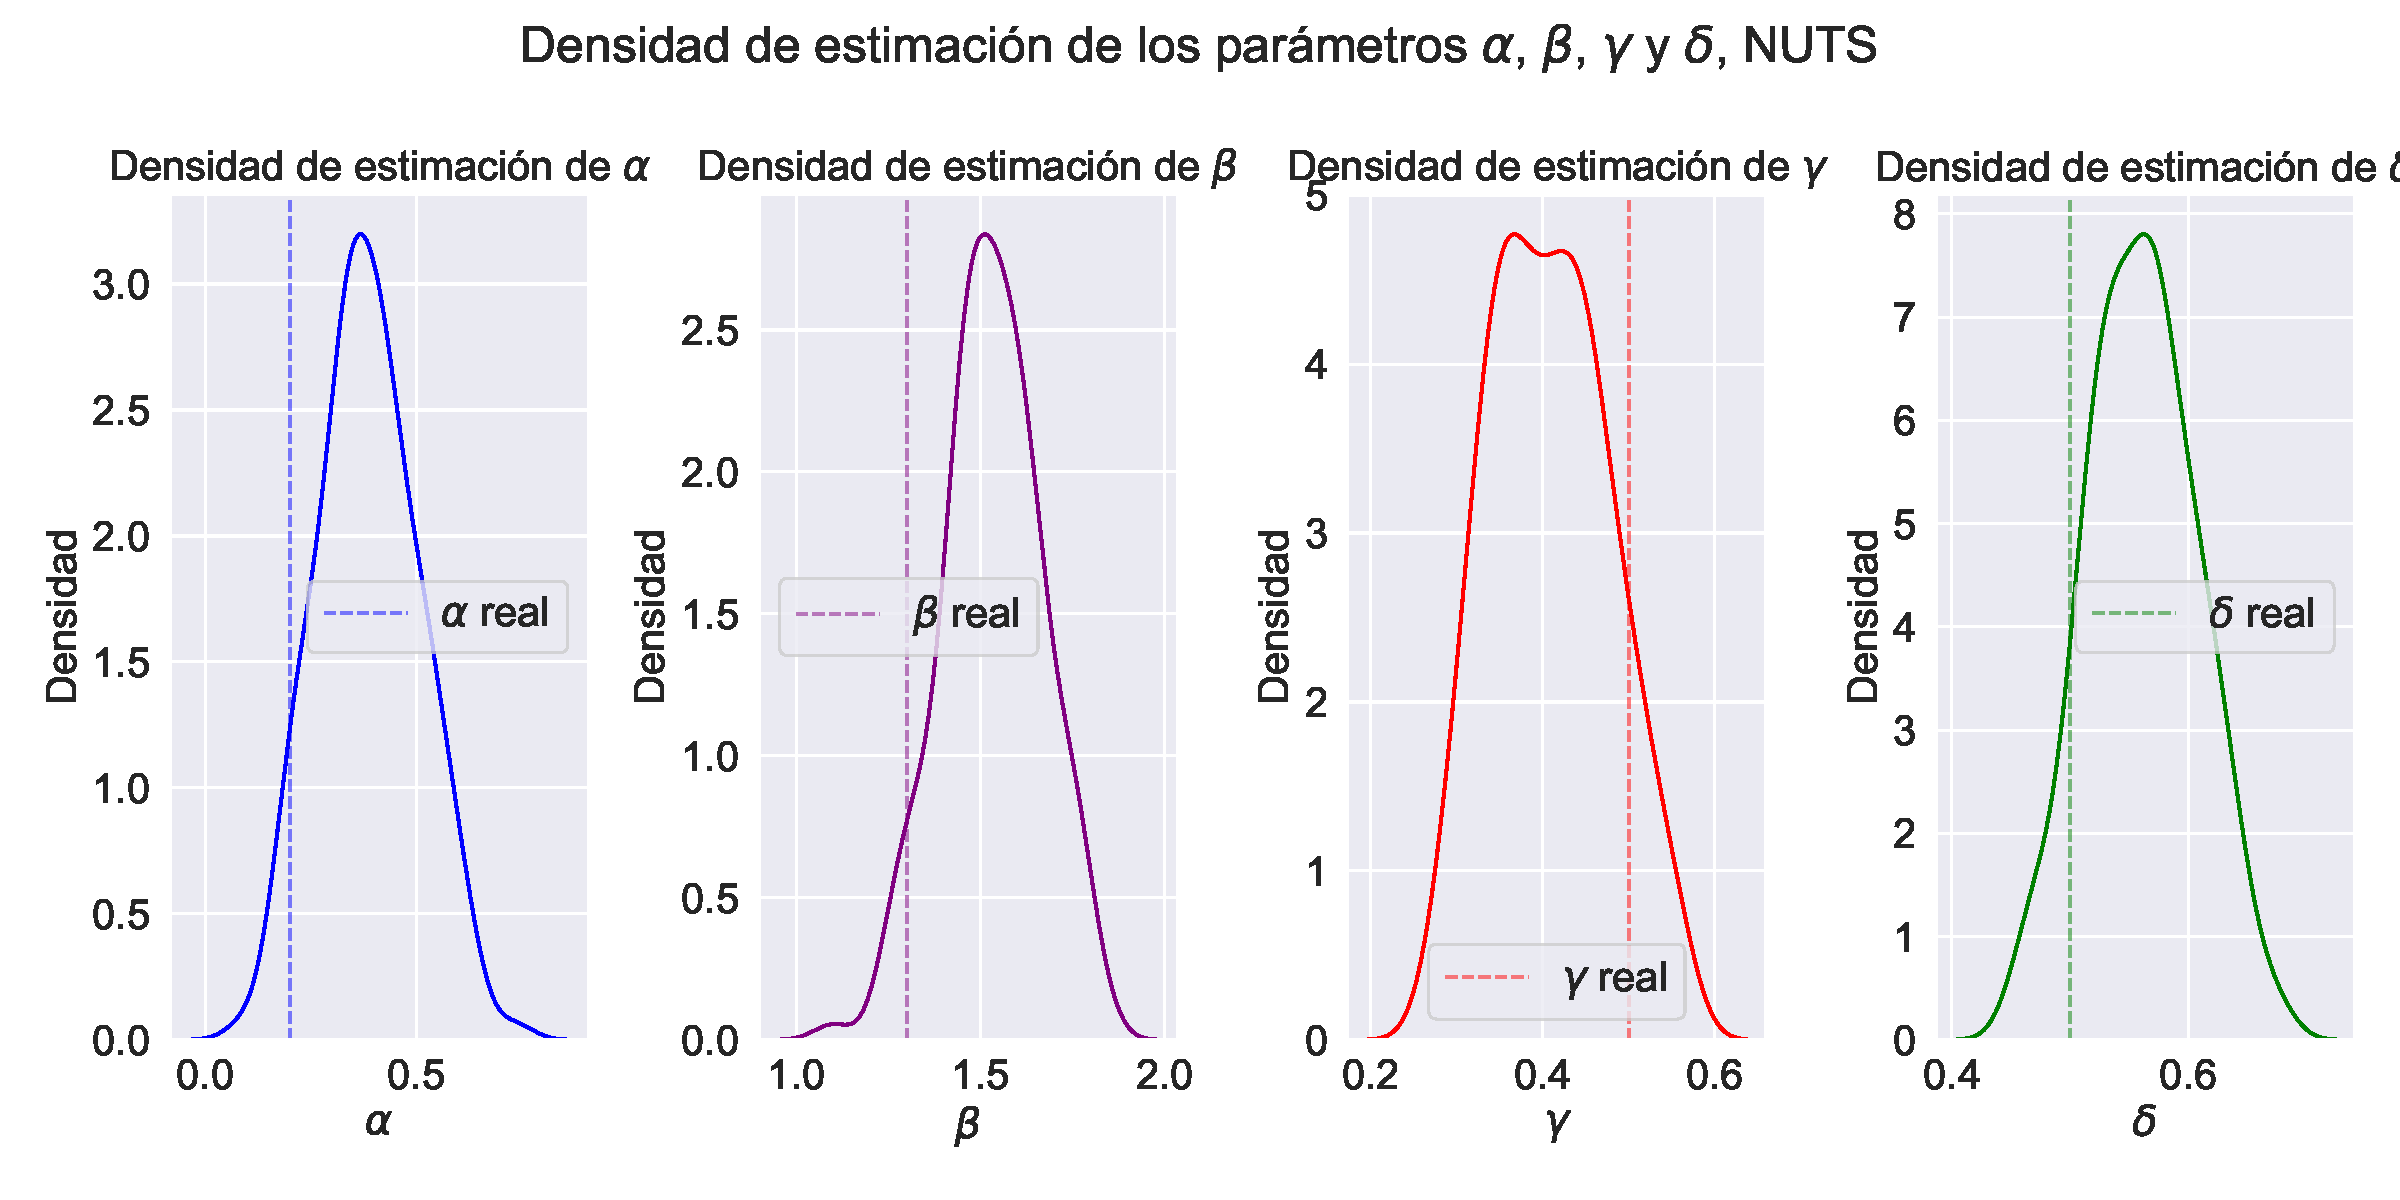
\includegraphics[width=0.55\linewidth]{img/content/chapter4/NUTS_seir_params_density_mean.pdf}
        \caption{Densidad promedio entre las 8 cadenas.}
    \end{subfigure}
    \caption{Densidad de los parámetros del modelo SEIR estimados con MCMC con \textit{sampler} NUTS.}
\end{figure}